
% !TEX program = xelatex

\documentclass[12pt]{article}

% ==================================================
% 1. PAGE LAYOUT
% ==================================================
\usepackage[
    letterpaper,
    margin=0.75in,
    headheight=14.5pt,
    headsep=0.22in,
    footskip=0.35in
]{geometry}

% ==================================================
% 2. FONT AND LANGUAGE
% ==================================================
\usepackage{fontspec}
\defaultfontfeatures{Ligatures=TeX}
\setmainfont{TeX Gyre Termes}

% ==================================================
% 3. REQUIRED PACKAGES
% ==================================================
\usepackage{amssymb}
\usepackage{array}
\usepackage{enumitem}
\usepackage{environ}
\usepackage{fancyhdr}
\usepackage{graphicx}
\usepackage{longtable}
\usepackage{needspace}
\usepackage{setspace}
\usepackage{tabularx}
\usepackage{titlesec}
\usepackage{xcolor}
\usepackage{hyperref}

% ==================================================
% 4. DOCUMENT COLORS AND FORMATTING
% ==================================================
\definecolor{HCMUSBlue}{RGB}{0,112,192}

\setlength{\parindent}{0pt}
\setlength{\parskip}{0pt}

\setstretch{1.5}

\setcounter{secnumdepth}{2}
\setcounter{tocdepth}{2}

% ==================================================
% 5. SECTION FORMATTING
% ==================================================
\titleformat{\section}
    {\color{HCMUSBlue}\bfseries\fontsize{22}{27}\selectfont}
    {\thesection}
    {0.5em}
    {}

\titleformat{\subsection}
    {\bfseries\fontsize{16}{20}\selectfont}
    {\thesubsection}
    {0.6em}
    {}

\titlespacing*{\section}
    {0pt}{12pt}{6pt}

\titlespacing*{\subsection}
    {0pt}{10pt}{4pt}

% ==================================================
% 6. TABLE AND DOCUMENT COMMANDS
% ==================================================
\newcolumntype{L}{>{\raggedright\arraybackslash}X}

\newcommand{\blankcell}{\rule{0pt}{2.6ex}}

\NewEnviron{srstable}[1]{%
    \begin{center}
        \small
        \renewcommand{\arraystretch}{1.2}
        \setlength{\tabcolsep}{4pt}
        \begin{tabularx}{\textwidth}{|#1|}
            \hline
            \BODY
        \end{tabularx}
    \end{center}
}

\newcommand{\templatehint}[1]{%
    \par\textit{#1}\par
}

\newcommand{\diagramplaceholder}[1]{%
    \begin{center}
        \fbox{%
            \parbox[c][1.25in][c]{0.88\textwidth}{%
                \centering\textit{#1}%
            }%
        }
    \end{center}
}

% ==================================================
% 7. TABLE OF CONTENTS
% ==================================================
\makeatletter

\renewcommand{\tableofcontents}{%
    \begin{center}
        {\color{HCMUSBlue}
        \bfseries
        \fontsize{30}{36}\selectfont
        Table of Contents\par}
    \end{center}

    \vspace{0.5\baselineskip}

    {\setstretch{1.0}\@starttoc{toc}}%
}

\makeatother

% ==================================================
% 8. HEADER AND FOOTER
% ==================================================
\pagestyle{fancy}

\fancyhf{}

\fancyhead[L]{\small Introduction to Software Engineering}
\fancyhead[R]{\small Room4U -- Software Design}

\fancyfoot[L]{\small HCMUS}
\fancyfoot[C]{\small SE Dept.}
\fancyfoot[R]{\small\thepage}

\renewcommand{\headrulewidth}{0pt}
\renewcommand{\footrulewidth}{0pt}

\setlength{\headheight}{14.5pt}

% ==================================================
% 9. DOCUMENT CONTENT
% ==================================================
% Reduce horizontal padding in tables
\setlength{\tabcolsep}{3pt}

% Improve automatic line breaking
\usepackage{microtype}
\setlength{\emergencystretch}{3em}


\begin{document}

\pagenumbering{roman}

% --------------------------------------------------
% 9.1. COVER PAGE
% --------------------------------------------------
\begin{titlepage}

    \thispagestyle{empty}

    \vspace*{0.35in}

    \begin{center}

        {\bfseries
        \fontsize{22}{28}\selectfont
        Introduction to Software Engineering\par}

        \vspace{1.15in}

        {\bfseries
        \fontsize{24}{30}\selectfont
        Software Design\par}

    \end{center}

    \vspace{0.65in}

    {\fontsize{14}{20}\selectfont
    The student team is required to complete the Software
    Design documentation for the assigned course project,
    following the attached template.\par}

    \vfill

    \begin{center}

        
\includegraphics[width=1.1in]{images/hcmus-logo.png}

        \par\vspace{0.25in}

        Software Engineering Department

        \par\vspace{0.1in}

        Faculty of Information and Technology

        \par\vspace{0.1in}

        University of Science

    \end{center}

\end{titlepage}

% --------------------------------------------------
% 9.2. TABLE OF CONTENTS
% --------------------------------------------------
\clearpage

\newgeometry{margin=1in}

\thispagestyle{empty}

\tableofcontents

\clearpage

\restoregeometry

% --------------------------------------------------
% 9.3. MAIN DOCUMENT
% --------------------------------------------------
\pagenumbering{arabic}

\pagestyle{fancy}

\begin{center}
    {\color{HCMUSBlue}
    \bfseries
    \fontsize{40}{48}\selectfont
    Software Design\par}
\end{center}

% ==================================================
% 10. PROJECT SECTIONS
% ==================================================

\section{Objectives}
Specify how the Room4U system will realize the accepted PA2 Software Requirements Specification behavior without expanding the five committed feature groups. This proposal translates functional and non-functional requirements into concrete architectural, object-oriented, data, and interface specifications, making access permissions, current-state validation, concurrency controls, audit and history retention, and error outcomes actionable for implementation and PA4 test design.

In accordance with the supplied PA3 template, this document establishes:
\begin{itemize}[leftmargin=1.5em,itemsep=2pt,topsep=2pt]
  \item \textbf{System Architecture:} C4 context, container, component, and deployment views alongside formal Architecture Decision Records (ADRs).
  \item \textbf{Object-Oriented Design:} A conceptual domain model, design class diagrams, eight core class specifications, five main-flow sequence diagrams with alternative and exception paths, and state machine models.
  \item \textbf{Data and Interface Design:} Relational data specifications (ERD, constraints, and indexing) and UI/UX wireframes and control specifications.
  \item \textbf{Verification and Traceability:} Bidirectional traceability linking all 55 PA2 requirement and business rule entries to proposed PA3 design artifacts.
\end{itemize}

\clearpage

\section{Member Contribution Assessment}


\begin{srstable}{p{0.13\textwidth}|p{0.18\textwidth}|p{0.22\textwidth}|p{0.16\textwidth}|L}
\textbf{ID} & \textbf{Name} & \textbf{Planned Role(s)} & \shortstack{\textbf{Actual Share}\\\textbf{(\%)}} & \textbf{Evidence} \\ \hline

22127245 & Nguyễn Thành Long & PM / traceability and review & 25\% & \href{https://github.com/T03-R4U/ROOM4U/issues/44}{GitHub Issue \#44} \\ \hline

24127127 & Lại Minh Thông & Domain / UML / testability & 25\% & \href{https://github.com/T03-R4U/ROOM4U/issues/42}{GitHub Issue \#42} \\ \hline

24127461 & Nguyễn Kim Ngân & UI / document assembly & 25\% & \href{https://github.com/T03-R4U/ROOM4U/issues/43}{GitHub Issue \#43} \\ \hline

24127506 & Trần Thiên Phúc & Architecture / database & 25\% & \href{https://github.com/T03-R4U/ROOM4U/issues/40}{GitHub Issue \#40}, \href{https://github.com/T03-R4U/ROOM4U/issues/41}{GitHub Issue \#41}\\ \hline

\end{srstable}

\clearpage


% ==================================================
% SECTION 3 — DESIGN OVERVIEW
% ==================================================

\section{Design Overview}

Room4U is an independent web-based simulation for one university library. Student and Administrator accounts are created in advance. Students submit booking requests with Pending status, and Administrators manually approve or reject them. Pending requests do not reserve a room. Approved bookings and active maintenance blocks make their intervals unavailable. Adjacent intervals that only meet at an endpoint do not overlap. The system does not integrate with the real library or university SSO [P1, P2].

The design uses a browser-based web client, a Node.js/Express backend API and a PostgreSQL database. Firebase Authentication provides identity verification, while the Room4U backend enforces application roles, request ownership and booking rules. Architectural responsibilities and deployment are detailed in Section 4, object-oriented models in Section 5, data structures in Section 6 and user interactions in Section 7.

\subsection{Design Goals and Constraints}

The following requirements have a significant influence on the design. The design responses describe how the system is intended to satisfy them; they do not represent measured implementation results.

\begin{longtable}{|p{0.19\textwidth}|p{0.43\textwidth}|p{0.30\textwidth}|}
\hline
\textbf{Requirement driver} & \textbf{Design goal and response} & \textbf{Acceptance basis} \\
\hline
\endfirsthead
\hline
\textbf{Requirement driver} & \textbf{Design goal and response} & \textbf{Acceptance basis} \\
\hline
\endhead
FR-15--16; BR-08; NFR-03 &
Coordinate concurrent room updates and revalidate current request, room and schedule data before committing an approval. &
Conflicting approvals must not both succeed, and an Approved booking must not overlap active maintenance. \\
\hline
FR-21; BR-14 &
Coordinate capacity changes with booking approvals and check current future Approved bookings when saving room details. &
A future Approved booking must never have a group size greater than the room's saved capacity. \\
\hline
FR-02--04; NFR-02 &
Enforce identity, role and ownership checks in the backend, and return only data the caller is permitted to view. &
Invalid identity receives 401; role or ownership violations receive 403 without protected data disclosure. \\
\hline
FR-19; NFR-10 &
Retain ordered booking-request creation and status-transition events with identifiable actors and timestamps. &
Earlier events remain retrievable and are not overwritten by later actions. \\
\hline
NFR-09 &
Commit related status, occupancy and history changes together, and preserve the prior state when validation or persistence fails. &
Failed operations leave no partial state change or orphan history event. \\
\hline
NFR-01 &
Support efficient room-search and own-request queries through suitable indexes, bounded responses and controlled database access. &
P95 server response time is at most two seconds under the reference workload defined in PA2 Section 6.2. \\
\hline
NFR-04--05; NFR-07; NFR-11--12 &
Provide Vietnamese, responsive interfaces with keyboard access, visible focus, labelled controls, understandable statuses and corrective error messages. &
Accessibility, usability, browser compatibility and localization are verified against the conditions in PA2 Section 6.2. \\
\hline
NFR-06 &
Use HTTPS and restrict the handling of credentials, identity tokens and application-controlled logs. &
Source, repository history and application-controlled logs contain no prohibited secrets or full identity tokens; deployed application traffic uses HTTPS. \\
\hline
NFR-08 &
Define a verified pre-demo backup and a documented database restoration procedure. &
Restoration on the reference environment completes within 30 minutes and preserves records committed before the backup point. \\
\hline
\end{longtable}

The initial demonstration dataset contains eight simulated rooms, two Student accounts and one Administrator account. The system supports up to 500 pre-created accounts. Since room creation is supported, eight rooms represent the initial dataset rather than a permanent maximum [P2].

The reference environment is a Linux server with 2 vCPUs, 4 GB RAM and 20 GB storage, hosting one backend instance and one database. Node.js/Express, PostgreSQL and Firebase Authentication follow the technology baseline described in PA1 and PA2. Environment configuration and feasibility must be checked before deployment, and quality targets remain subject to verification [P1, P2].

The design must remain feasible for a four-member student team within the PA1 schedule. PA3 design work is planned for course Weeks 6--7; the official submission date and time follow Moodle announcements. These constraints favour a small deployment and clearly separated responsibilities that support parallel development and review [P1].

PA1 assumes free or student-tier development tools and a provisional hosting allowance of VND 500,000 for the course demonstration. Infrastructure choices must be assessed against this allowance and the reference environment. Changes affecting scope, cost or schedule follow the project change-control process [P1].

\subsection{Accepted PA2 Decisions and Design Implications}

The accepted PA2 Software Requirements Specification is the requirements baseline for this design. Decisions D01--D08 provide the booking policies and quality targets used throughout PA3 [P2].

\begin{longtable}{|p{0.14\textwidth}|p{0.43\textwidth}|p{0.35\textwidth}|}
\hline
\textbf{PA2 decision} & \textbf{Baseline used in PA3} & \textbf{Design implications} \\
\hline
\endfirsthead
\hline
\textbf{PA2 decision} & \textbf{Baseline used in PA3} & \textbf{Design implications} \\
\hline
\endhead
D01--D02 &
Bookings fall within 08:00--20:00 on one local date. At submission and approval, now $<$ start $\leq$ now + 7 days. Start and end times use :00 or :30 marks, with durations of 30, 60, 90 or 120 minutes. &
Centralized time validation uses the server's current decision time and Asia/Ho\_Chi\_Minh. Forms use duration input, and the backend derives the end time. \\
\hline
D03 &
The measurable quality targets and verification conditions are defined in PA2 Section 6.2. &
Architecture, queries, interfaces and operational procedures are designed to support these targets. Compliance requires subsequent measurement and evaluation. \\
\hline
D04 &
Required rejection, administrator-cancellation and maintenance reasons contain 1--250 characters after trimming. Room capacity is an integer from 1 to 50. &
Backend validation and appropriate database constraints enforce the limits. UI controls provide corresponding validation and corrective feedback. \\
\hline
D05 &
Suspension blocks new submissions and approvals while preserving existing bookings. Capacity changes must remain consistent with future Approved bookings, including during concurrent approval. &
Room-state changes, capacity edits and booking decisions use a coordinated update mechanism. Existing bookings are retained. \\
\hline
D06 &
A maintenance block may be removed only while active and before its start, after confirmation. Its record is retained. &
Maintenance has separate active and removed states. Removal releases only the block's occupancy effect and leaves booking records unchanged. \\
\hline
D07 &
Student and Administrator cancellations require server now $<$ booking start. Past-start Pending requests remain visible but cannot be approved or Student-cancelled; Administrators may reject them. &
Services check current status and server decision time before committing. The design introduces no automatic Expired status or expiry job. \\
\hline
D08 &
Room IDs remain stable. Shared calendars do not expose other students' booking identities. Booking status history and processing reasons are retained. &
Stable identifiers preserve references. Authorized DTOs restrict disclosure, and booking events are appended within the same transaction as request changes. \\
\hline
\end{longtable}

% !TEX root = ../main.tex

% Section 4 — Architectural Design

\section{Architectural Design}

\subsection{Architectural style}

Room4U uses a client–server architecture with a layered modular monolith (ADR-001). The browser provides the user interface, while a single application API controls access to business operations and a PostgreSQL database stores the application data.\par

Within the API, HTTP controllers handle routing, input DTOs and response translation. Access-control components establish the authenticated actor and application role. Application services coordinate use cases, domain objects and policies enforce business rules, and persistence components execute database operations. Domain rules do not depend on browser controls, Express request objects or SQL statements.\par

This structure supports the main design goals. Centralized role and ownership checks support NFR-02. A shared transactional boundary supports conflict prevention in FR-16 and consistent rollback in NFR-09. Separating HTTP handling, business rules and persistence allows these areas to be reviewed and changed with less impact on one another. The deployment remains manageable for the four-member team and the PA1 schedule.\par

The main trade-offs are additional interfaces between layers and a shared deployment lifecycle for the API modules. The initial deployment also provides no automatic failover. Performance and recovery must therefore be evaluated against the PA2 targets; the architectural choice alone does not demonstrate that those targets have been met.\par

\subsection{System context diagram}

\begin{center}

\begin{minipage}{0.96\textwidth}

\centering

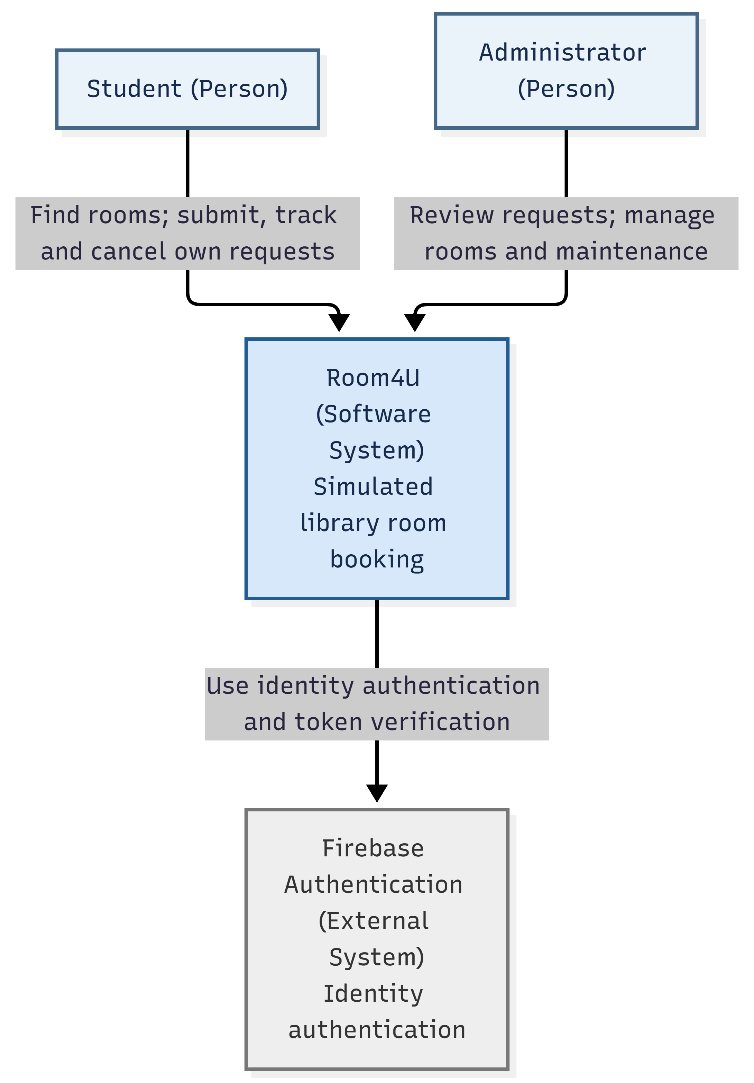
\includegraphics[width=\textwidth,height=0.62\textheight,keepaspectratio]{images/04-architectural-design-assets/architecture-figure-4.png}

\par\vspace{0.45em}

\emph{\textbf{Figure 4.2.} A01 C4 level 1. Room4U is the system boundary; its database is internal. Firebase supports identity only.}\par

\end{minipage}

\end{center}

\vspace{0.6em}



Students find rooms and manage only their own requests. Administrators process requests and manage rooms/maintenance. Instructors and the TA evaluate the coursework; they are not booking actors. Room4U does not contact the real university booking system.\par

\subsection{Container diagram}

\begin{center}

\begin{minipage}{0.96\textwidth}

\centering

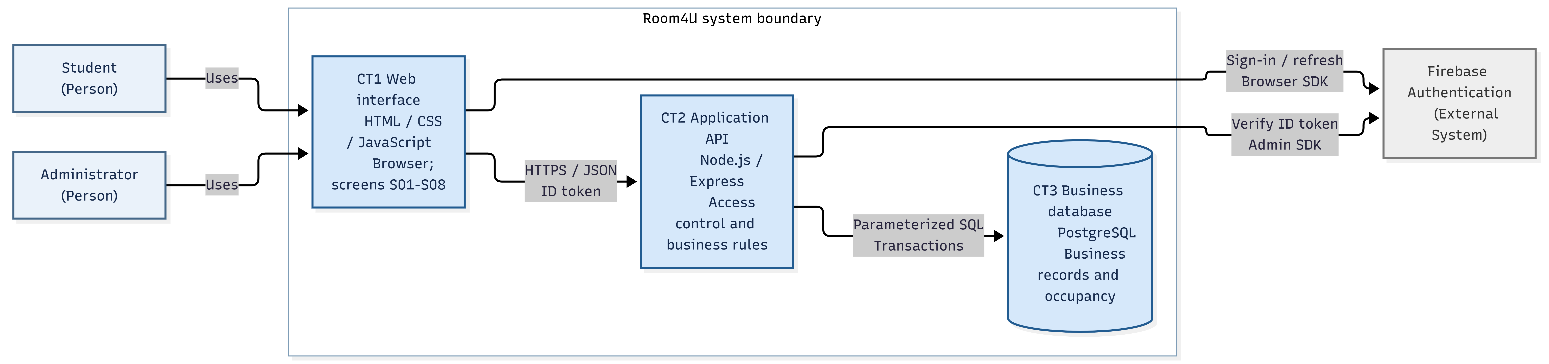
\includegraphics[width=\textwidth,height=0.62\textheight,keepaspectratio]{images/04-architectural-design-assets/architecture-figure-3.png}

\par\vspace{0.45em}

\emph{\textbf{Figure 4.3.} A02 C4 level 2. CT1 is browser JavaScript, CT2 the application API and CT3 the business database.}\par

\end{minipage}

\end{center}

\vspace{0.6em}



\begin{longtable}{|p{0.190\textwidth}|p{0.350\textwidth}|p{0.350\textwidth}|}

\hline

\textbf{Container} & \textbf{Responsibility} & \textbf{Technology and boundary} \\ \hline

\endfirsthead

\hline

\textbf{Container} & \textbf{Responsibility} & \textbf{Technology and boundary} \\ \hline

\endhead

CT1 Web interface & Render S01–S08; assist input; send authenticated commands.\allowbreak{} & HTML/\allowbreak{}CSS/\allowbreak{}Java\allowbreak{}Script; Firebase browser SDK; no authoritative rule decision.\allowbreak{} \\ \hline

CT2 Application API & Enforce roles/\allowbreak{}ownership/\allowbreak{}rules, transactions and safe DTOs.\allowbreak{} & Node.\allowbreak{}js/\allowbreak{}Express; Firebase Admin SDK; parameterized SQL through a pool.\allowbreak{} \\ \hline

CT3 Database & Persist business records and shared occupancy constraint.\allowbreak{} & Postgre\allowbreak{}SQL with btree\_\allowbreak{}gist; available only to the API/\allowbreak{}migration operator.\allowbreak{} \\ \hline

\end{longtable}

\vspace{2mm}

\subsection{Component decomposition}

\begin{center}

\begin{minipage}{0.96\textwidth}

\centering

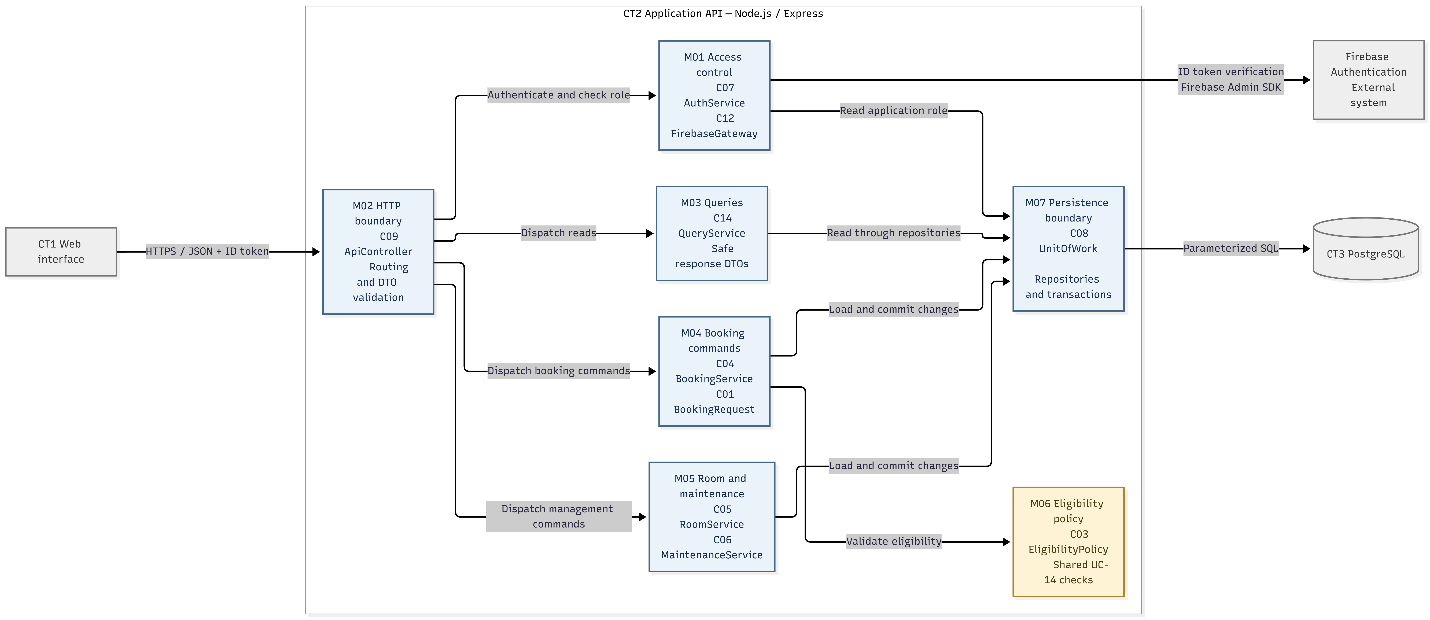
\includegraphics[width=\textwidth,height=0.62\textheight,keepaspectratio]{images/04-architectural-design-assets/architecture-figure-2.png}

\par\vspace{0.45em}

\emph{\textbf{Figure 4.4.} A03 Components inside CT2. M02 invokes access control before dispatching queries or commands.}\par

\end{minipage}

\end{center}

\vspace{0.6em}



\begin{longtable}{|p{0.190\textwidth}|p{0.350\textwidth}|p{0.350\textwidth}|}

\hline

\textbf{ID} & \textbf{Component responsibility} & \textbf{Related classes} \\ \hline

\endfirsthead

\hline

\textbf{ID} & \textbf{Component responsibility} & \textbf{Related classes} \\ \hline

\endhead

M01 & Verify identity and role; deny unauthorized access.\allowbreak{} & C07 Auth\allowbreak{}Service; C12 Firebase\allowbreak{}Gateway \\ \hline

M02 & HTTP routing, DTO validation and domain-\allowbreak{}error translation.\allowbreak{} & C09 Api\allowbreak{}Controller \\ \hline

M03 & Search, safe calendar DTO, owned history and admin queue.\allowbreak{} & C14 Query\allowbreak{}Service; read repositories \\ \hline

M04 & Submit/\allowbreak{}approve/\allowbreak{}reject/\allowbreak{}cancel with history.\allowbreak{} & C04 Booking\allowbreak{}Service; C01 Booking\allowbreak{}Request \\ \hline

M05 & Room details/\allowbreak{}state and maintenance commands.\allowbreak{} & C05 Room\allowbreak{}Service; C06 Maintenance\allowbreak{}Service; C02; C10 \\ \hline

M06 & Common UC-\allowbreak{}14 eligibility checks without writes.\allowbreak{} & C03 Eligibility\allowbreak{}Policy \\ \hline

M07 & One-\allowbreak{}client transaction, room guard, repositories and projections.\allowbreak{} & C08 Unit\allowbreak{}Of\allowbreak{}Work \\ \hline

\end{longtable}

\vspace{2mm}

M02 invokes M01 to establish the authenticated actor and check the required application role before dispatching a protected operation. Resource-specific ownership checks are performed after the requested record is loaded and before its data is returned or changed.\par

Read operations are dispatched to M03, which uses read repositories and returns explicitly selected DTO fields. Booking commands are dispatched to M04; room and maintenance commands are dispatched to M05. M04 invokes M06 for the shared UC-14 eligibility checks used by submission and approval. Command services use M07 to load current decision data and commit the complete set of changes within one transaction.\par

The component diagram shows dependencies between modules. The transaction order for state-changing operations is defined in Section 4.6.\par

\subsection{Deployment design}

\begin{center}

\begin{minipage}{0.96\textwidth}

\centering

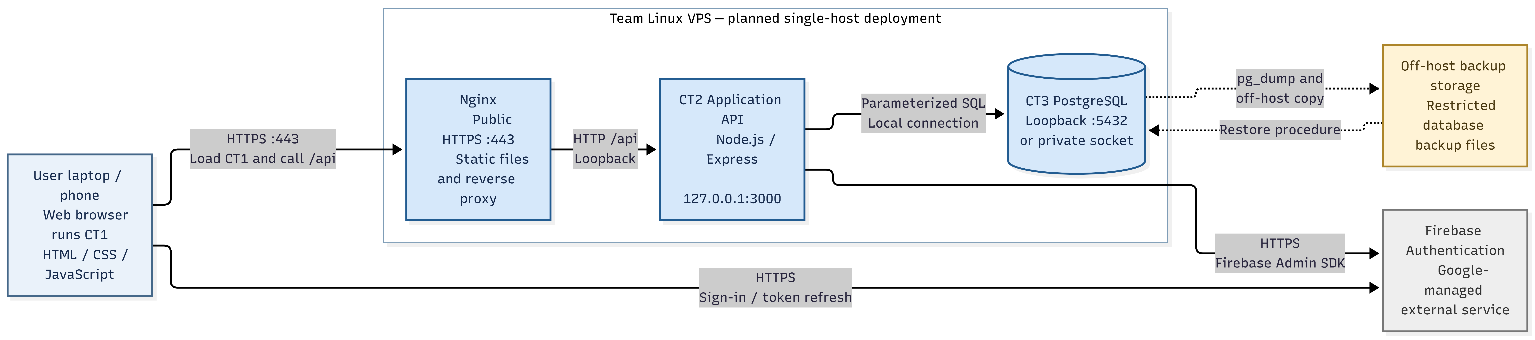
\includegraphics[width=\textwidth,height=0.62\textheight,keepaspectratio]{images/04-architectural-design-assets/architecture-figure-1.png}

\par\vspace{0.45em}

\emph{\textbf{Figure 4.5.} A04 Proposed deployment. Public access terminates at Nginx; API and database listen on private interfaces.}\par

\end{minipage}

\end{center}

\vspace{0.6em}



Nginx serves static assets and reverse-proxies /api to Express over loopback. PostgreSQL is not publicly exposed. Use one same-origin HTTPS site, explicit environment configuration and a restricted service account. Firebase credentials remain outside Git. The frontend uses Firebase-managed session state rather than copying full tokens into custom persistent storage.\par

Before PA5 demonstration: provision a clean database, apply reviewed migrations, seed test identities/roles and eight rooms, verify token handling, start the API behind Nginx and inspect a smoke path. Take a restricted database backup, copy it off-host and record the backup point. The restore drill must compare room/request/event IDs and counts and meet the PA2 recovery target. These are planned operations, not recorded successes.\par

The initial deployment places Nginx, the API and PostgreSQL on one VPS. This reduces deployment and administration work, but the host is a shared point of failure and its resources are shared by the application and database. Off-host backups support recovery; they do not provide automatic failover. The recovery procedure will be evaluated against NFR-08.\par

\subsection{Transaction protocol and schedule invariants}

\begin{longtable}{|p{0.190\textwidth}|p{0.350\textwidth}|p{0.350\textwidth}|}

\hline

\textbf{ID} & \textbf{Invariant} & \textbf{Enforcement} \\ \hline

\endfirsthead

\hline

\textbf{ID} & \textbf{Invariant} & \textbf{Enforcement} \\ \hline

\endhead

I01 & A Pending/\allowbreak{}Rejected/\allowbreak{}Cancelled request has no occupancy projection.\allowbreak{} & C04 status Change\allowbreak{}Set; C08 same-\allowbreak{}client transaction.\allowbreak{} \\ \hline

I02 & An Approved request has exactly one occupancy row matching its room and interval.\allowbreak{} & Unique booking source; composite FK; central command protocol.\allowbreak{} \\ \hline

I03 & An active maintenance block has one matching occupancy row; a removed block has none.\allowbreak{} & Unique maintenance source; composite FK; C06 create/\allowbreak{}remove transaction.\allowbreak{} \\ \hline

I04 & No two room\_\allowbreak{}occupancy intervals overlap for the same room.\allowbreak{} & Gi\allowbreak{}ST exclusion on room\_\allowbreak{}id and half-\allowbreak{}open tstzrange.\allowbreak{} \\ \hline

I05 & A capacity edit preserves all future Approved group sizes.\allowbreak{} & Same persistent room guard for capacity save and approval; current reread.\allowbreak{} \\ \hline

I06 & Every successful booking creation/\allowbreak{}transition adds one event; refused commands add none.\allowbreak{} & Request/\allowbreak{}status/\allowbreak{}occupancy/\allowbreak{}event commit or rollback together.\allowbreak{} \\ \hline

I07 & Suspension blocks subsequent submission/\allowbreak{}approval, not existing occupancy.\allowbreak{} & Room state rechecked inside the guard; retain source/\allowbreak{}projection rows.\allowbreak{} \\ \hline

I08 & Public calendar data contains availability without another student identity.\allowbreak{} & M03 explicit DTO allowlist; detail routes enforce owner/\allowbreak{}Admin.\allowbreak{} \\ \hline

\end{longtable}

\vspace{2mm}

All commands affecting an existing room use this order: authorize the actor; obtain the target room ID without exposing protected data; BEGIN at READ COMMITTED; SELECT the persistent rooms row FOR UPDATE; load the current target and occupancy; capture server decision time; validate; save the complete ChangeSet; COMMIT; then return success. If any step fails, ROLLBACK and release the same pool client. Creating a new room is the only command without an existing room guard; normalized code uniqueness is enforced by PostgreSQL.\par

Use a fresh UnitOfWork for each command. Never share a checked-out client between concurrent requests, and never perform Firebase calls while holding the room lock. All booking/maintenance/state/capacity writers must follow this protocol, including future API instances. If a command ever spans several rooms, acquire room IDs in sorted order; no such operation is currently exposed.\par

Locking only overlapping booking rows is insufficient when no matching row exists. The room row is a stable guard even for an empty schedule. PostgreSQL row locks hold until transaction end [R1]. The database exclusion constraint adds protection across both booking and maintenance projections [R2]. I01–I03 and event correspondence also depend on the centralized transaction writer; the exclusion constraint alone does not prove them.\par

After waiting for the room lock, validation queries run as subsequent READ COMMITTED statements and therefore see committed preceding room writes [R5]. The injected decision clock is sampled after that wait, not from a transaction-start timestamp. In PostgreSQL use a fresh clock\_timestamp() result (or equivalent server clock) for the decision; reject non-finite timestamps and start values with nonzero seconds/subseconds. Local-hour and same-date checks use Asia/Ho\_Chi\_Minh.\par

Lock order is room row first, then the target request/block if a separate record lock is needed. A database lock timeout is an operational failure, not proof that the room is booked. An unknown commit outcome is reconciled by reading the resource or replaying the original submission key; the client must not create a new key automatically.\par

\subsubsection{Race outcomes to preserve}

\begin{longtable}{|p{0.190\textwidth}|p{0.350\textwidth}|p{0.350\textwidth}|}

\hline

\textbf{Concurrent actions} & \textbf{Permitted outcome} & \textbf{Refusal behavior} \\ \hline

\endfirsthead

\hline

\textbf{Concurrent actions} & \textbf{Permitted outcome} & \textbf{Refusal behavior} \\ \hline

\endhead

Two overlapping approvals & One commits; the second rechecks and finds occupancy.\allowbreak{} & Second stays Pending; no new event.\allowbreak{} \\ \hline

Approval vs maintenance creation & The first valid command occupies the interval.\allowbreak{} & Second refuses overlap; never both occupied.\allowbreak{} \\ \hline

Approval vs suspension & Approval first: booking retained.\allowbreak{} Suspension first: new approval denied.\allowbreak{} & No automatic cancellation.\allowbreak{} \\ \hline

Approval vs capacity reduction & Approval first: capacity save checks its group.\allowbreak{} Edit first: approval uses new capacity.\allowbreak{} & Unsafe action refused; invariant I05 holds.\allowbreak{} \\ \hline

Owner cancel vs approval & Room guard orders decisions.\allowbreak{} Cancelled cannot later be approved.\allowbreak{} & If state changed, report current outcome; no duplicate event.\allowbreak{} \\ \hline

Removal vs passage of start time & Removal checks active state and decision time after the guard.\allowbreak{} & At/\allowbreak{}after start, refuse removal and retain occupancy.\allowbreak{} \\ \hline

Repeated command /\allowbreak{} lost response & A creation replay reuses owner/\allowbreak{}submission\allowbreak{}Key; decisions reread state.\allowbreak{} & Never infer success from a timeout; refresh authoritative state.\allowbreak{} \\ \hline

\end{longtable}

\vspace{2mm}

C08 implements this shared transaction boundary for every room command. The schema example and full proposed SQL source are described in Section 6. Validation, authorization and rollback paths remain part of each service operation.\par

\subsection{Architecture Decision Records}

The following ADRs document the proposed architectural decisions, their context, alternatives and consequences. Their current status is Accepted. Each ADR is to be maintained as a separate record under docs/design/adr/, consistent with the PA3 template.\par

\subsubsection{ADR-001 Use a layered modular monolith}

\begin{longtable}{|p{0.200\textwidth}|p{0.740\textwidth}|}

\hline

\textbf{Field} & \textbf{Record} \\ \hline

\endfirsthead

\hline

\textbf{Field} & \textbf{Record} \\ \hline

\endhead

Status & Accepted \\ \hline

Context & Four students must implement five feature groups within the PA1 schedule.\allowbreak{} Booking and availability changes need one reliable transactional boundary.\allowbreak{} \\ \hline

Decision & Use a browser client and one Express deployment.\allowbreak{} Separate HTTP/\allowbreak{}access control, queries, command services, domain policies and persistence.\allowbreak{} Keep the application tables in one Postgre\allowbreak{}SQL database; ADR-\allowbreak{}005 refines the model to seven tables.\allowbreak{} \\ \hline

Alternatives considered & Microservices: adds distributed authorization, deployment and consistency work.\allowbreak{} A single unstructured Express file: initially shorter but mixes rules, HTTP and SQL.\allowbreak{} \\ \hline

Consequences & The design provides a small deployment and a local transaction boundary for booking decisions.\allowbreak{} Separating responsibilities allows services and policies to be verified through injected dependencies.\allowbreak{} Module boundaries must be maintained during implementation and code review.\allowbreak{} API modules are deployed together, and the initial single-\allowbreak{}instance deployment provides no automatic failover.\allowbreak{} Application and database resource usage must be evaluated on the PA1 reference environment before claiming compliance with the PA2 performance targets.\allowbreak{} \\ \hline

\end{longtable}

\vspace{2mm}

\subsubsection{ADR-002 Serialize room writes and share one occupancy constraint}

\begin{longtable}{|p{0.200\textwidth}|p{0.740\textwidth}|}

\hline

\textbf{Field} & \textbf{Record} \\ \hline

\endfirsthead

\hline

\textbf{Field} & \textbf{Record} \\ \hline

\endhead

Status & Accepted \\ \hline

Context & Two approvals, maintenance creation, suspension and capacity edits must make consistent decisions even when the room initially has no occupied interval.\allowbreak{} \\ \hline

Decision & At READ COMMITTED, lock the persistent rooms row before loading current decision data.\allowbreak{} Use the same lock for every command affecting that room.\allowbreak{} Represent Approved bookings and active maintenance in room\_\allowbreak{}occupancy, protected by a room/\allowbreak{}range Gi\allowbreak{}ST exclusion constraint.\allowbreak{} \\ \hline

Alternatives considered & Check then write without a lock: both requests can pass.\allowbreak{} Lock only overlapping booking rows: locks no guard when the set is empty.\allowbreak{} An in-\allowbreak{}memory mutex: does not protect another API process.\allowbreak{} SERIALIZABLE with retries: viable, but more retry handling than the selected explicit room guard.\allowbreak{} \\ \hline

Consequences & Different rooms can progress concurrently; writes for one room wait for each other.\allowbreak{} The occupancy projection adds transactional maintenance work and btree\_\allowbreak{}gist must be available.\allowbreak{} Centralized write paths, source foreign keys and rollback checks are required.\allowbreak{} Validate the migration and races in PA5.\allowbreak{} \\ \hline

\end{longtable}

\vspace{2mm}

\subsubsection{ADR-003 Use Firebase identity with application role checks}

\begin{longtable}{|p{0.200\textwidth}|p{0.740\textwidth}|}

\hline

\textbf{Field} & \textbf{Record} \\ \hline

\endfirsthead

\hline

\textbf{Field} & \textbf{Record} \\ \hline

\endhead

Status & Accepted \\ \hline

Context & PA1 uses Firebase Authentication and pre-\allowbreak{}created accounts.\allowbreak{} Room4U still owns Student/\allowbreak{}Admin permissions and request ownership; there is no university SSO integration.\allowbreak{} \\ \hline

Decision & Use the Firebase browser SDK for email/\allowbreak{}password sign-\allowbreak{}in.\allowbreak{} The API verifies bearer ID tokens through Firebase Admin SDK, looks up firebase\_\allowbreak{}uid in users and derives the role from that database row.\allowbreak{} The browser cannot supply a trusted role or owner ID.\allowbreak{} \\ \hline

Alternatives considered & A custom password database: unnecessary credential-\allowbreak{}handling work.\allowbreak{} Client-\allowbreak{}side role checks only: bypassable.\allowbreak{} University SSO: outside the committed scope.\allowbreak{} \\ \hline

Consequences & Passwords do not enter the Room4U API or database.\allowbreak{} Identity verification depends on Firebase configuration and network/\allowbreak{}key availability.\allowbreak{} Sign-\allowbreak{}out clears local identity/\allowbreak{}private views; it does not promise revocation of a copied token.\allowbreak{} No public registration or recovery screen is added.\allowbreak{} \\ \hline

\end{longtable}

\vspace{2mm}

\subsubsection{ADR-004 Keep time policy centralized and retries explicit}

\begin{longtable}{|p{0.200\textwidth}|p{0.740\textwidth}|}

\hline

\textbf{Field} & \textbf{Record} \\ \hline

\endfirsthead

\hline

\textbf{Field} & \textbf{Record} \\ \hline

\endhead

Status & Accepted \\ \hline

Context & Booking rules use local library hours, a rolling seven-\allowbreak{}day limit and duration input.\allowbreak{} Stale schedules and lost responses must not be interpreted as successful decisions.\allowbreak{} \\ \hline

Decision & Store instants as timestamptz, display Asia/\allowbreak{}Ho\_\allowbreak{}Chi\_\allowbreak{}Minh, and derive end\allowbreak{}At from start plus duration.\allowbreak{} Evaluate decision time after obtaining the room lock.\allowbreak{} Use stable error codes and a client-\allowbreak{}generated submission key for each logical create-\allowbreak{}request command.\allowbreak{} \\ \hline

Alternatives considered & Store local timestamp strings: ambiguous comparisons.\allowbreak{} Accept end time as an independent booking input: changes the current PA2 form.\allowbreak{} Blindly retry POST with a new key: can create duplicate requests.\allowbreak{} \\ \hline

Consequences & The clock can be fixed for boundary verification.\allowbreak{} The submission key is a technical retry mechanism, not a new booking feature.\allowbreak{} Same owner/\allowbreak{}key and same payload returns the existing request; a reused key with different input is refused.\allowbreak{} Implementation must preserve these agreed time and replay semantics across the API, persistence and user interface.\allowbreak{} \\ \hline

\end{longtable}

\vspace{2mm}

\subsubsection{ADR-005: UI-Data Contracts}

\begin{longtable}{|p{0.200\textwidth}|p{0.740\textwidth}|}

\hline

\textbf{Field} & \textbf{Record} \\ \hline

\endfirsthead

\hline

\textbf{Field} & \textbf{Record} \\ \hline

\endhead

Status & Accepted \\ \hline

Context & PA2 S03 uses a required purpose dropdown and an optional note with a 250-\allowbreak{}character counter.\allowbreak{} S04 and S06 display requester profile fields missing from the initial PA3 schema.\allowbreak{} S02 and S07 use equipment checkboxes.\allowbreak{} The leader chooses to retain requester profiles and equipment selection, while removing the separate related-\allowbreak{}course field and room-\allowbreak{}area information.\allowbreak{} \\ \hline

Decision & Use stable purpose codes validated by the API and database, with Vietnamese UI labels defined below.\allowbreak{} Add full\_\allowbreak{}name, student\_\allowbreak{}code and phone to pre-\allowbreak{}created users.\allowbreak{} Keep purpose required and note optional with a 250-\allowbreak{}character limit.\allowbreak{} Remove related-\allowbreak{}course and area controls and displays.\allowbreak{} Represent room equipment in room\_\allowbreak{}equipment rather than an editable delimited description in rooms.\allowbreak{} Use the shared catalogues below across UI, API, seeds and persistence.\allowbreak{} \\ \hline

Alternatives considered & Unrestricted purpose text preserves flexibility but does not define the dropdown contract.\allowbreak{} Storing translated labels makes stored values depend on presentation wording.\allowbreak{} Removing supported profile fields would reduce the PA2 interface unnecessarily.\allowbreak{} Parsing equipment descriptions to reconstruct checkboxes makes selection and filtering ambiguous.\allowbreak{} Adding editable purpose/\allowbreak{}equipment catalogues creates management work outside the current scope.\allowbreak{} \\ \hline

Consequences & The proposed model has seven tables.\allowbreak{} UI dropdowns, checkbox values, API DTOs, database checks and seed data must remain synchronized.\allowbreak{} Labels may change without rewriting stable codes.\allowbreak{} Changing the code catalogue requires a reviewed design/\allowbreak{}schema update.\allowbreak{} Equipment joins add persistence work but provide explicit selections and filters.\allowbreak{} This refines the data representation in ADR-\allowbreak{}001 without changing its modular-\allowbreak{}monolith decision.\allowbreak{} \\ \hline

\end{longtable}

\vspace{2mm}

\subsubsection{Purpose catalogue}

\begin{longtable}{|p{0.200\textwidth}|p{0.740\textwidth}|}

\hline

\textbf{Stored/\allowbreak{}API code} & \textbf{Vietnamese UI label} \\ \hline

\endfirsthead

\hline

\textbf{Stored/\allowbreak{}API code} & \textbf{Vietnamese UI label} \\ \hline

\endhead

GROUP\_\allowbreak{}STUDY & Học nhóm \\ \hline

PROJECT\_\allowbreak{}DISCUSSION & Thảo luận đồ án \\ \hline

ASSIGNMENT\_\allowbreak{}WORK & Làm bài tập \\ \hline

ACADEMIC\_\allowbreak{}RESEARCH & Nghiên cứu học tập \\ \hline

OTHER & Hoạt động học tập khác \\ \hline

\end{longtable}

\vspace{2mm}

Purpose is required. The API and database accept only the listed codes. Selecting OTHER does not make the optional note mandatory. Purpose does not introduce approval priority or a new purpose-based eligibility condition.\par

\subsubsection{Equipment catalogue}

\begin{longtable}{|p{0.200\textwidth}|p{0.740\textwidth}|}

\hline

\textbf{Stored/\allowbreak{}API code} & \textbf{Vietnamese UI label} \\ \hline

\endfirsthead

\hline

\textbf{Stored/\allowbreak{}API code} & \textbf{Vietnamese UI label} \\ \hline

\endhead

WHITEBOARD & Bảng trắng \\ \hline

DISPLAY\_\allowbreak{}SCREEN & Màn hình /\allowbreak{} TV \\ \hline

POWER\_\allowbreak{}OUTLET & Ổ cắm điện \\ \hline

AIR\_\allowbreak{}CONDITIONER & Điều hòa \\ \hline

WIFI & Wi-\allowbreak{}Fi \\ \hline

\end{longtable}

\vspace{2mm}

Each selected equipment checkbox corresponds to one room\_equipment row. An empty selection produces no equipment rows for the room. Multiple equipment filters use AND semantics: the room must contain every selected code. Display descriptions are generated from the shared labels rather than stored as a second editable equipment value.\par

\subsubsection{Submission replay and database error handling}

Before the first submission, CT1 generates a submissionKey for the logical create-request command and retains it when retrying an unchanged submission after a lost response.\par

After authenticating the actor, the API checks whether a request already exists for the same owner and submissionKey. If its original submitted values match, the API returns the existing request with its current status and HTTP 200 without creating another request, occupancy row or creation event. This replay is not evaluated as a new booking submission. Reusing the key with different submitted values returns HTTP 409.\par

If the first lookup finds no request, the API begins the transaction, obtains the room guard and then looks up the same (ownerId, submissionKey) pair again before running UC-14. If this second lookup finds a request, the transaction is rolled back and the stored request is compared with the submitted values: an identical replay returns the current record with HTTP 200, while different values return HTTP 409. Only when the second lookup also finds no request does the API run UC-14 and continue the normal submission transaction protocol. A unique constraint on (ownerId, submissionKey) handles concurrent submissions, including submissions targeting different rooms. If insert encounters that unique constraint, the transaction is rolled back before the stored request is reread and compared; matching data returns the existing record with HTTP 200 and different data returns HTTP 409.\par

SQLSTATE 23P01 is translated into an overlap conflict. SQLSTATE 23505 is interpreted using the violated named constraint. Any retry after a deadlock or serialization failure starts a new transaction and rereads the current decision data.\par

\subsection{API and data transfer contracts}

All business routes are under /api/v1. Actor means server-injected AuthContext, never a trusted userId/role from request JSON. Firebase email/password exchange happens between browser SDK and Firebase; Room4U does not expose a password-taking login API. Sign-out is a browser session operation, followed by protected-route checks on later access.\par

\begin{longtable}{|p{0.160\textwidth}|p{0.150\textwidth}|p{0.190\textwidth}|p{0.400\textwidth}|}

\hline

\textbf{Route} & \textbf{Permission} & \textbf{Design operation} & \textbf{Contract} \\ \hline

\endfirsthead

\hline

\textbf{Route} & \textbf{Permission} & \textbf{Design operation} & \textbf{Contract} \\ \hline

\endhead

GET /\allowbreak{}me & Both & C09.\allowbreak{}me & C07.\allowbreak{}authorize runs first to authenticate and issue Auth\allowbreak{}Context. C09.\allowbreak{}me returns id, email, full\allowbreak{}Name, role and permitted own-\allowbreak{}profile fields student\allowbreak{}Code/\allowbreak{}phone. No password/\allowbreak{}token echo. \\ \hline

GET /rooms & Both & C09.\allowbreak{}search → C14.\allowbreak{}search & Return room DTOs containing id, code, name, floor, capacity, equipment\allowbreak{}Codes, derived equipment\allowbreak{}Description, description, optional photo\allowbreak{}Ref and room state. Query filters are date, group\allowbreak{}Size and repeated optional equipment\allowbreak{}Codes. A room must contain every selected equipment code. Apply filters before pagination and result counts. Do not return another student's identity. \\ \hline

GET /\allowbreak{}rooms/\allowbreak{}:id/\allowbreak{}schedule?date= & Both & C14.\allowbreak{}schedule & Occupied intervals and type only; no request owner/\allowbreak{}reason in shared view.\allowbreak{} \\ \hline

POST /\allowbreak{}requests & Student & C04.\allowbreak{}submit & Accept room\allowbreak{}Id, start\allowbreak{}At, duration\allowbreak{}Minutes, group\allowbreak{}Size, a required purpose code defined in ADR-\allowbreak{}005, optional note of at most 250 characters, and submission\allowbreak{}Key.\allowbreak{} Derive the owner from Auth\allowbreak{}Context.\allowbreak{} Return 201 for a new request or 200 for an identical replay.\allowbreak{} \\ \hline

GET /\allowbreak{}requests/\allowbreak{}mine & Student & C14.\allowbreak{}my\allowbreak{}Requests & Owned requests only, optionally status-\allowbreak{}filtered and paginated.\allowbreak{} \\ \hline

GET /\allowbreak{}requests/\allowbreak{}:id & Owner or Admin & C14.\allowbreak{}request\allowbreak{}Detail & Return the authorized requester profile, stored purpose code, optional note and existing history.\allowbreak{} No related\allowbreak{}Course or area fields.\allowbreak{} \\ \hline

POST /\allowbreak{}requests/\allowbreak{}:id/\allowbreak{}cancel & Owner or Admin & C04.\allowbreak{}cancel & Owner: Pending/\allowbreak{}Approved before start.\allowbreak{} Admin: Approved before start plus reason.\allowbreak{} \\ \hline

GET /\allowbreak{}admin/\allowbreak{}requests?status= & Admin & C14.\allowbreak{}queue & Default Pending; includes Approved filter; stable created\allowbreak{}At/\allowbreak{}id order.\allowbreak{} \\ \hline

POST /\allowbreak{}admin/\allowbreak{}requests/\allowbreak{}:id/\allowbreak{}approve & Admin & C04.\allowbreak{}approve & Current Pending plus UC-\allowbreak{}14; 409 on conflict/\allowbreak{}stale state.\allowbreak{} \\ \hline

POST /\allowbreak{}admin/\allowbreak{}requests/\allowbreak{}:id/\allowbreak{}reject & Admin & C04.\allowbreak{}reject & Trimmed reason, Pending; past Pending can be rejected.\allowbreak{} \\ \hline

GET /admin/rooms & Admin & C09.\allowbreak{}search → C14.\allowbreak{}search & Optional q, floor, status, page and pageSize. q matches room code or name case-insensitively; status filters displayStatus. Apply filters before pagination; sort stably by room code then ID. Return the filtered page, filtered total and an unfiltered summary for all rooms with one server-selected asOf. DTOs include displayStatus: suspended rooms are suspended; active rooms with an active maintenance block where startAt $\leq$ asOf $<$ endAt are under\_maintenance; remaining active rooms are active. Summary returns total, active, underMaintenance and suspended counts using that same classification and asOf; every room belongs to exactly one group. \\ \hline

POST /\allowbreak{}admin/\allowbreak{}rooms & Admin & C05.\allowbreak{}save\allowbreak{}Room & Accept code, name, floor, capacity, equipment\allowbreak{}Codes, optional description and optional preloaded photo\allowbreak{}Ref. Blank, omitted or null photo\allowbreak{}Ref uses the default room image. Validate room-code uniqueness and field rules; save room and equipment atomically. A new room is Active. \\ \hline


PATCH /\allowbreak{}admin/\allowbreak{}rooms/\allowbreak{}:id & Admin & C05.\allowbreak{}save\allowbreak{}Room & Update editable details while preserving the room ID. Supplied equipment\allowbreak{}Codes replaces the set; omission preserves it. Omitted photo\allowbreak{}Ref preserves the current image, null clears it and uses the default, and a valid existing-image reference selects it. Save atomically under the room guard, including the future-Approved capacity check. State changes use suspend/\allowbreak{}resume routes. \\ \hline

POST /\allowbreak{}admin/\allowbreak{}rooms/\allowbreak{}:id/\allowbreak{}suspend & Admin & C05.\allowbreak{}set\allowbreak{}Room\allowbreak{}State & Confirm intent, reread state; preserve occupancy.\allowbreak{} \\ \hline

POST /\allowbreak{}admin/\allowbreak{}rooms/\allowbreak{}:id/\allowbreak{}resume & Admin & C05.\allowbreak{}set\allowbreak{}Room\allowbreak{}State & Current suspended state; preserve occupancy.\allowbreak{} \\ \hline

GET /\allowbreak{}admin/\allowbreak{}rooms/\allowbreak{}:id/\allowbreak{}maintenance & Admin & C14.\allowbreak{}maintenance & Retained block records, with active/\allowbreak{}removed state.\allowbreak{} \\ \hline

POST /\allowbreak{}admin/\allowbreak{}rooms/\allowbreak{}:id/\allowbreak{}maintenance & Admin & C06.\allowbreak{}create\allowbreak{}Maintenance & Accept start\allowbreak{}At, end\allowbreak{}At and reason. Return HTTP 409 with error.code = SCHEDULE\_CONFLICT, error.requestId and error.conflicts. Following SQ05, conflicts contains Approved bookings first when any overlap (each item: kind = approved\_booking, bookingRequestId, startAt, endAt); only when none overlap, return the conflicting active maintenance block (kind = maintenance\_block, maintenanceBlockId, startAt, endAt). No booking is cancelled automatically. \\ \hline

POST /\allowbreak{}admin/\allowbreak{}maintenance/\allowbreak{}:id/\allowbreak{}remove & Admin & C06.\allowbreak{}remove\allowbreak{}Maintenance & Current active future block; retain source and release only its projection.\allowbreak{} \\ \hline

\end{longtable}

\vspace{2mm}

Multiple equipment filters use repeated query parameters, for example equipmentCodes=WHITEBOARD\allowbreak{}\&\allowbreak{}equipmentCodes=WIFI. The API validates and de-duplicates the codes. Omitting equipmentCodes adds no equipment condition.\par

Command responses include the current resource ID/status and a request correlation ID. Errors have \{error:\{code,message,fieldErrors?,conflicts?,requestId\}\}; maintenance schedule conflicts use SCHEDULE\_CONFLICT and include error.conflicts for the Administrator. Codes are stable for the UI; Vietnamese text may change without changing control logic. A shared calendar response contains roomId, startAt, endAt and occupancy type, not owner IDs or processing reasons. Authoritative lists are paged; page size is a proposed implementation bound, not a new business limit.\par

\begin{longtable}{|p{0.190\textwidth}|p{0.350\textwidth}|p{0.350\textwidth}|}

\hline

\textbf{HTTP status} & \textbf{Meaning} & \textbf{UI reaction} \\ \hline

\endfirsthead

\hline

\textbf{HTTP status} & \textbf{Meaning} & \textbf{UI reaction} \\ \hline

\endhead

401 & Missing/\allowbreak{}invalid identity.\allowbreak{} & Clear private view and require sign-\allowbreak{}in; never loop endlessly on refresh.\allowbreak{} \\ \hline

403 & Valid identity but disallowed role/\allowbreak{}ownership.\allowbreak{} & Show access denied without protected record data.\allowbreak{} \\ \hline

404 & Unknown requested resource.\allowbreak{} & Show unavailable record; do not manufacture state.\allowbreak{} \\ \hline

409 & Current status, schedule, code or submission-\allowbreak{}key conflict.\allowbreak{} & Refresh state; preserve safe user input; require a new eligible decision.\allowbreak{} \\ \hline

422 & Malformed domain input or field constraints.\allowbreak{} & Link errors to fields; retain non-\allowbreak{}sensitive valid values.\allowbreak{} \\ \hline

503 & Unavailable persistence/\allowbreak{}identity dependency or bounded lock wait.\allowbreak{} & Show retry; do not claim commit or automatically use a new submission key.\allowbreak{} \\ \hline

\end{longtable}

\vspace{2mm}

\subsection{Interface examples and contract consistency}

The following example illustrates a new booking submission. Assume that the server decision time is 2026-11-15T09:00:00+07:00 and the selected room is Active, has sufficient capacity and has no conflicting occupancy. Identifiers are illustrative.\par

\begingroup
\small
\begin{samepage}
\begin{verbatim}
POST /api/v1/requests

{
  "roomId": "11111111-1111-4111-8111-111111111111",
  "startAt": "2026-11-16T14:00:00+07:00",
  "durationMinutes": 90,
  "groupSize": 4,
  "purpose": "GROUP_STUDY",
  "note": "Ôn tập môn Cơ sở dữ liệu",
  "submissionKey": "22222222-2222-4222-8222-222222222222"
}
\end{verbatim}
\end{samepage}
\endgroup

The server derives endAt from startAt and durationMinutes. A successful new submission returns HTTP 201 with the created request:\par

\begingroup
\small
\begin{samepage}
\begin{verbatim}
{
  "id": "33333333-3333-4333-8333-333333333333",
  "status": "Pending",
  "startAt": "2026-11-16T14:00:00+07:00",
  "endAt": "2026-11-16T15:30:00+07:00",
  "groupSize": 4,
  "requiresApproval": true
}
\end{verbatim}
\end{samepage}
\endgroup

Pending confirms that the request has been recorded for review. It does not reserve the room or create an occupancy row.\par

If a command conflicts with the current schedule, the API returns HTTP 409 using a stable error code:\par

\begingroup
\small
\begin{samepage}
\begin{verbatim}
{
  "error": {
    "code": "SCHEDULE_CONFLICT",
    "message": "Khoảng thời gian không còn phù hợp.",
    "requestId": "corr-example-001"
  }
}
\end{verbatim}
\end{samepage}
\endgroup

Authorized Administrator views may identify relevant conflicting source records. Shared Student calendars expose occupied intervals and their type without disclosing another student's identity or processing reasons.\par

API DTOs, class specifications, database fields and screen specifications must remain consistent. Booking purpose and the optional note are carried through submission and authorized request details, as described in PA2. Room details cover the information presented in the PA2 room-management prototype. Any unresolved field requiredness or length bounds must be recorded for team review before implementation; no additional business restriction is assumed.\par

% Caption format: all caption text italic; Figure label bold italic.
\providecommand{\roomfourfigurecaption}[2]{%
  \par\smallskip
  \noindent\begin{minipage}{\textwidth}%
  \textit{\textbf{Figure #1.} #2}%
  \end{minipage}\par\smallskip
}


\section{Object Oriented Design}

\subsection{Domain model}

\par\medskip
\begin{center}
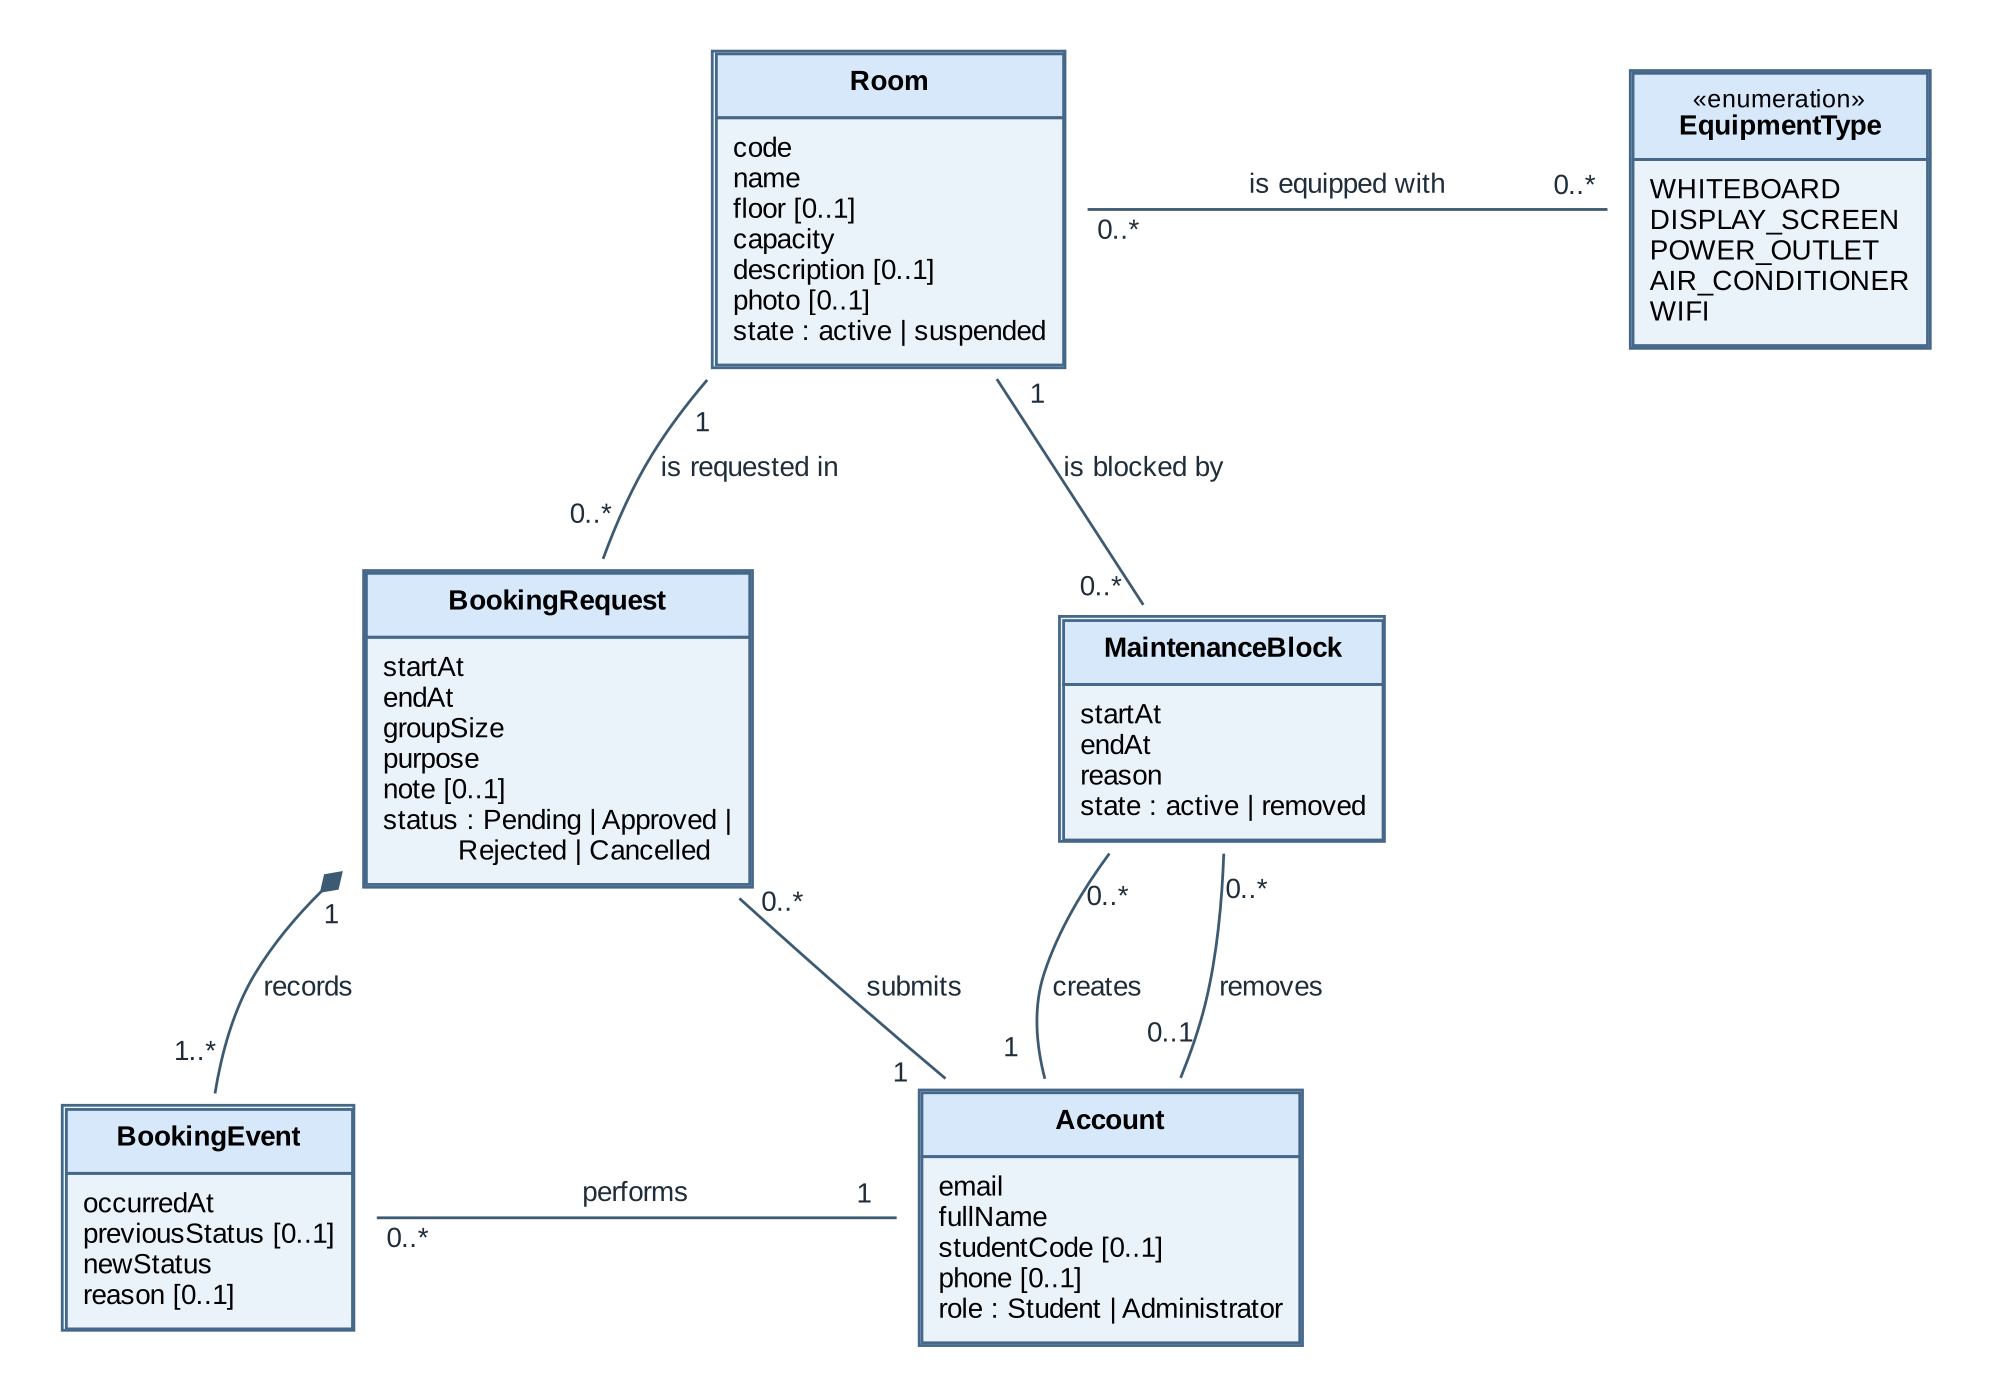
\includegraphics[width=0.94\textwidth,height=0.60\textheight,keepaspectratio]{images/05-object-oriented-design/figure_01.png}
\end{center}
\roomfourfigurecaption{U01}{Conceptual domain model. Attributes name business concepts only; identifiers, foreign keys and operations are deliberately omitted.}
\par\medskip

Role is data, not inheritance. Student and Administrator accounts carry the same identity and profile data and differ only in permissions, which Room4U checks on the server (ADR-003). Only a Student owns requests; only an Administrator creates or removes maintenance blocks and records review transitions.\par

One request, one lifecycle. A BookingRequest becomes a booking when its status is Approved; it is not copied into a second Booking entity (BR-09, BR-12). Each request has one owner and one room; a room receives many requests over time.\par

History is part of the request. BookingEvent is a composition part of its request: one event is created with the request and one for every later status change, and events are never edited or deleted (FR-19, BR-16).\par

Fixed catalogues. Equipment types and purpose codes are fixed ADR-005 catalogues, not records that users manage. A room may have no equipment.\par

Technical data is excluded. room\_occupancy (DB01) is a persistence projection, not a business concept. "Occupies an interval" follows from Approved status or an active block, and "under maintenance" is derived from active blocks rather than stored as a third room state.\par

\subsection{Design class diagrams}

\par\medskip
\begin{center}
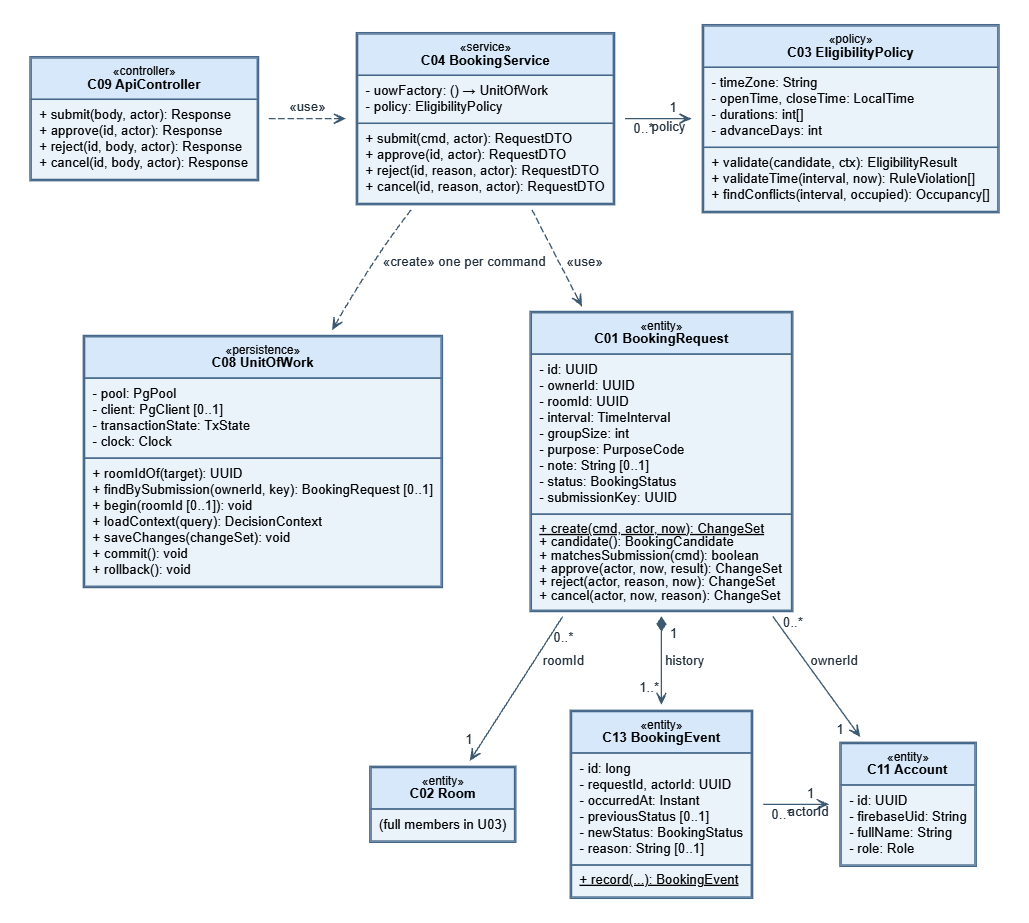
\includegraphics[width=0.94\textwidth,height=0.60\textheight,keepaspectratio]{images/05-object-oriented-design/figure_02.png}
\end{center}
\roomfourfigurecaption{U02}{Booking command package (M04, M06, M07). Services create one UnitOfWork per command; entities stage changes but never execute SQL.}
\par\medskip

C09 passes the server-injected AuthContext; it never reads a role or owner ID from request JSON. C04 holds one shared, stateless C03 and obtains a fresh C08 from its factory for each command. C01 enforces its own transitions and returns a ChangeSet that contains the status change, any occupancy row to add or delete and exactly one C13 event created through record() . Associations to C02 and C11 are ID references (roomId, ownerId), so a command does not need to load a whole object graph.\par

\par\medskip
\begin{center}
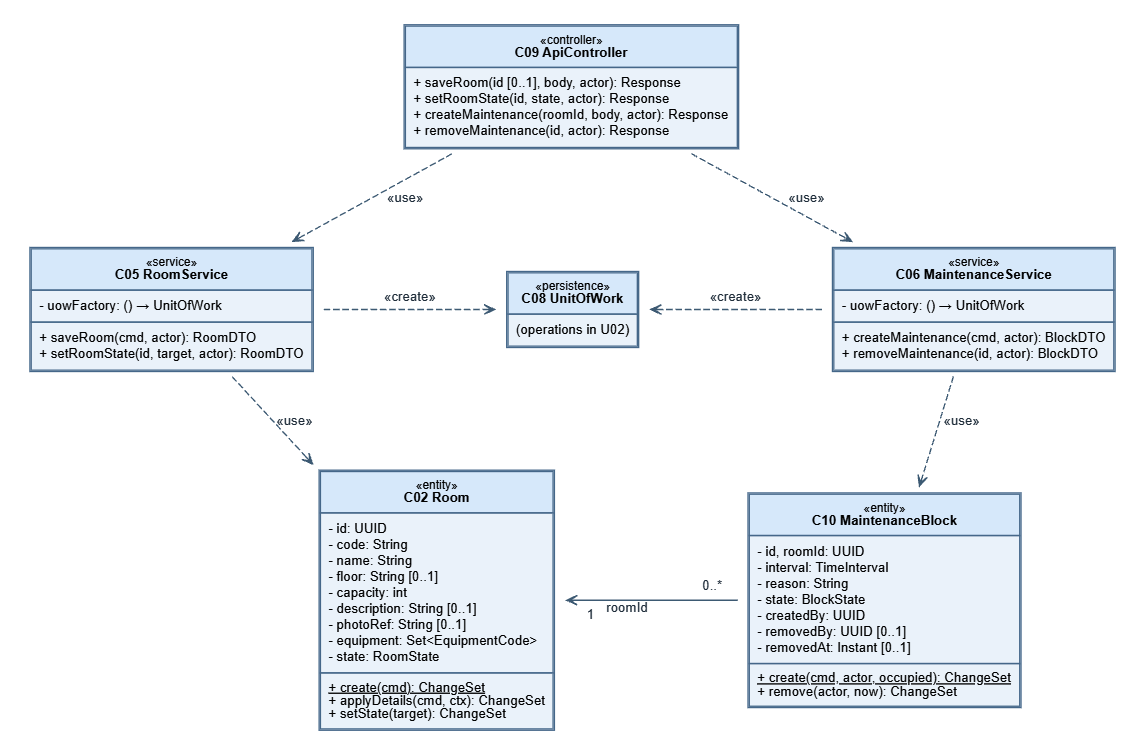
\includegraphics[width=0.94\textwidth,height=0.60\textheight,keepaspectratio]{images/05-object-oriented-design/figure_03.png}
\end{center}
\roomfourfigurecaption{U03}{Room and maintenance command package (M05). C05 and C06 use the same C08 room guard as booking commands.}
\par\medskip

C02.applyDetails receives the decision context read after the room lock: the largest group size among the room's future Approved bookings and whether the normalized code already belongs to another room. C10.create receives the room's current occupancy and refuses any overlap; C10.remove requires an active block whose start is still in the future. Neither service cancels a booking as a side effect.\par

\par\medskip
\begin{center}
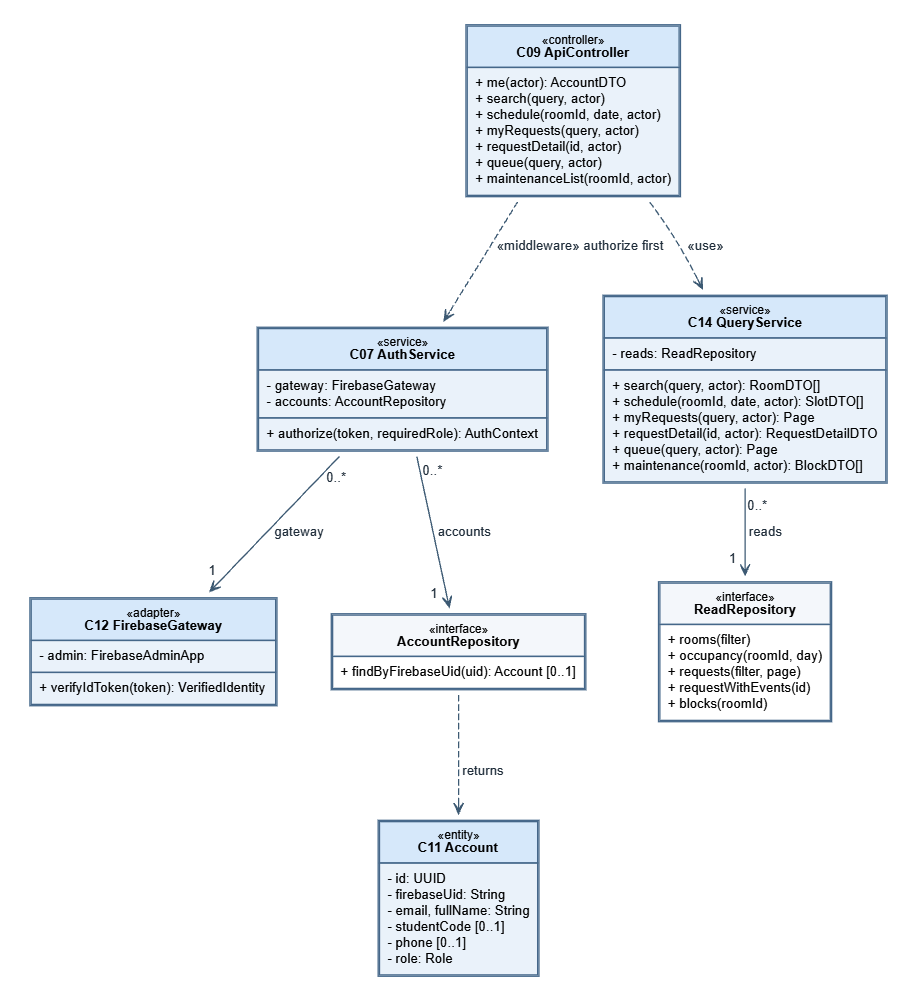
\includegraphics[width=0.94\textwidth,height=0.60\textheight,keepaspectratio]{images/05-object-oriented-design/figure_04.png}
\end{center}
\roomfourfigurecaption{U04}{Access and query package (M01, M03). Authorization runs before dispatch; read services return explicit DTO projections.}
\par\medskip

C09 invokes C07.authorize as middleware before every protected operation. C12 is the only class that imports the Firebase Admin SDK. AccountRepository and ReadRepository are interfaces implemented in the persistence component, so C07 and C14 can be verified with in-memory fakes. C14 checks owner or Administrator access for request details and returns only allow-listed fields; a shared schedule slot contains roomId, startAt, endAt and occupancy type, never an owner or a reason.\par

\subsection{Class specifications}

\subsubsection{C01 BookingRequest}

Domain entity for one student request and its allowed status transitions. No superclass.\par

\small
\setlength{\tabcolsep}{3pt}
\renewcommand{\arraystretch}{1.12}
\begin{longtable}{|p{0.14\textwidth}|p{0.17\textwidth}|p{0.16\textwidth}|p{0.24\textwidth}|p{0.21\textwidth}|}
\hline
\textbf{Attribute} & \textbf{Type} & \textbf{Visibility} & \textbf{Constraint} & \textbf{Description} \\ \hline
\endfirsthead \hline
id & UUID & private & Primary key; immutable & Stable request identity. \\ \hline
ownerId & UUID & private & Student from AuthContext; immutable & Request owner (BR-01). \\ \hline
roomId & UUID & private & Immutable (BR-12) & Requested room; also locates the room guard. \\ \hline
interval & TimeInterval & private & endAt = startAt + duration; never edited & Requested or booked half-open interval. \\ \hline
groupSize & int & private & 1 … room capacity at submission and approval (BR-05) & Number of group members. \\ \hline
purpose & PurposeCode & private & Required; ADR-005 codes & Booking purpose; no eligibility effect. \\ \hline
note & String [0..1] & private & Trimmed; ≤ 250; blank stored as null & Optional booking note. \\ \hline
status & BookingStatus & private & Changed only by the operations below & Lifecycle state. \\ \hline
submissionKey & UUID & private & Unique per owner & Replay key of one logical submission (ADR-004). \\ \hline
createdAt / updatedAt & Instant & private & Server time & Creation order and latest transition. \\ \hline
\end{longtable}
\normalsize

\small
\setlength{\tabcolsep}{3pt}
\renewcommand{\arraystretch}{1.12}
\begin{longtable}{|p{0.18\textwidth}|p{0.24\textwidth}|p{0.22\textwidth}|p{0.28\textwidth}|}
\hline
\textbf{Operation} & \textbf{Parameters → return} & \textbf{Visibility} & \textbf{Responsibility} \\ \hline
\endfirsthead \hline
create (static) & cmd: SubmitCommand, actor, now: Instant → ChangeSet & public & Builds a Pending request and its creation event (previousStatus null). Called only after an eligible C03 result; adds no occupancy (BR-07). \\ \hline
candidate & () → BookingCandidate & public & Returns room, interval and group size for re-validation at approval. \\ \hline
matchesSubmission & cmd: SubmitCommand → boolean & public & Compares the canonical submitted values (room, start, duration, group size, purpose, normalized note) for a replay. \\ \hline
approve & actor, now: Instant, result: EligibilityResult → ChangeSet & public & Requires status Pending and result.eligible. Stages Approved, one occupancy row for (roomId, interval) and one event; otherwise returns a refusal and stages nothing. \\ \hline
reject & actor, reason: String, now: Instant → ChangeSet & public & Administrator; status Pending, also after its start; reason trimmed 1–250 (BR-13). Stages Rejected and an event with the reason. \\ \hline
cancel & actor, now: Instant, reason: String [0..1] → ChangeSet & public & Owner: Pending or Approved and now < startAt. Administrator: Approved, now < startAt and reason 1–250 (BR-10). Stages Cancelled, deletes its own occupancy row when Approved and adds one event. Another student → NOT\_OWNER (403). \\ \hline
\end{longtable}
\normalsize

\subsubsection{C02 Room}

Domain entity for room details, equipment set and active/suspended state. No superclass.\par

\small
\setlength{\tabcolsep}{3pt}
\renewcommand{\arraystretch}{1.12}
\begin{longtable}{|p{0.14\textwidth}|p{0.17\textwidth}|p{0.16\textwidth}|p{0.24\textwidth}|p{0.21\textwidth}|}
\hline
\textbf{Attribute} & \textbf{Type} & \textbf{Visibility} & \textbf{Constraint} & \textbf{Description} \\ \hline
\endfirsthead \hline
id & UUID & private & Stable; immutable & Internal identity, distinct from the editable code. \\ \hline
code & String & private & Trimmed; unique ignoring case (BR-14) & User-facing room code. \\ \hline
name & String & private & Trimmed length 1–80 & Display name. \\ \hline
floor & String [0..1] & private & No fixed enumeration & Floor shown in details and filters. \\ \hline
capacity & int & private & 1–50; ≥ every future Approved group & Current capacity. \\ \hline
description & String [0..1] & private & ≤ 250 characters & Optional description. \\ \hline
photoRef & String [0..1] & private & Preloaded image; null → placeholder & Room photo reference. \\ \hline
equipment & Set<\allowbreak EquipmentCode> & private & ADR-005 codes; may be empty & Selected equipment (room\_equipment rows). \\ \hline
state & RoomState & private & active / suspended & Eligibility gate; not a booking status. \\ \hline
\end{longtable}
\normalsize

\small
\setlength{\tabcolsep}{3pt}
\renewcommand{\arraystretch}{1.12}
\begin{longtable}{|p{0.18\textwidth}|p{0.24\textwidth}|p{0.22\textwidth}|p{0.28\textwidth}|}
\hline
\textbf{Operation} & \textbf{Parameters → return} & \textbf{Visibility} & \textbf{Responsibility} \\ \hline
\endfirsthead \hline
create (static) & cmd: RoomCommand → ChangeSet & public & Validates fields and codes, assigns a new stable ID and stages an active room with its equipment rows (FR-20). The normalized unique index rejects a duplicate code at save. \\ \hline
applyDetails & cmd: RoomCommand, ctx: DecisionContext → ChangeSet & public & Validates fields; refuses a code used by another room (ctx.codeInUse) or capacity < ctx.maxFutureGroup (BR-14). Stages the detail update and, when supplied, replaces the whole equipment set. The ID never changes (FR-21). \\ \hline
setState & target: RoomState → ChangeSet & public & Allows only active → suspended and suspended → active. Never changes bookings, blocks or occupancy (BR-11). \\ \hline
\end{longtable}
\normalsize

\subsubsection{C03 EligibilityPolicy}

Stateless implementation of UC-14 used by submission and approval. It reads only the supplied context and never writes. No superclass.\par

\small
\setlength{\tabcolsep}{3pt}
\renewcommand{\arraystretch}{1.12}
\begin{longtable}{|p{0.14\textwidth}|p{0.17\textwidth}|p{0.16\textwidth}|p{0.24\textwidth}|p{0.21\textwidth}|}
\hline
\textbf{Attribute} & \textbf{Type} & \textbf{Visibility} & \textbf{Constraint} & \textbf{Description} \\ \hline
\endfirsthead \hline
timeZone & String & private & Asia/Ho\_Chi\_Minh & Local date and opening-hour interpretation. \\ \hline
openTime / closeTime & LocalTime & private & 08:00 / 20:00 & Booking window on one local date (BR-02). \\ \hline
durations & int[] & private & \{30, 60, 90, 120\} & Allowed durations in minutes (BR-03). \\ \hline
startStep\allowbreak Minutes & int & private & 30 & Start on :00 or :30 with zero seconds. \\ \hline
advanceDays & int & private & 7; rolling instant boundary & Maximum advance period (BR-04). \\ \hline
\end{longtable}
\normalsize

\small
\setlength{\tabcolsep}{3pt}
\renewcommand{\arraystretch}{1.12}
\begin{longtable}{|p{0.18\textwidth}|p{0.24\textwidth}|p{0.22\textwidth}|p{0.28\textwidth}|}
\hline
\textbf{Operation} & \textbf{Parameters → return} & \textbf{Visibility} & \textbf{Responsibility} \\ \hline
\endfirsthead \hline
validate & candidate: BookingCandidate, ctx: DecisionContext → EligibilityResult & public & Collects all violations: room active (BR-11), validateTime, 1 ≤ groupSize ≤ ctx room capacity (BR-05) and no conflict from findConflicts (BR-06–08). \\ \hline
validateTime & interval: TimeInterval, now: Instant → RuleViolation[] & public & Start step, allowed duration, same local date inside 08:00–20:00 (end at 20:00 allowed) and now < start ≤ now + 7 days. \\ \hline
findConflicts & interval: TimeInterval, occupied: Occupancy[] → Occupancy[] & public & Returns Approved or maintenance occupancy that overlaps the interval. Pending requests are never in occupied (BR-07). \\ \hline
\end{longtable}
\normalsize

\subsubsection{C04 BookingService}

Coordinates submission, approval, rejection and cancellation (UC-04, UC-06, UC-08–UC-10). No superclass.\par

\small
\setlength{\tabcolsep}{3pt}
\renewcommand{\arraystretch}{1.12}
\begin{longtable}{|p{0.14\textwidth}|p{0.17\textwidth}|p{0.16\textwidth}|p{0.24\textwidth}|p{0.21\textwidth}|}
\hline
\textbf{Attribute} & \textbf{Type} & \textbf{Visibility} & \textbf{Constraint} & \textbf{Description} \\ \hline
\endfirsthead \hline
uowFactory & () → UnitOfWork & private & New unit per command & Never shares a transaction client between requests. \\ \hline
policy & EligibilityPolicy & private & Injected; shared; stateless & UC-14 rules. \\ \hline
\end{longtable}
\normalsize

\small
\setlength{\tabcolsep}{3pt}
\renewcommand{\arraystretch}{1.12}
\begin{longtable}{|p{0.18\textwidth}|p{0.24\textwidth}|p{0.22\textwidth}|p{0.28\textwidth}|}
\hline
\textbf{Operation} & \textbf{Parameters → return} & \textbf{Visibility} & \textbf{Responsibility} \\ \hline
\endfirsthead \hline
submit & cmd: SubmitCommand, actor → RequestDTO & public & Student. Replay check by owner/key (200 same values, 409 different). If no request is found, lock the room and repeat the owner/key lookup before running UC-14; a hit rolls back and is answered as a replay. Otherwise load ctx, validate, C01.create, save and commit → 201 Pending. A unique-key conflict at save rolls back, rereads the stored request and is answered as a replay. \\ \hline
approve & id: UUID, actor → RequestDTO & public & Administrator. roomIdOf, lock, reload request and occupancy, validate, C01.approve, save, commit. Request no longer Pending → rollback, 409 with its current status. Pending but not eligible, or an exclusion violation (23P01) → rollback, 409 with the causes; the request stays Pending. \\ \hline
reject & id: UUID, reason: String, actor → RequestDTO & public & Administrator. Same guard; C01.reject; no occupancy change. \\ \hline
cancel & id: UUID, reason: String [0..1], actor → RequestDTO & public & Owner (UC-06) or Administrator (UC-10). Same guard; C01.cancel; releases only this request's occupancy. \\ \hline
\end{longtable}
\normalsize

\subsubsection{C05 RoomService}

Creates and edits rooms and changes room state (UC-11, UC-12). No superclass.\par

\small
\setlength{\tabcolsep}{3pt}
\renewcommand{\arraystretch}{1.12}
\begin{longtable}{|p{0.14\textwidth}|p{0.17\textwidth}|p{0.16\textwidth}|p{0.24\textwidth}|p{0.21\textwidth}|}
\hline
\textbf{Attribute} & \textbf{Type} & \textbf{Visibility} & \textbf{Constraint} & \textbf{Description} \\ \hline
\endfirsthead \hline
uowFactory & () → UnitOfWork & private & New unit per command & Transaction and room guard. \\ \hline
\end{longtable}
\normalsize

\small
\setlength{\tabcolsep}{3pt}
\renewcommand{\arraystretch}{1.12}
\begin{longtable}{|p{0.18\textwidth}|p{0.24\textwidth}|p{0.22\textwidth}|p{0.28\textwidth}|}
\hline
\textbf{Operation} & \textbf{Parameters → return} & \textbf{Visibility} & \textbf{Responsibility} \\ \hline
\endfirsthead \hline
saveRoom & cmd: RoomCommand, actor → RoomDTO & public & Administrator. New room: begin(null), C02.create, save, commit; duplicate normalized code (23505) → 409. Existing room: begin(roomId), loadContext, C02.applyDetails, save, commit (SQ04). \\ \hline
setRoomState & id: UUID, target: RoomState, actor → RoomDTO & public & Administrator. begin(id), reread state, C02.setState, save, commit. Existing bookings and blocks stay unchanged. \\ \hline
\end{longtable}
\normalsize

\subsubsection{C06 MaintenanceService}

Creates maintenance blocks and removes future blocks (UC-13). No superclass.\par

\small
\setlength{\tabcolsep}{3pt}
\renewcommand{\arraystretch}{1.12}
\begin{longtable}{|p{0.14\textwidth}|p{0.17\textwidth}|p{0.16\textwidth}|p{0.24\textwidth}|p{0.21\textwidth}|}
\hline
\textbf{Attribute} & \textbf{Type} & \textbf{Visibility} & \textbf{Constraint} & \textbf{Description} \\ \hline
\endfirsthead \hline
uowFactory & () → UnitOfWork & private & New unit per command & Same room guard as approval. \\ \hline
\end{longtable}
\normalsize

\small
\setlength{\tabcolsep}{3pt}
\renewcommand{\arraystretch}{1.12}
\begin{longtable}{|p{0.18\textwidth}|p{0.24\textwidth}|p{0.22\textwidth}|p{0.28\textwidth}|}
\hline
\textbf{Operation} & \textbf{Parameters → return} & \textbf{Visibility} & \textbf{Responsibility} \\ \hline
\endfirsthead \hline
createMaintenance & cmd: BlockCommand, actor → BlockDTO & public & Administrator. begin(roomId), load occupancy, C10.create, save, commit. On overlap, roll back and return 409 with code SCHEDULE\_CONFLICT, requestId and conflicts. Following SQ05, list overlapping Approved bookings first (kind = approved\_booking, bookingRequestId, startAt, endAt); only if none overlap, return the active maintenance conflict (kind = maintenance\_block, maintenanceBlockId, startAt, endAt). S08 links bookings to UC-10; no booking is cancelled automatically (BR-15). \\ \hline
removeMaintenance & id: UUID, actor → BlockDTO & public & Administrator. roomIdOf(block), begin, reload block, C10.remove(actor, ctx.now), save, commit. The block record is kept (FR-26). \\ \hline
\end{longtable}
\normalsize

\subsubsection{C07 AuthService}

Verifies identity and resolves the application role before any protected behavior. No superclass.\par

\small
\setlength{\tabcolsep}{3pt}
\renewcommand{\arraystretch}{1.12}
\begin{longtable}{|p{0.14\textwidth}|p{0.17\textwidth}|p{0.16\textwidth}|p{0.24\textwidth}|p{0.21\textwidth}|}
\hline
\textbf{Attribute} & \textbf{Type} & \textbf{Visibility} & \textbf{Constraint} & \textbf{Description} \\ \hline
\endfirsthead \hline
gateway & FirebaseGateway & private & Adapter over Firebase Admin SDK & Verifies ID tokens. \\ \hline
accounts & AccountRepository & private & Read-only & Maps firebaseUid to the internal account and role. \\ \hline
\end{longtable}
\normalsize

\small
\setlength{\tabcolsep}{3pt}
\renewcommand{\arraystretch}{1.12}
\begin{longtable}{|p{0.18\textwidth}|p{0.24\textwidth}|p{0.22\textwidth}|p{0.28\textwidth}|}
\hline
\textbf{Operation} & \textbf{Parameters → return} & \textbf{Visibility} & \textbf{Responsibility} \\ \hline
\endfirsthead \hline
authorize & token: String, requiredRole: Role [0..1] → AuthContext & public & Invalid or expired token, or no matching account → 401; role differs from requiredRole → 403. Returns only \{userId, role\} from the users row. Runs before dispatch, so no Firebase call happens while a room lock is held. \\ \hline
\end{longtable}
\normalsize

\subsubsection{C08 UnitOfWork}

One-command transaction and repository facade (M07). Each instance owns at most one pooled client. No superclass.\par

\small
\setlength{\tabcolsep}{3pt}
\renewcommand{\arraystretch}{1.12}
\begin{longtable}{|p{0.14\textwidth}|p{0.17\textwidth}|p{0.16\textwidth}|p{0.24\textwidth}|p{0.21\textwidth}|}
\hline
\textbf{Attribute} & \textbf{Type} & \textbf{Visibility} & \textbf{Constraint} & \textbf{Description} \\ \hline
\endfirsthead \hline
pool & PgPool & private & Configured once per process & Connection source; not the transaction itself. \\ \hline
client & PgClient [0..1] & private & One checked-out connection until commit/rollback & Every statement of the command uses this client. \\ \hline
transaction\allowbreak State & TxState & private & idle / active / committed / rolledBack & Blocks writes outside an active unit. \\ \hline
clock & Clock & private & Server clock in production; fixed clock in tests & Decision instant sampled after the lock. \\ \hline
\end{longtable}
\normalsize

\small
\setlength{\tabcolsep}{3pt}
\renewcommand{\arraystretch}{1.12}
\begin{longtable}{|p{0.18\textwidth}|p{0.24\textwidth}|p{0.22\textwidth}|p{0.28\textwidth}|}
\hline
\textbf{Operation} & \textbf{Parameters → return} & \textbf{Visibility} & \textbf{Responsibility} \\ \hline
\endfirsthead \hline
roomIdOf & target: TargetRef → UUID & public & Non-locking read of the immutable room\_id of a request or block before BEGIN; unknown target → 404. \\ \hline
findBySubmission & ownerId: UUID, key: UUID → BookingRequest [0..1] & public & Replay lookup by owner and key. Called before the submission transaction, again after the room guard is held, and after a rollback caused by a unique-key conflict. \\ \hline
begin & roomId: UUID [0..1] → void & public & BEGIN at READ COMMITTED and SELECT the rooms row FOR UPDATE. Null only for creating a new room. \\ \hline
loadContext & query: ContextQuery → DecisionContext & public & Reads current room, target, occupancy, maxFutureGroup and codeInUse as the query requests; samples now (clock\_timestamp) after the lock. \\ \hline
saveChanges & changeSet: ChangeSet → void & public & Writes source rows, occupancy projection and events with the same client. Maps 23P01 to a schedule conflict and 23505 by constraint name. \\ \hline
commit & () → void & public & COMMIT and release the client; services report success only afterwards. \\ \hline
rollback & () → void & public & ROLLBACK and release the client after any refusal or error; safe to call twice. \\ \hline
\end{longtable}
\normalsize

\subsubsection{Supporting classes C09–C14}

\small
\setlength{\tabcolsep}{2pt}
\renewcommand{\arraystretch}{1.12}
\begin{longtable}{|>{\raggedright\arraybackslash}p{0.18\textwidth}|>{\raggedright\arraybackslash}p{0.24\textwidth}|>{\raggedright\arraybackslash}p{0.22\textwidth}|>{\raggedright\arraybackslash}p{0.28\textwidth}|}
\hline
\textbf{ID} & \textbf{Class} & \textbf{Responsibility} & \textbf{Key operations} \\ \hline
\endfirsthead \hline
C09 & ApiController\allowbreak{} «controller» & Routes /api/v1, parses DTOs, runs C07 as middleware, translates domain outcomes to 401/\allowbreak 403/\allowbreak 404/\allowbreak 409/\allowbreak 422/\allowbreak 503. & As listed in U02–U04. \\ \hline
C10 & MaintenanceBlock «entity» & Block interval, reason, active/removed state, creator and remover. Removed blocks are retained. & create (static): end > start, reason trimmed 1–250, no overlap with occupied → block + occupancy (BR-13, BR-15). remove(actor, now): active and now < startAt → removed, delete own occupancy, record actor and time (FR-26). \\ \hline
C11 & Account «entity» & Pre-created account with profile fields and role; read-only in this scope. & Attributes only. \\ \hline
C12 & FirebaseGateway «adapter» & Only class that depends on the Firebase Admin SDK. & verifyIdToken(token) → VerifiedIdentity. \\ \hline
C13 & BookingEvent «entity» & Append-only transition record; never updated or deleted. & record (static): event for a creation or transition. \\ \hline
C14 & QueryService «service» & Read use cases UC-03, UC-05, UC-07 and the S08 block list through ReadRepository; owner/Administrator checks; paging. & search, schedule, myRequests, requestDetail, queue, maintenance. \\ \hline
\end{longtable}
\normalsize

\subsection{Sequence diagrams}

SQ01–SQ05 show five Must flows; arrows mark calls/returns and alt fragments show PA2 alternatives/errors. Section 4.8 defines C09 routes, C07 authorizes, and Section 4.6 governs commit/rollback.\par

\clearpage
\subsubsection{SQ01 UC-04 Submit booking request}

\begin{center}
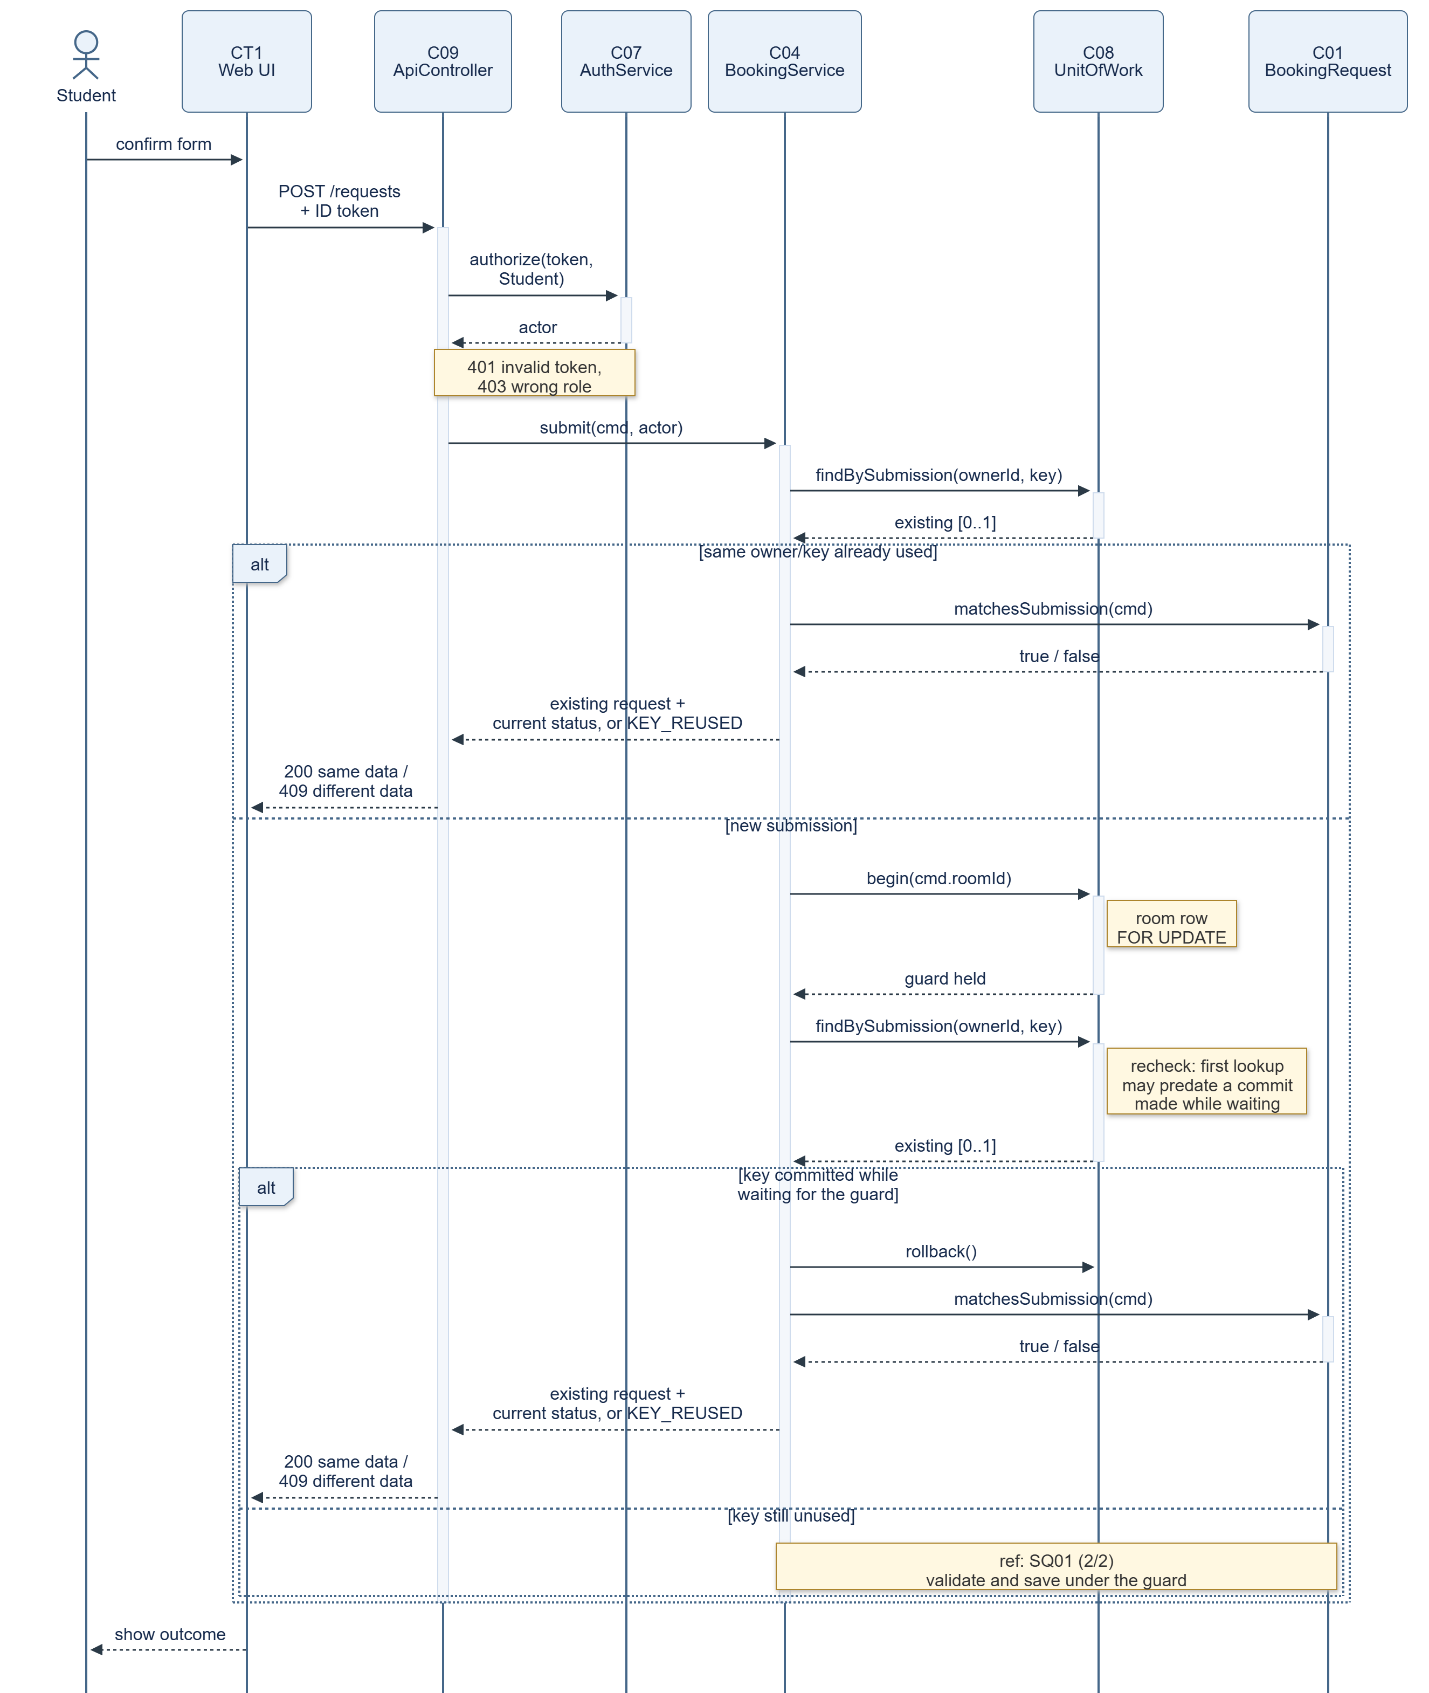
\includegraphics[width=0.98\textwidth,height=0.84\textheight,keepaspectratio]{images/05-object-oriented-design/figure_05.png}
\end{center}
\roomfourfigurecaption{SQ01a}{UC-04 submission, part 1 of 2: authorization, initial replay lookup and room-guard recheck.}

\clearpage
\begin{center}
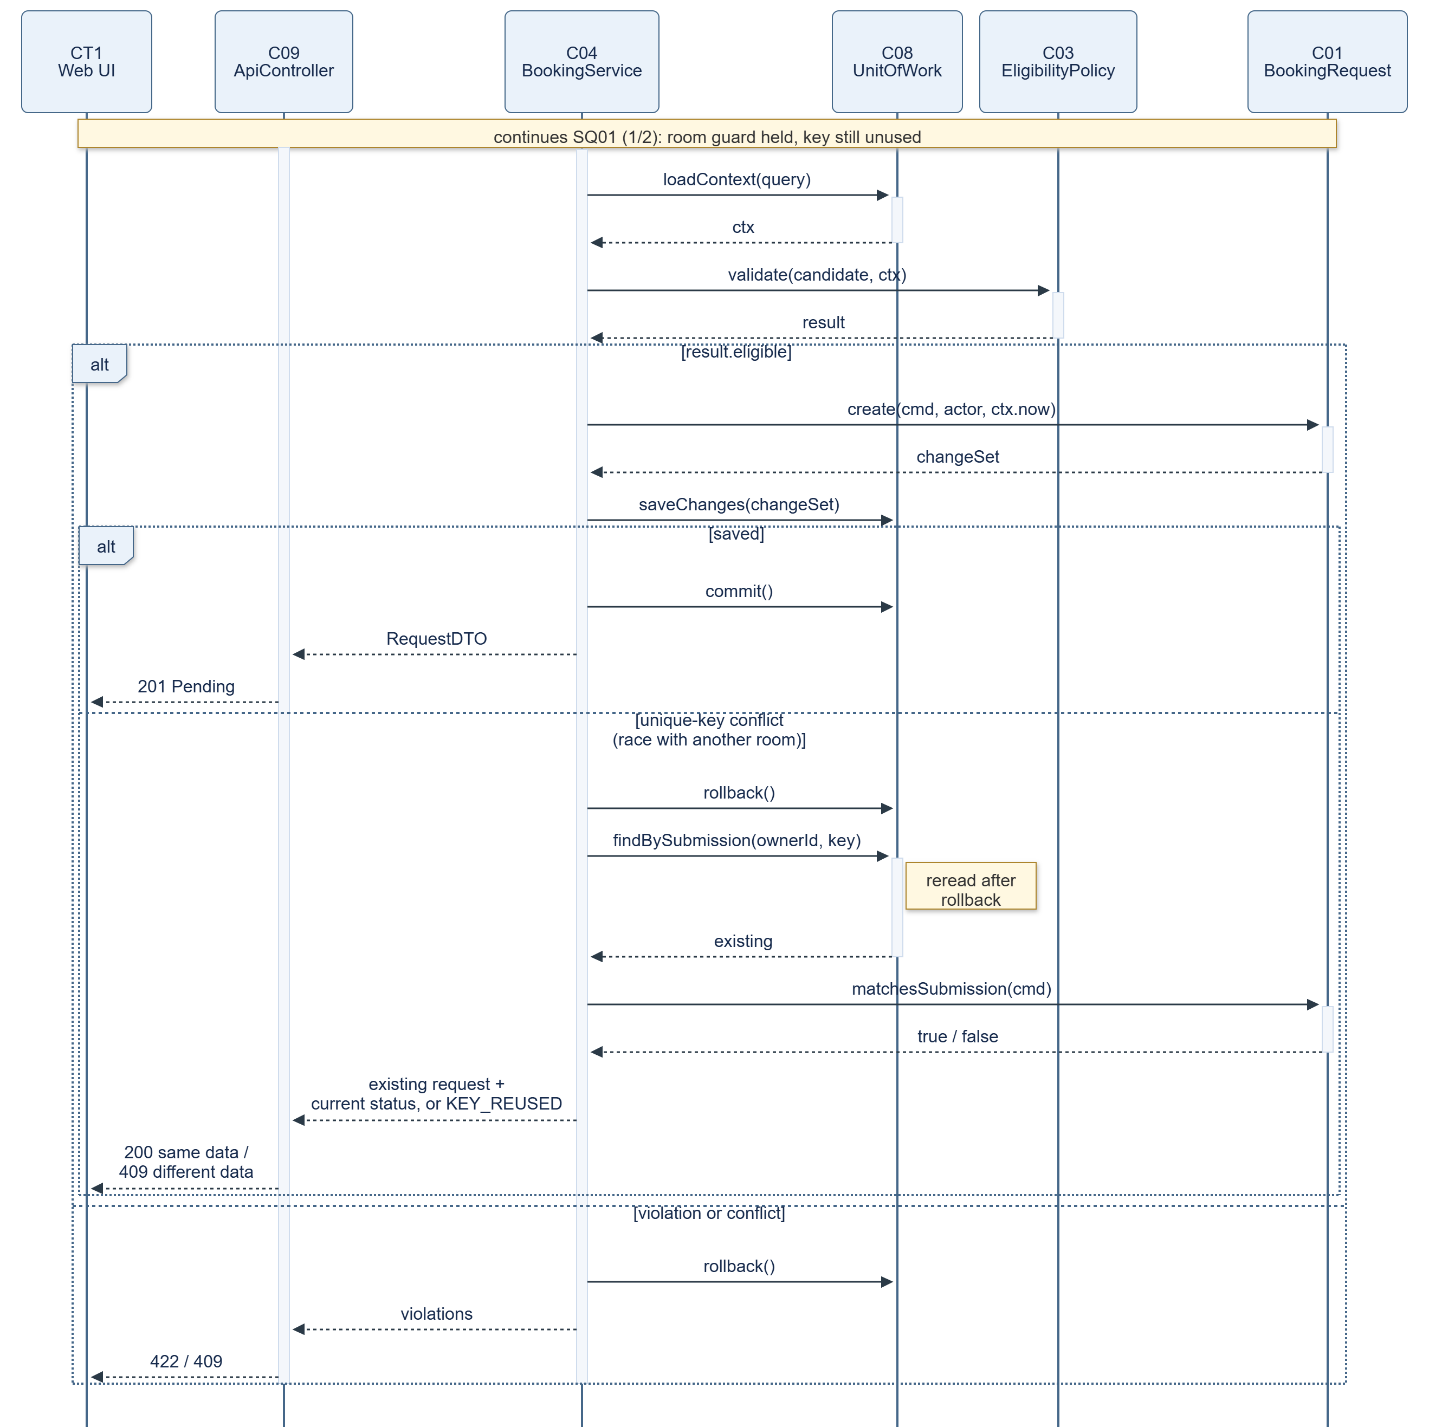
\includegraphics[width=0.98\textwidth,height=0.84\textheight,keepaspectratio]{images/05-object-oriented-design/figure_06.png}
\end{center}
\roomfourfigurecaption{SQ01b}{UC-04 submission, part 2 of 2: validation, commit and unique-key conflict handling.}
\clearpage

The replay branch runs first: the same owner and submissionKey return the existing request (200) when the canonical values match and 409 when they differ. If the first lookup finds no request, the service takes the room guard and looks up ownerId + submissionKey again before running UC-14, because a submission with the same key may have committed while this one was waiting for the guard; a hit rolls back and is answered as a replay. Only when the key is still unused does query load the locked room and its occupancy. The successful ChangeSet contains the Pending request and its creation event, with no occupancy row; overlapping Pending requests are not occupancy and never block a submission (BR-07). Field violations return 422; a suspended room or an occupied interval returns 409. A same-key submission for another room is not serialized by this guard, so the unique constraint on ownerId + submissionKey can still fail at saveChanges; the service then rolls back, rereads the stored request and handles it as a replay (200 or 409).\par

\subsubsection{SQ02 UC-08 approval}

\par\medskip
\begin{center}
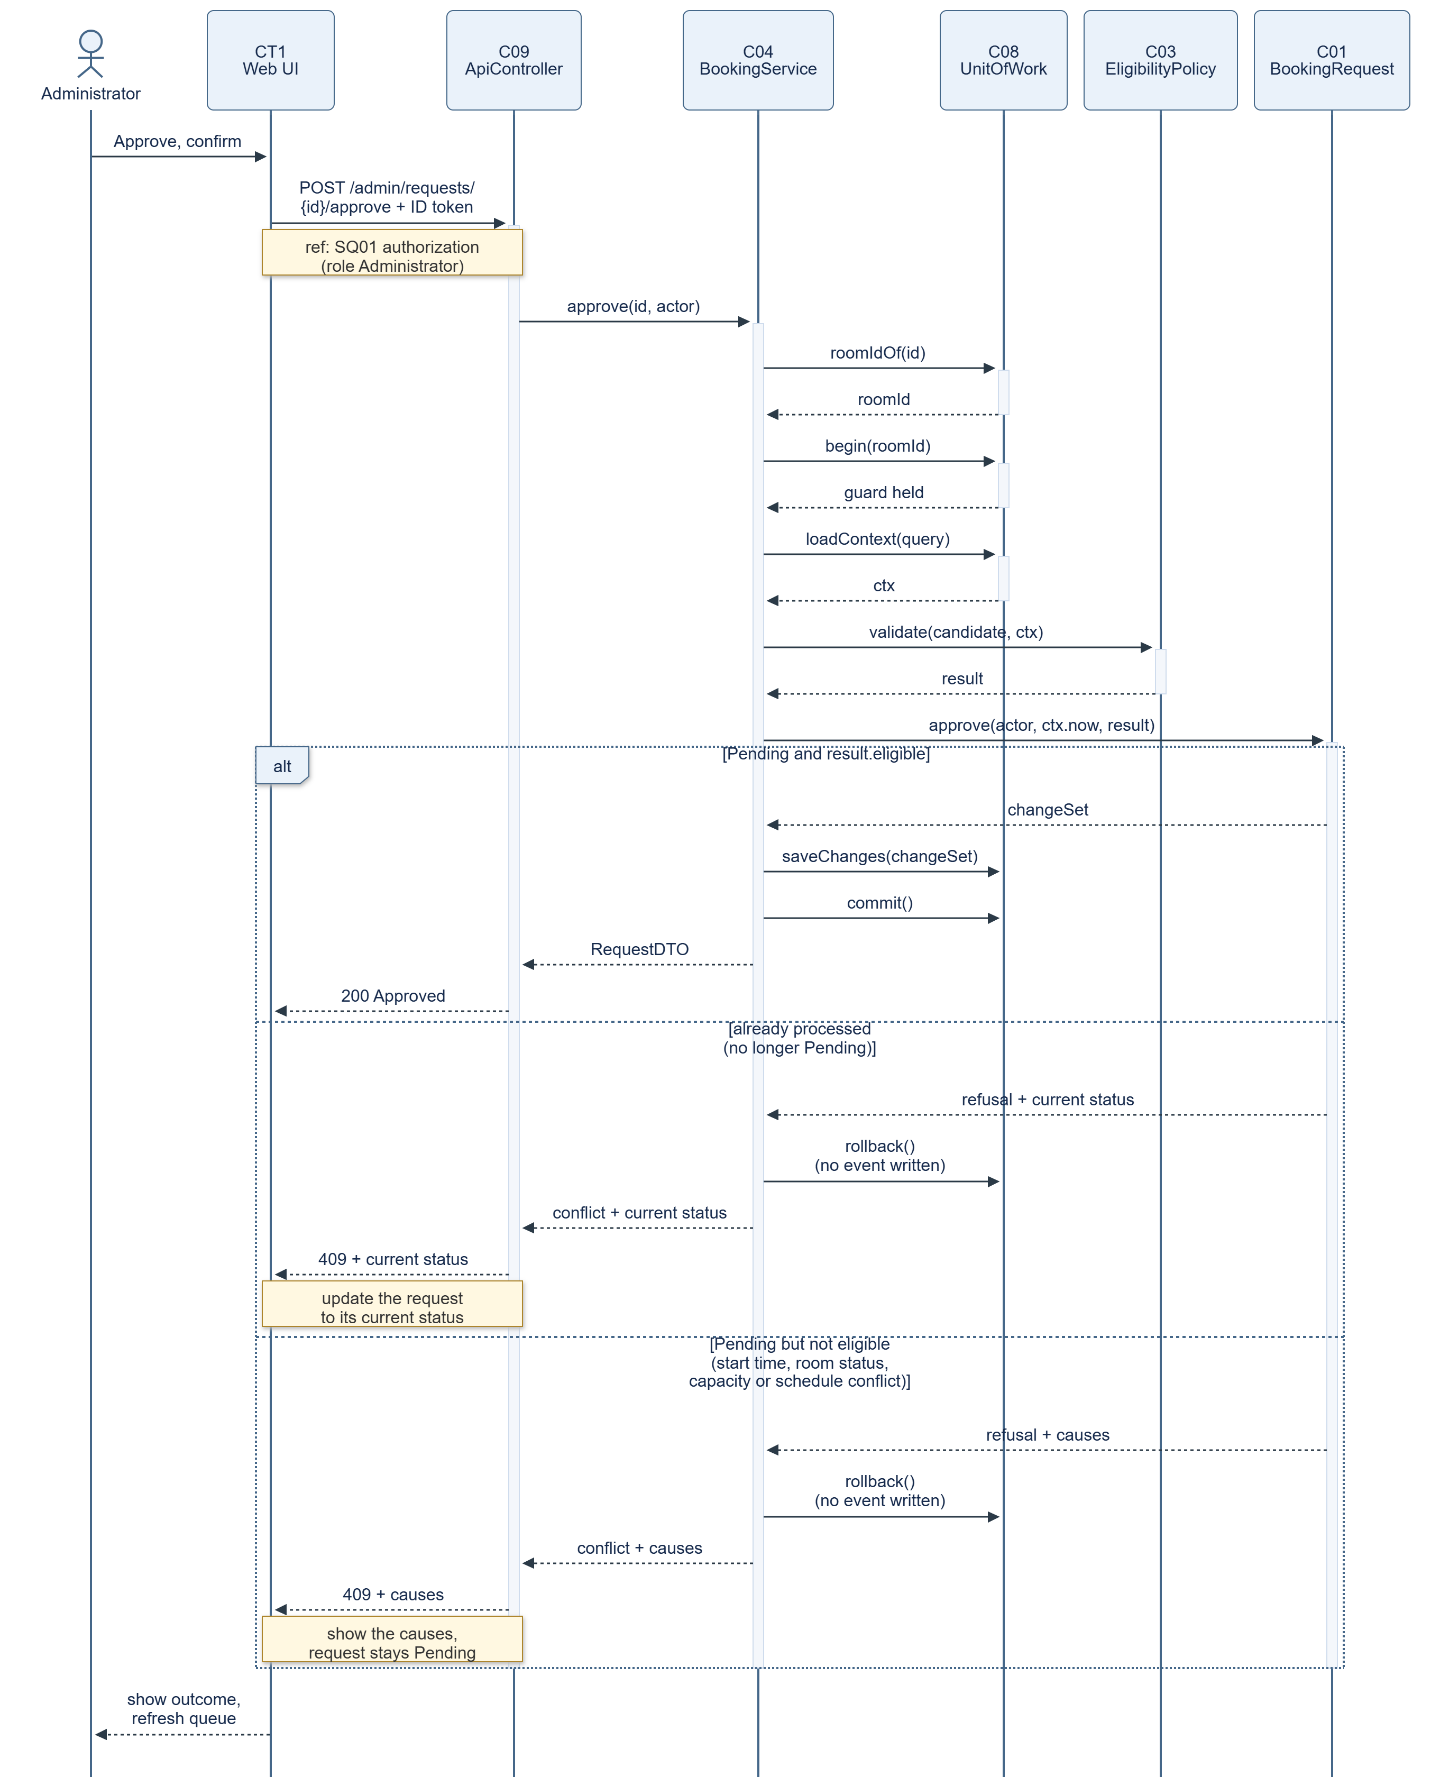
\includegraphics[width=0.94\textwidth,height=0.60\textheight,keepaspectratio]{images/05-object-oriented-design/figure_07.png}
\end{center}
\roomfourfigurecaption{SQ02}{UC-08 approval with eligibility re-evaluated after the room guard.}
\par\medskip

The service resolves the immutable room ID, takes the room guard and only then reads the request, room and occupancy. C03 rechecks time against the decision instant (BR-04 at approval), suspension, capacity and overlap; C01.approve additionally requires status Pending. The ChangeSet stages Approved, exactly one matching occupancy row and one event. A refusal has two outcomes, and neither writes an event. If the request has already been processed (approved, rejected or cancelled in the meantime), the service rolls back and returns 409 with its current status so that the UI shows that status. If the request is still Pending but not eligible, for example because a concurrent approval or maintenance command committed first and its occupancy is visible after the lock, the service rolls back and returns 409 with the causes, and the request stays Pending. The exclusion constraint (23P01) is the last safeguard and is reported as a schedule conflict in the same way. UC-09 rejection uses the same frame with C01.reject and no C03 call.\par

\subsubsection{SQ03 UC-06 Cancel own request}

\par\medskip
\begin{center}
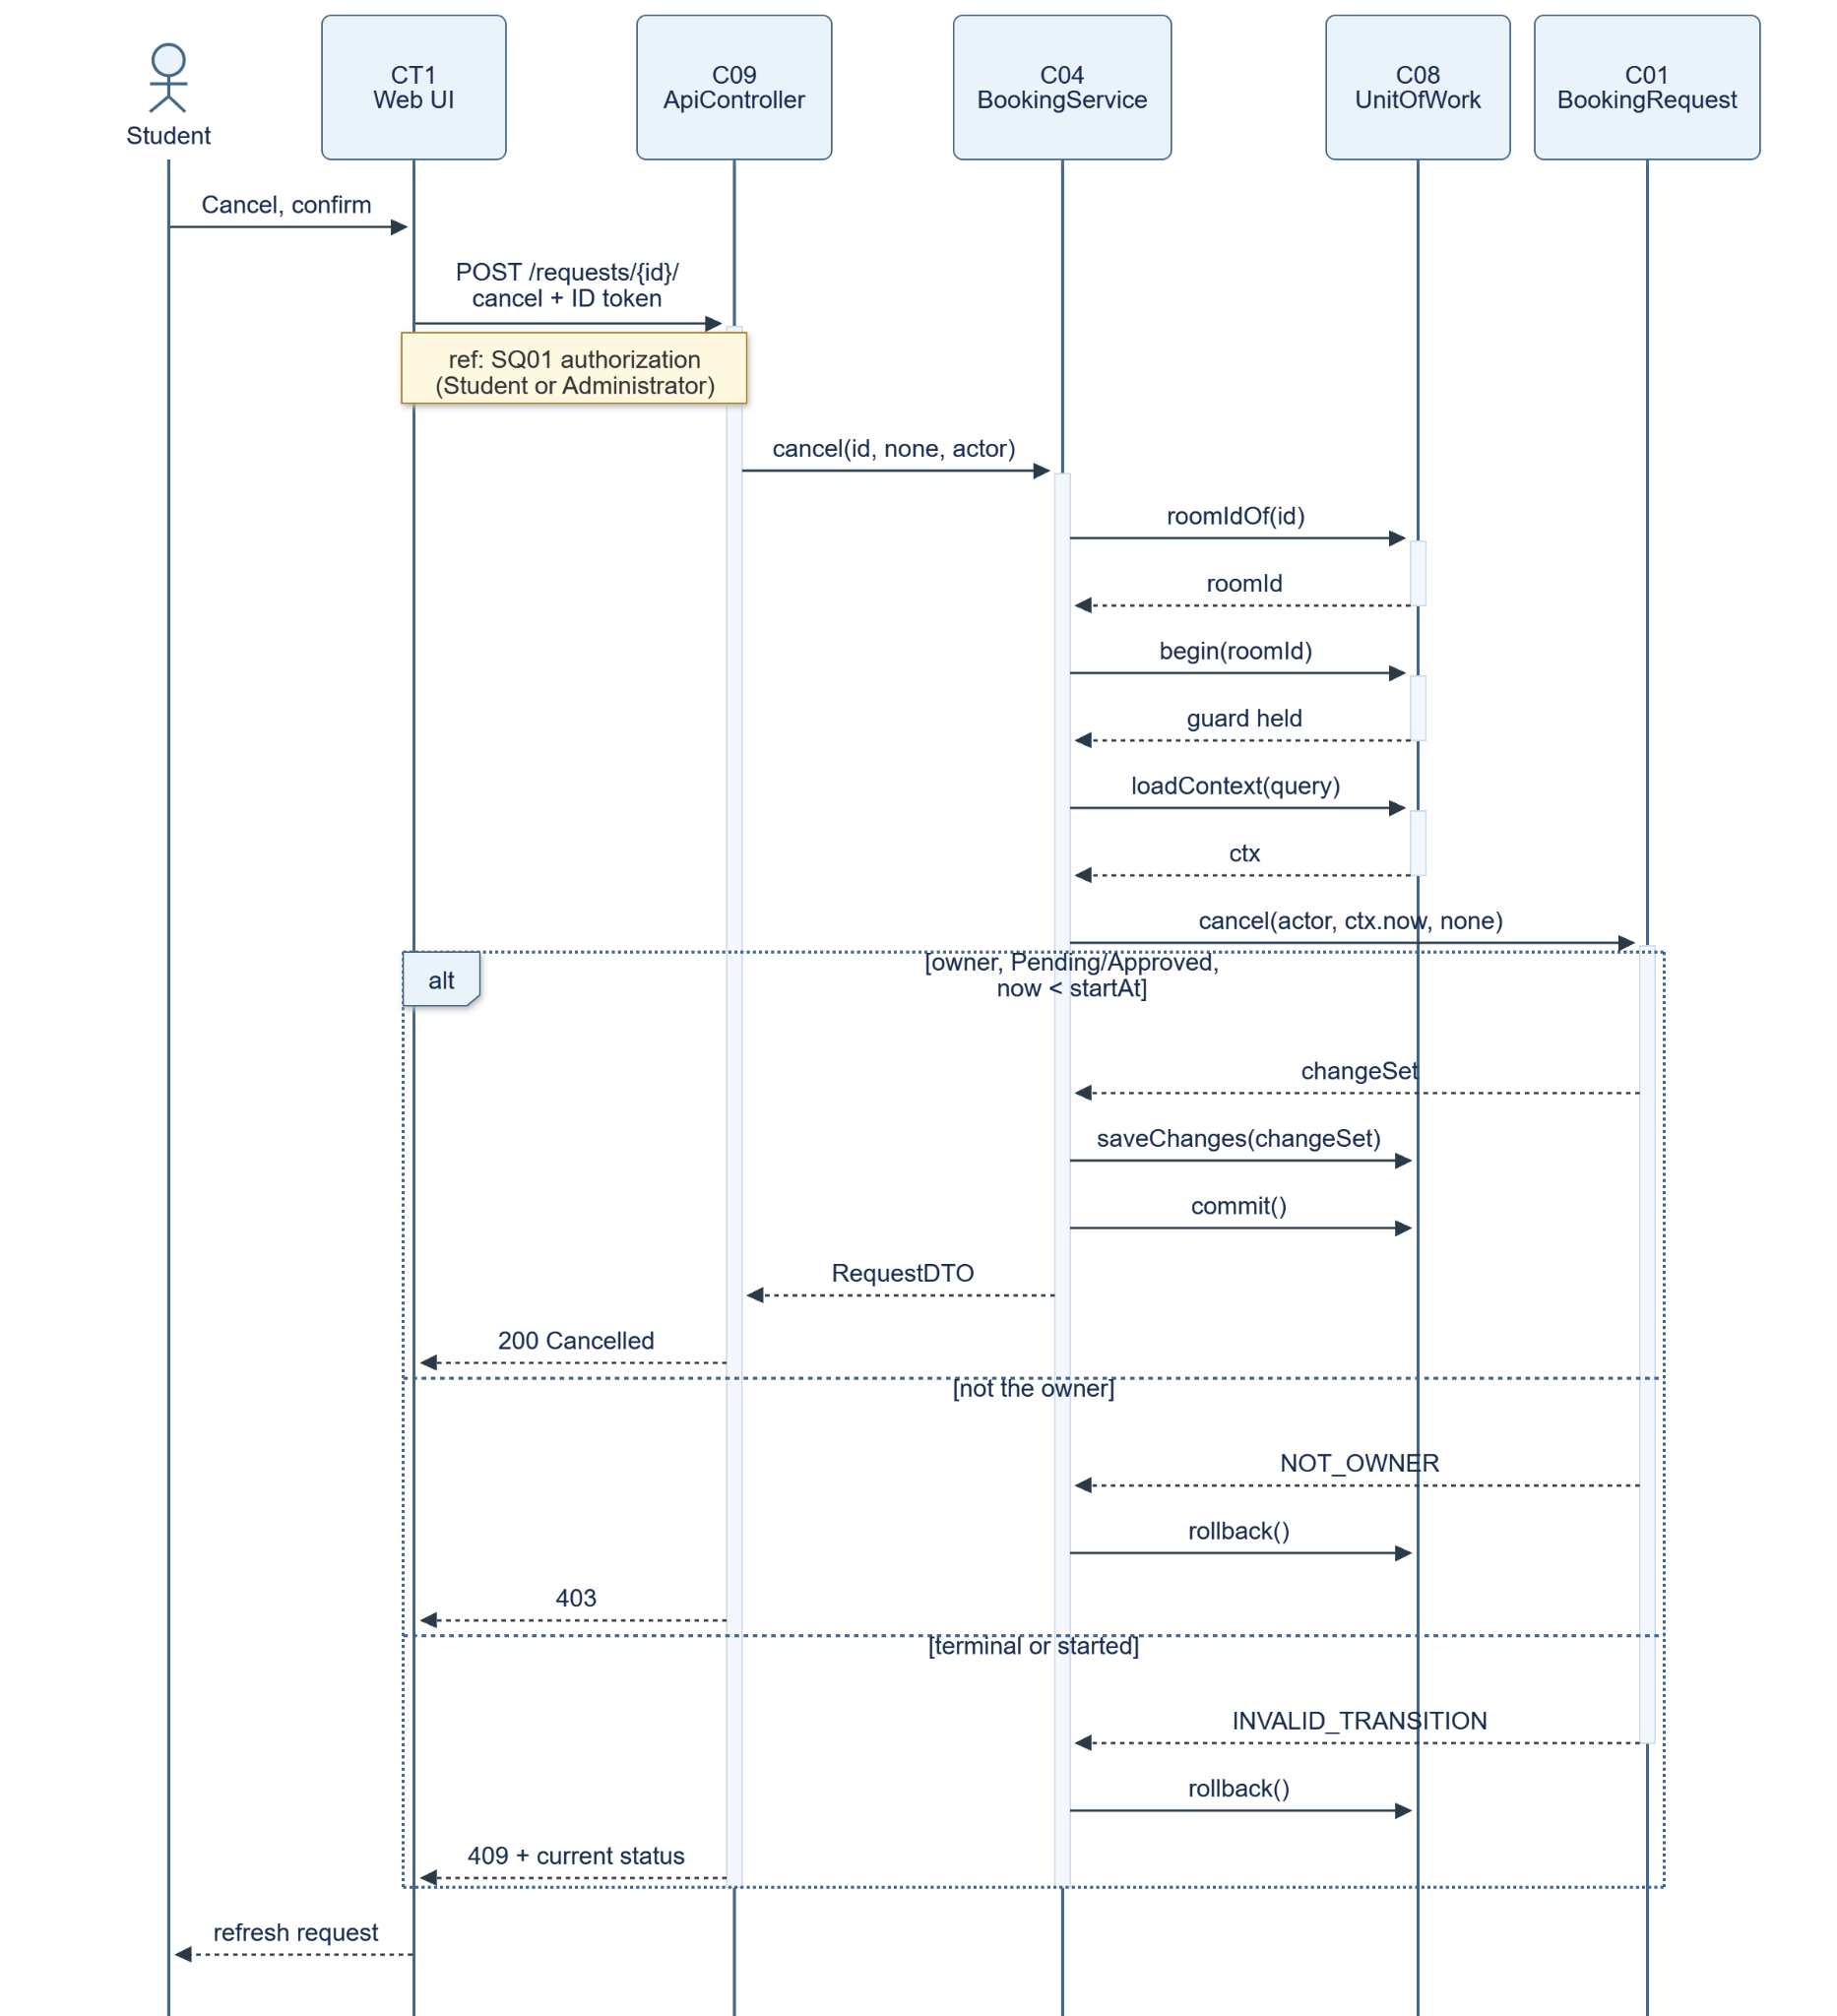
\includegraphics[width=0.94\textwidth,height=0.60\textheight,keepaspectratio]{images/05-object-oriented-design/figure_08.png}
\end{center}
\roomfourfigurecaption{SQ03}{UC-06 owner cancellation; UC-10 reuses the same operation for an Administrator.}
\par\medskip

C01.cancel checks the server-derived actor, the current status and now < startAt using ctx.now. Cancelling an Approved request deletes only its own occupancy row. A request owned by another student returns 403 without record data; a Rejected, Cancelled or started request returns 409 with its current status. UC-10 calls the same operation with an Administrator actor, which is limited to Approved bookings and requires a reason.\par

\subsubsection{SQ04 UC-11 Edit room details}

\par\medskip
\begin{center}
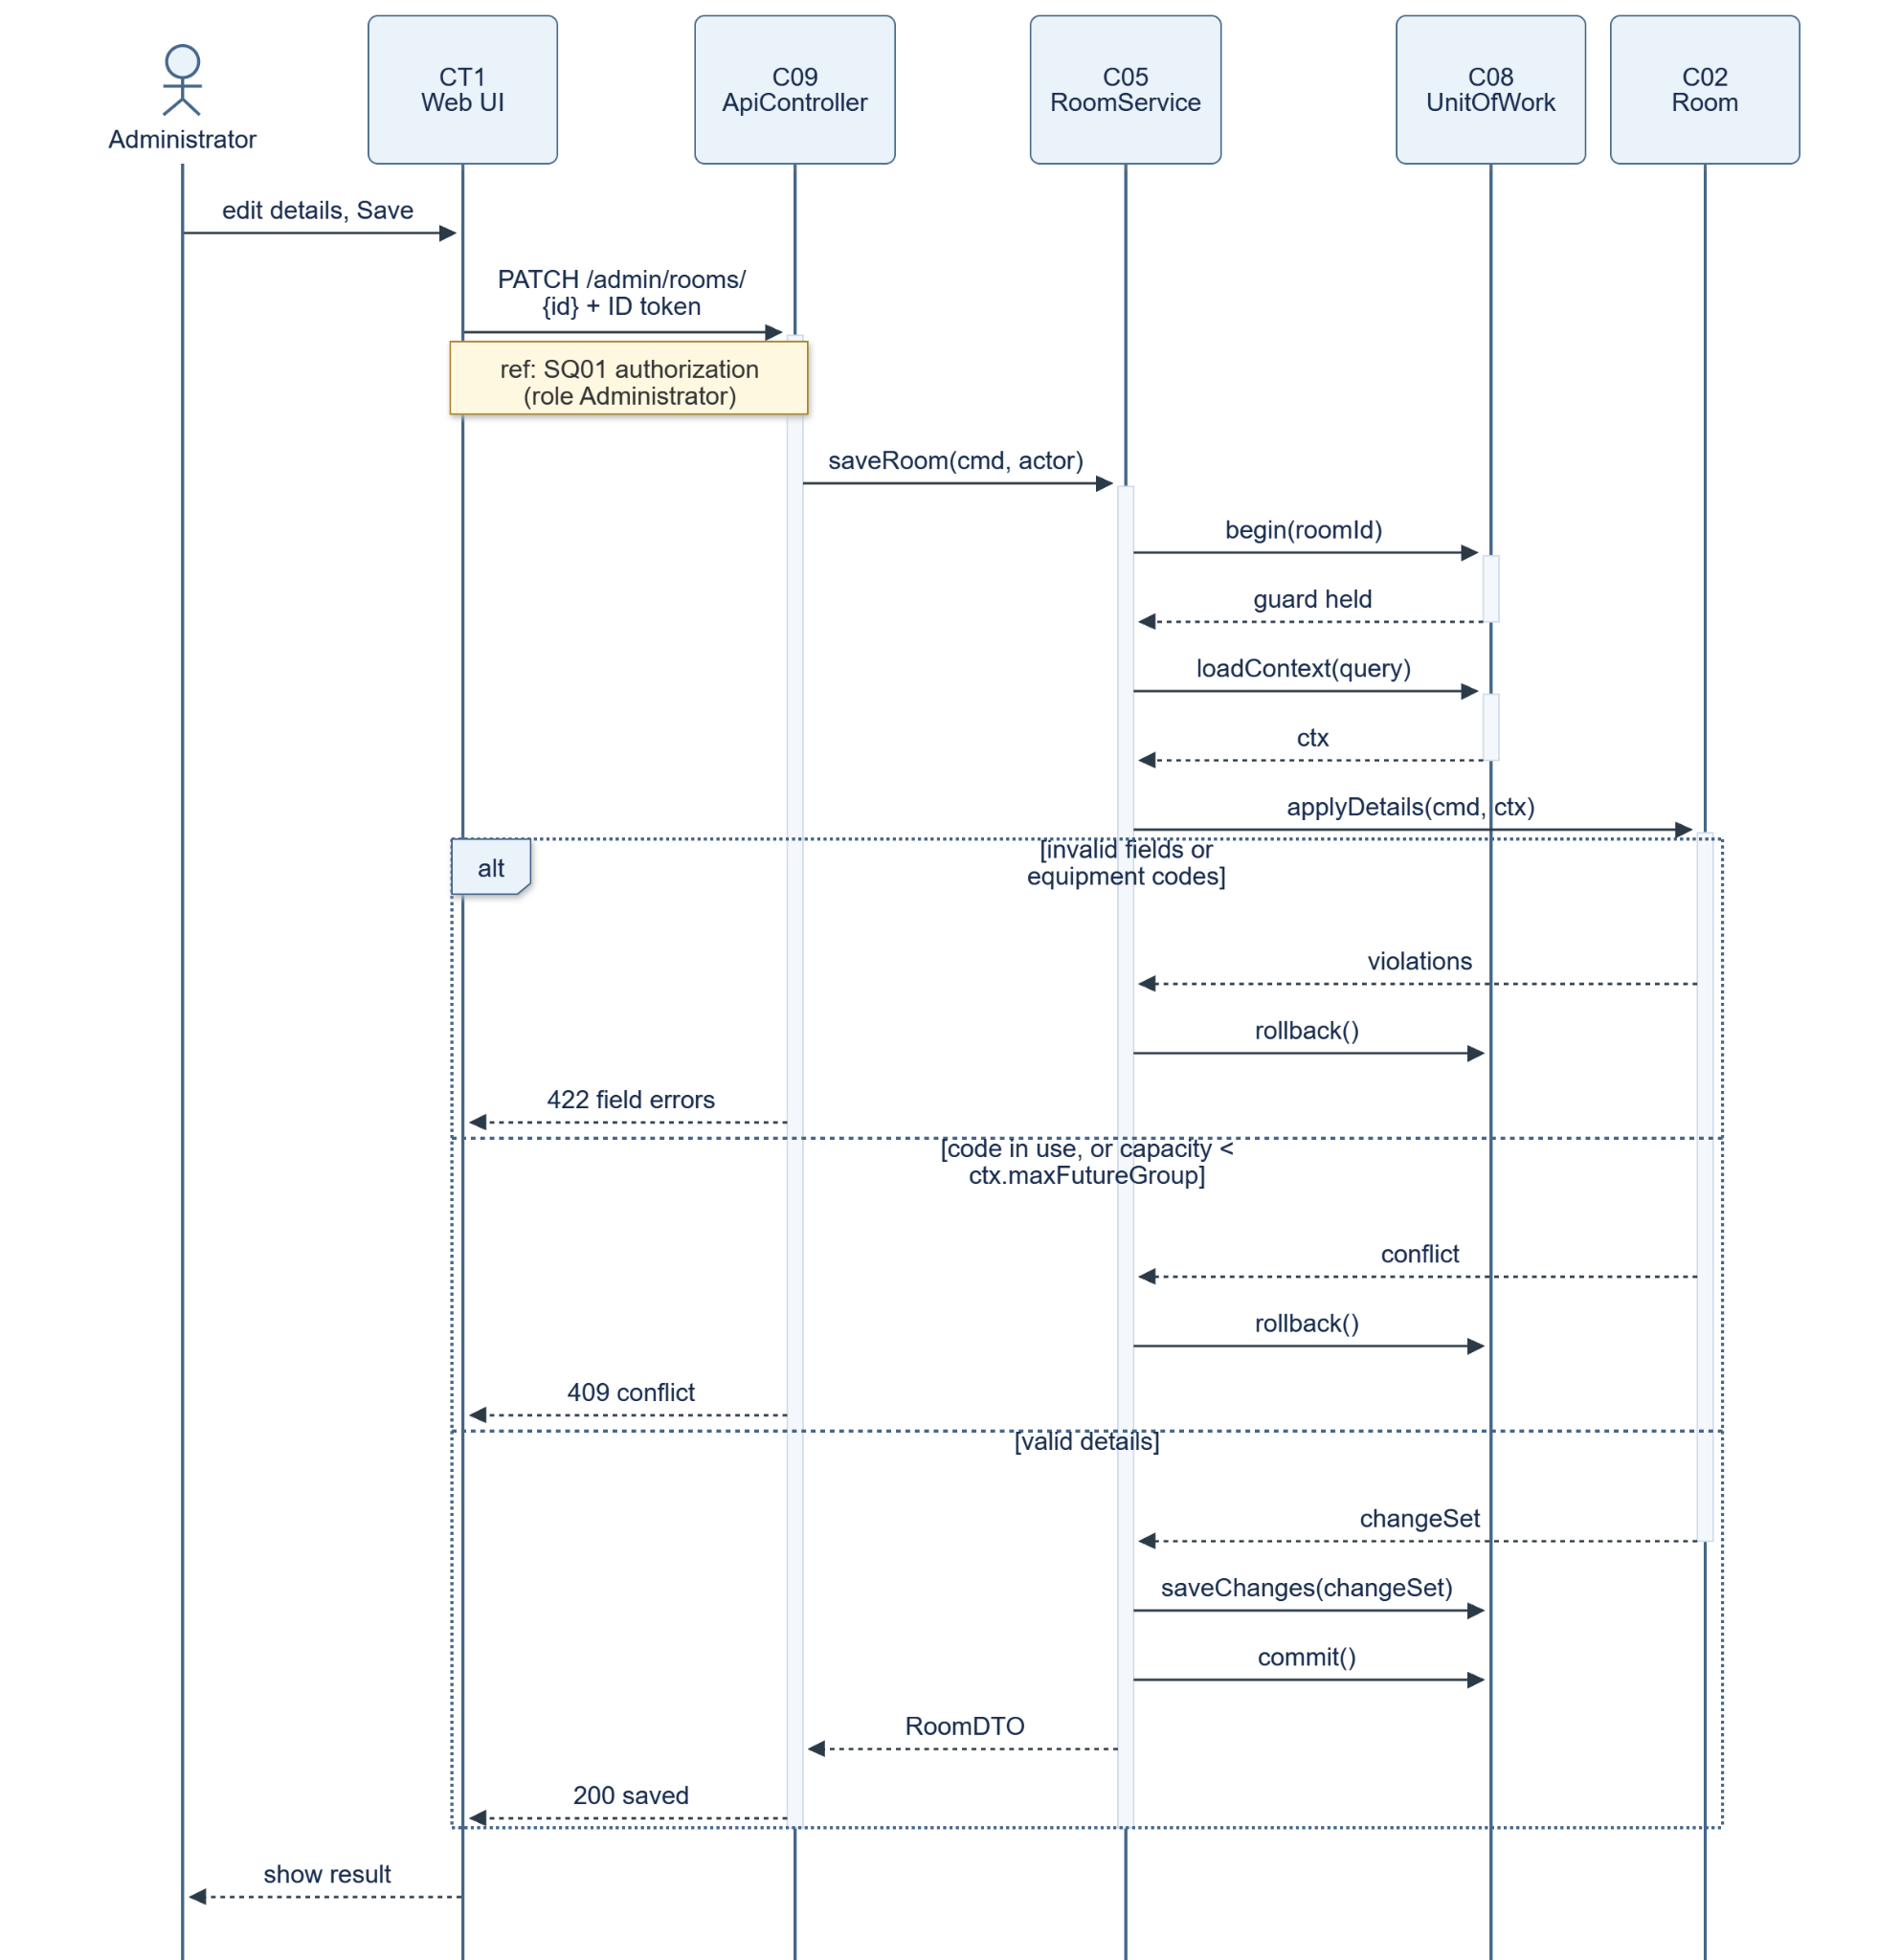
\includegraphics[width=0.94\textwidth,height=0.60\textheight,keepaspectratio]{images/05-object-oriented-design/figure_09.png}
\end{center}
\roomfourfigurecaption{SQ04}{UC-11 save-time room edit, including the capacity check against future Approved bookings.}
\par\medskip

query returns the largest group size among the room's future Approved bookings and whether the normalized code belongs to another room. Because approval waits on the same room guard, either ordering preserves invariant I05: an approval that commits first is included in maxFutureGroup, and an edit that commits first is the capacity the approval checks. A concurrent creation of a different room with the same code is not serialized by this guard; the normalized unique index rejects it at saveChanges (23505 → 409). Creating a new room uses begin(null) and C02.create.\par

\subsubsection{SQ05 UC-13 Create maintenance block}

\par\medskip
\begin{center}
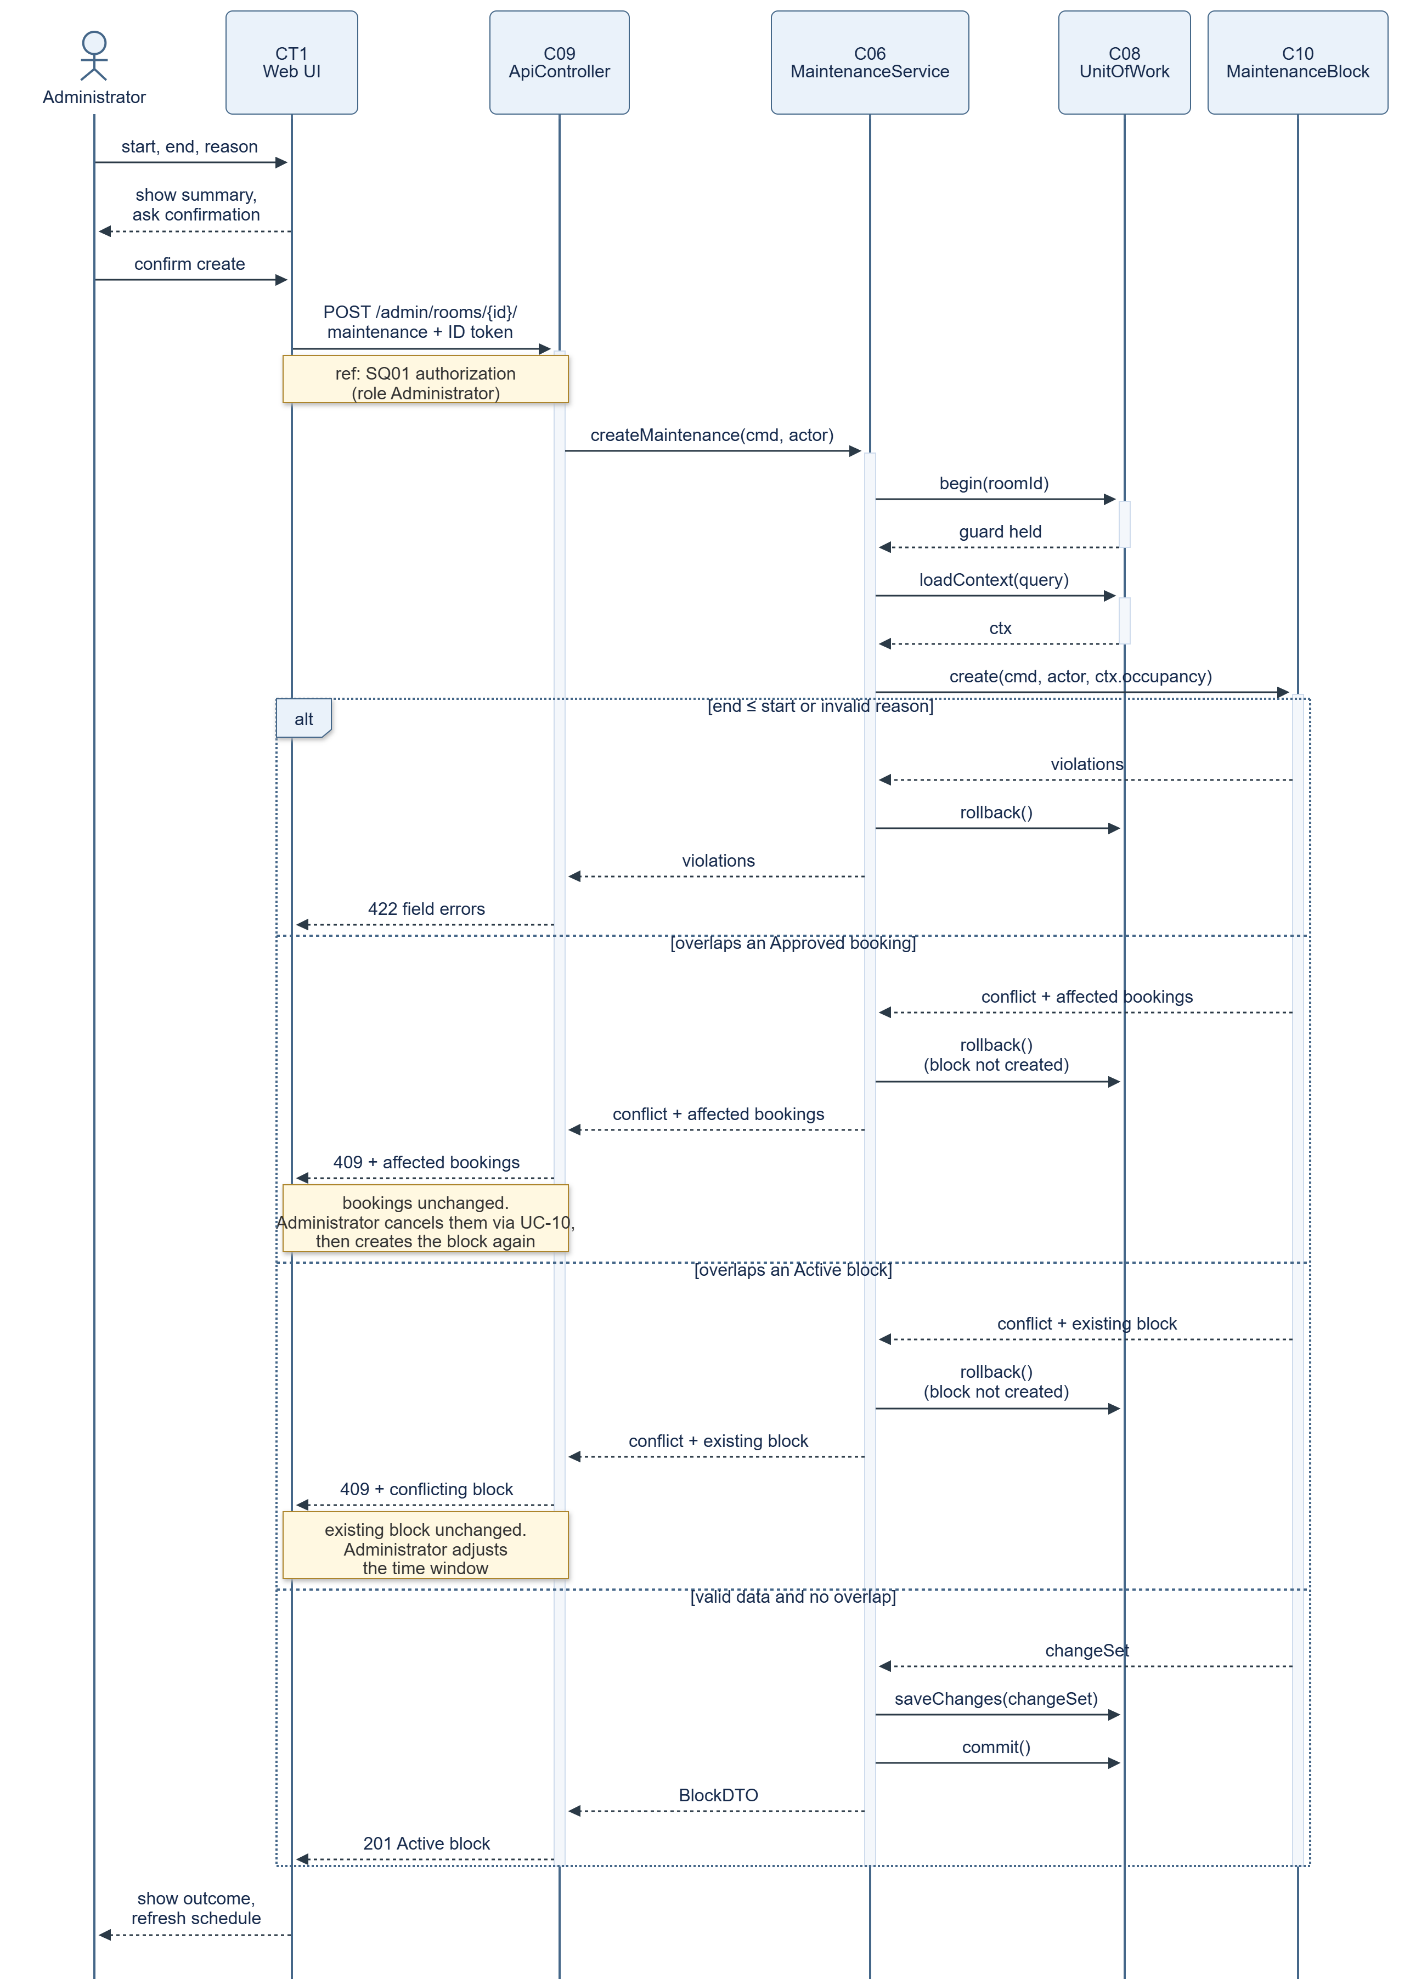
\includegraphics[width=0.94\textwidth,height=0.60\textheight,keepaspectratio]{images/05-object-oriented-design/figure_10.png}
\end{center}
\roomfourfigurecaption{SQ05}{UC-13 maintenance creation without automatic booking cancellation.}
\par\medskip

C10.create validates the window and reason, then checks overlap against Approved bookings and active blocks in ctx.occupancy. Each conflict rolls back and returns HTTP 409 with error.code = SCHEDULE\_CONFLICT, error.requestId and error.conflicts. Following SQ05, if Approved bookings overlap, conflicts lists those bookings first; each item has kind = approved\_booking, bookingRequestId, startAt and endAt. Only when no Approved booking overlaps does conflicts contain the overlapping active maintenance block, with kind = maintenance\_block, maintenanceBlockId, startAt and endAt. S08 can link booking conflicts to UC-10, where the Administrator handles each eligible booking separately before creating the block again; no booking is cancelled automatically (BR-15). A maintenance-block conflict leaves the existing block unchanged so that the Administrator can choose another time window. Removal (UC-13 A1) follows the same frame: roomIdOf(block), begin, loadContext, C10.remove(actor, ctx.now), saveChanges and commit. It marks the block removed with remover and time, deletes only its occupancy row and returns 409 at or after the block start.\par

\subsection{State machine diagrams}

\par\medskip
\begin{center}
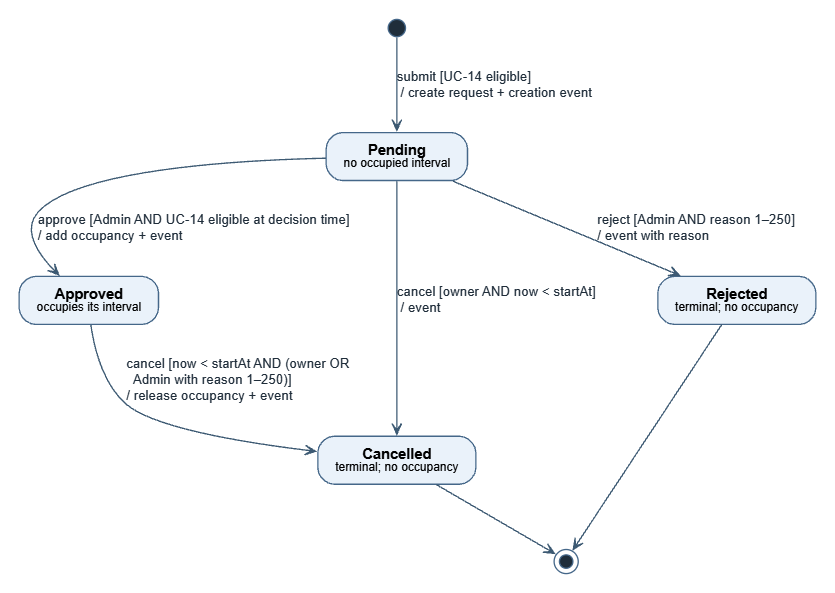
\includegraphics[width=0.94\textwidth,height=0.60\textheight,keepaspectratio]{images/05-object-oriented-design/figure_11.png}
\end{center}
\roomfourfigurecaption{U05}{BookingRequest states. Transitions are written event [guard] / action; Rejected and Cancelled are final.}
\par\medskip

Guards are evaluated at decision time after the room lock, and each successful transition appends exactly one event. The five transitions are the only previous/new status pairs allowed in booking\_events (Section 6). No transition is triggered by time alone: a Pending request whose start has passed stays Pending until an Administrator rejects it, and an Approved booking stays Approved after its interval as history. There is no Expired, Completed, check-in or no-show state. A refused transition leaves the state unchanged and records no event.\par

\par\medskip
\begin{center}
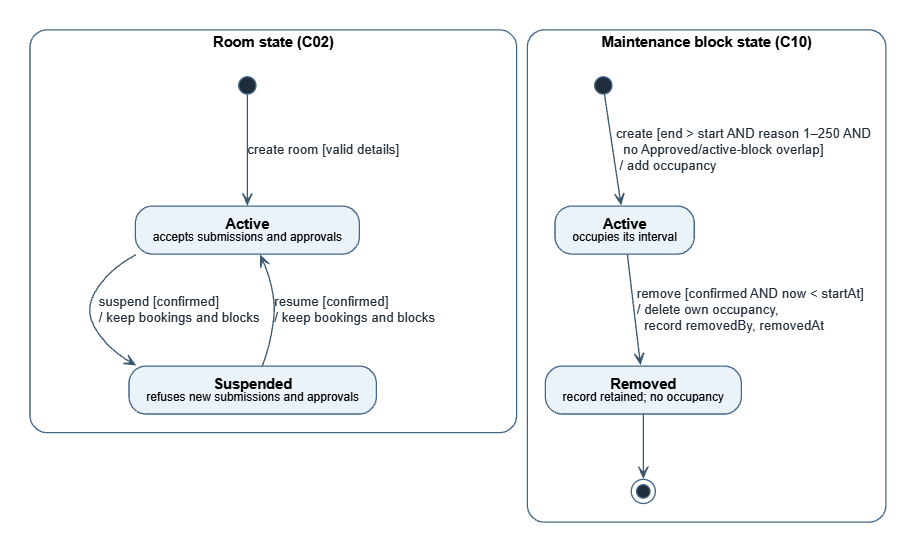
\includegraphics[width=0.94\textwidth,height=0.60\textheight,keepaspectratio]{images/05-object-oriented-design/figure_12.png}
\end{center}
\roomfourfigurecaption{U06}{Independent room and maintenance block states.}
\par\medskip

Suspending or resuming a room never changes bookings, blocks or occupancy (BR-11). A maintenance block that has passed its end time remains active as history; only removal before its start changes its state. Removed is final and the block record is kept.\par

\subsection{Design principles and patterns}

\small
\setlength{\tabcolsep}{3pt}
\renewcommand{\arraystretch}{1.12}
\begin{longtable}{|p{0.23\textwidth}|p{0.31\textwidth}|p{0.38\textwidth}|}
\hline
\textbf{Principle or pattern} & \textbf{Applied at} & \textbf{Reason and limit} \\ \hline
\endfirsthead \hline
Layering, low coupling & C09 → C04–C07, C14 → C01–C03, C10 → C08 & Domain classes import no Express, pg or Firebase code, so rules stay testable. Costs extra interfaces. \\ \hline
Single responsibility, high cohesion & C03 decides eligibility; C04–C06 orchestrate; C08 persists; C14 reads & Each class has one reason to change; avoids a booking "god class". \\ \hline
Information expert, guarded transitions & C01, C02, C10 & Entities own their legal transitions; there is no generic status PATCH. Not the GoF State pattern: four states and one owner make guarded methods simpler (KISS, YAGNI). \\ \hline
Dependency inversion & uowFactory, policy and clock in services; AccountRepository and ReadRepository interfaces & PA4 unit tests can use fakes and a fixed clock for boundaries (08:00, 20:00, now + 7 days) without Firebase or a database. \\ \hline
Unit of Work and Repository & C08 & One client per command: request, occupancy and events commit or roll back together (I01–I06). All writers must use it. \\ \hline
Factory method & Static create on C01, C02, C10; uowFactory & Initial state and creation event are set in one place. \\ \hline
Adapter & C12 & Isolates the Firebase Admin SDK; changing the identity provider affects one class. \\ \hline
Facade & C08 & Hides the pg client, SQL and constraint-error mapping behind seven operations. \\ \hline
Explicit DTO projection & C14 and response DTOs & Privacy follows the returned fields as well as route checks (BR-16, I08). \\ \hline
Idempotent command & C04.submit, C01.matchesSubmission & One logical submission produces one request and one event, even after a lost response (ADR-004). \\ \hline
DRY & TimeInterval.overlaps & One implementation of BR-06 is shared by booking eligibility and maintenance conflicts. \\ \hline
\end{longtable}
\normalsize

% !TEX root = ../\allowbreak{}main.tex

% Section 6 — Data Design

\section{Data Design}

\subsection{Data diagram}

\begin{center}

\includegraphics[width=\textwidth,height=0.72\textheight,keepaspectratio]{images/06-data-design-assets/data-design-image-1.png}

\emph{\textbf{Figure 6.1.} Room4U data design diagram.}

\end{center}

DB01 presents the physical data model of Room4U. Seven tables store pre-created user accounts and profile data, room details, individual room-equipment selections, booking requests, booking events, maintenance blocks and the shared occupancy projection. Each room may have zero or more room\allowbreak\_\allowbreak{}equipment rows, and each row belongs to exactly one room. Its composite primary key prevents duplicate selections for the same room. Each room\allowbreak\_\allowbreak{}occupancy row selects exactly one source: either a booking request or a maintenance block. Each Approved request has one matching occupancy row; Pending, Rejected and Cancelled requests have none. Each active maintenance block has one matching occupancy row, while a removed block has none.\par

Composite foreign keys require the selected source, room and interval to match. The exclusion constraint prevents overlapping occupancy intervals for the same room. Correspondence between source status and occupancy, and the creation of booking events, is enforced by the shared command transaction defined in Section 4.6.\par

Each booking event belongs to one request and one actor. Successful request creation records an initial event, and each successful status transition appends another event in the same transaction. Normal application operations do not hard-delete users, rooms, requests, booking events or maintenance source records. Occupancy rows may be deleted when the corresponding booking is cancelled or maintenance block is removed.\par

\subsection{Data specifications}

\subsubsection{Users}

\begin{longtable}{|p{0.140\textwidth}|p{0.160\textwidth}|p{0.240\textwidth}|p{0.320\textwidth}|}

\hline

\textbf{Column} & \textbf{Data type} & \textbf{Constraints} & \textbf{Description} \\ \hline

\endfirsthead

\hline

\textbf{Column} & \textbf{Data type} & \textbf{Constraints} & \textbf{Description} \\ \hline

\endhead

id & uuid & PK; NOT NULL & Internal account ID generated by the application. \\ \hline

firebase\allowbreak\_\allowbreak{}uid & varchar(128) & UNIQUE; NOT NULL & Verified Firebase identity reference used for account lookup. \\ \hline

email & text & NOT NULL & Provisioned account email displayed in authorized account and request views. \\ \hline

full\allowbreak\_\allowbreak{}name & text & NOT NULL; non-empty after trimming & Provisioned display name for the account bar, requester details and actor displays. \\ \hline

student\allowbreak\_\allowbreak{}code & text & NULL allowed; no new fixed-length or uniqueness rule introduced & Provisioned Student identifier; may be NULL for Administrator accounts. \\ \hline

phone & text & NULL allowed & Provisioned contact value; stored as text to preserve leading zeroes and optional international prefixes. \\ \hline

role & text & NOT NULL; CHECK Student/\allowbreak{}Administrator & Server-owned application role. \\ \hline

created\allowbreak\_\allowbreak{}at & timestamptz & NOT NULL & Account provisioning time. \\ \hline

\end{longtable}

\vspace{2mm}

Profile values are provisioned with the pre-created accounts. Student seeds supply the displayed student identifier; Administrator accounts may have no student\allowbreak\_\allowbreak{}code. Missing optional values are displayed consistently as unavailable information. Room4U adds no public registration or profile-editing workflow. Firebase handles passwords; users stores no password or full identity token. Request ownership and event actors are derived from the authenticated account, not from profile fields submitted by the browser. Requester profiles are returned only in owner- or Administrator-authorized detail views, never in shared room calendars.\par

\subsubsection{rooms}

\begin{longtable}{|p{0.140\textwidth}|p{0.160\textwidth}|p{0.240\textwidth}|p{0.320\textwidth}|}

\hline

\textbf{Column} & \textbf{Data type} & \textbf{Constraints} & \textbf{Description} \\ \hline

\endfirsthead

\hline

\textbf{Column} & \textbf{Data type} & \textbf{Constraints} & \textbf{Description} \\ \hline

\endhead

id & uuid & PK; NOT NULL & Stable room identity. \\ \hline

code & text & NOT NULL; non-empty after trimming; normalized unique index & Trimmed, case-insensitive room-code uniqueness. \\ \hline

name & varchar(80) & NOT NULL; trimmed length 1–80 & Room display name. \\ \hline

floor & text & NULL allowed; no fixed floor enumeration introduced & Floor information used by room details and floor filters. \\ \hline

capacity & integer & NOT NULL; CHECK 1–50 & Current capacity; reductions are checked against future Approved bookings inside the shared room guard. \\ \hline

description & varchar(250) & NULL allowed; maximum 250 characters & Optional room description from the PA2 S07 specification. \\ \hline

photo\allowbreak\_\allowbreak{}ref & text & NULL allowed & Preloaded image reference; missing values use a placeholder. \\ \hline

state & text & NOT NULL; CHECK active/\allowbreak{}suspended & Controls new submissions and approvals. \\ \hline

created\allowbreak\_\allowbreak{}at /\allowbreak{} updated\allowbreak\_\allowbreak{}at & timestamptz & NOT NULL & Creation and latest room-update metadata. \\ \hline

\end{longtable}

\vspace{2mm}

Equipment selections are stored in room\allowbreak\_\allowbreak{}equipment. Room DTOs return equipmentCodes and an equipmentDescription generated from the shared code-to-label mapping. The generated description remains within the PA2 250-character bound. No independently editable equipment string is stored in rooms. Room details retain floor information but introduce no area or zone field. In the current single-library scope, the library and group-study-room labels may be fixed interface information.\par

Floor nullability is unchanged by ADR-005; UI requiredness follows the agreed S07 specification. Under Maintenance is derived from active maintenance intervals and the time being viewed, rather than added as a third rooms.state value.\par

\subsubsection{room\allowbreak\_\allowbreak{}equipment}

\begin{longtable}{|p{0.140\textwidth}|p{0.160\textwidth}|p{0.240\textwidth}|p{0.320\textwidth}|}

\hline

\textbf{Column} & \textbf{Data type} & \textbf{Constraints} & \textbf{Description} \\ \hline

\endfirsthead

\hline

\textbf{Column} & \textbf{Data type} & \textbf{Constraints} & \textbf{Description} \\ \hline

\endhead

room\allowbreak\_\allowbreak{}id & uuid & FK rooms.id; NOT NULL; composite PK part & Room to which the selected equipment belongs. \\ \hline

equipment\allowbreak\_\allowbreak{}code & text & NOT NULL; composite PK part; CHECK approved equipment codes & One selected equipment capability. \\ \hline

row identity & composite PRIMARY KEY & room\allowbreak\_\allowbreak{}id, equipment\allowbreak\_\allowbreak{}code & Prevents duplicate equipment selections for the same room. \\ \hline

\end{longtable}

\vspace{2mm}

The proposed equipment codes are WHITEBOARD, DISPLAY\allowbreak\_\allowbreak{}SCREEN, POWER\allowbreak\_\allowbreak{}OUTLET, AIR\allowbreak\_\allowbreak{}CONDITIONER and WIFI, with Vietnamese labels defined in ADR-005. Each selected checkbox corresponds to one row. An empty selection is represented by zero rows for the room; the API returns an empty equipmentCodes array. The code catalogue is maintained in the shared design/\allowbreak{}application contract, with matching database checks; this design adds no editable equipment catalogue.\par

Creating or editing a room validates all equipment codes and saves the room details and equipment set in one transaction. Existing-room edits use the room guard in Section 4.6. Failure preserves the previous room details and complete equipment set. Deleting/\allowbreak{}replacing selection rows is permitted during this controlled save operation; this does not delete room or booking history.\par

Selecting multiple equipment filters requires every selected code to be present. The application validates and de-duplicates filter codes before querying. No selected equipment filter adds no equipment predicate. Equipment selection does not change the existing booking-capacity or schedule-conflict rules.\par

\subsubsection{Proposed DDL fragment}

\begingroup
\small
\begin{samepage}
\begin{verbatim}
CREATE TABLE room_equipment (
    room_id uuid NOT NULL REFERENCES rooms(id),
    equipment_code text NOT NULL,
    CONSTRAINT room_equipment_pk
        PRIMARY KEY (room_id, equipment_code),
    CONSTRAINT room_equipment_code_check CHECK (
        equipment_code IN (
            'WHITEBOARD', 'DISPLAY_SCREEN', 'POWER_OUTLET',
            'AIR_CONDITIONER', 'WIFI'
        )
    )
);

CREATE INDEX room_equipment_code_room
    ON room_equipment (equipment_code, room_id);
\end{verbatim}
\end{samepage}
\endgroup

\subsubsection{booking\allowbreak\_\allowbreak{}requests}

\begin{longtable}{|p{0.140\textwidth}|p{0.160\textwidth}|p{0.240\textwidth}|p{0.320\textwidth}|}

\hline

\textbf{Column} & \textbf{Data type} & \textbf{Constraints} & \textbf{Description} \\ \hline

\endfirsthead

\hline

\textbf{Column} & \textbf{Data type} & \textbf{Constraints} & \textbf{Description} \\ \hline

\endhead

id & uuid & PK; NOT NULL & One request ID. \\ \hline

owner\allowbreak\_\allowbreak{}id & uuid & FK users.id; NOT NULL & Student owner from AuthContext. \\ \hline

room\allowbreak\_\allowbreak{}id & uuid & FK rooms.id; NOT NULL & Immutable request room. \\ \hline

start\allowbreak\_\allowbreak{}at /\allowbreak{} end\allowbreak\_\allowbreak{}at & timestamptz & NOT NULL; finite; start < end & UTC instants; end derived from selected duration. \\ \hline

group\allowbreak\_\allowbreak{}size & integer & NOT NULL; CHECK ≥1 & Current room capacity checked at submission and approval. \\ \hline

status & text & NOT NULL; four-state CHECK & Pending, Approved, Rejected, Cancelled. \\ \hline

submission\allowbreak\_\allowbreak{}key & uuid & NOT NULL; UNIQUE(owner\allowbreak\_\allowbreak{}id, submission\allowbreak\_\allowbreak{}key) & Technical replay key for one logical submission. \\ \hline

created\allowbreak\_\allowbreak{}at /\allowbreak{} updated\allowbreak\_\allowbreak{}at & timestamptz & NOT NULL & Created order and latest transition metadata. \\ \hline

source identity key & composite UNIQUE & id, room\allowbreak\_\allowbreak{}id, start\allowbreak\_\allowbreak{}at, end\allowbreak\_\allowbreak{}at & Referenced by occupancy FK to prevent wrong room/\allowbreak{}interval projection. \\ \hline

purpose & text & NOT NULL; CHECK GROUP\allowbreak\_\allowbreak{}STUDY/\allowbreak{}PROJECT\allowbreak\_\allowbreak{}DISCUSSION/\allowbreak{}ASSIGNMENT\allowbreak\_\allowbreak{}WORK /\allowbreak{}ACADEMIC\allowbreak\_\allowbreak{}RESEARCH/\allowbreak{}OTHER & Stable purpose code selected through the required S03 dropdown. Vietnamese display labels are defined in ADR-005. \\ \hline

note & varchar(250) & NULL allowed; maximum 250 characters & Optional booking note; blank input may be normalized to NULL. \\ \hline

\end{longtable}

\vspace{2mm}

The submitted room, interval, group size, purpose code and optional note are retained as request data. The API accepts only purpose codes defined in ADR-005 and rejects missing or unsupported values. OTHER remains a valid selected purpose and does not make the note mandatory. Purpose does not introduce booking priority or a new purpose-based approval condition.\par

Request creation replay compares the canonical original submitted values for the same owner and submission key, including the purpose code and note. Note text is trimmed and an empty value is normalized to NULL before storage and replay comparison. An identical replay returns the existing request without creating another request or creation event; reusing the key with different submitted values is refused.\par

No related-course field is stored or inferred from the note. Students may mention a course in free-form note text, but Room4U does not extract or separately manage that information.\par

\subsubsection{Proposed column definitions}

\begingroup
\small
\begin{samepage}
\begin{verbatim}
purpose text NOT NULL CHECK (
    purpose IN (
        'GROUP_STUDY', 'PROJECT_DISCUSSION', 'ASSIGNMENT_WORK',
        'ACADEMIC_RESEARCH', 'OTHER'
    )
),
note varchar(250)
\end{verbatim}
\end{samepage}
\endgroup

\subsubsection{booking\allowbreak\_\allowbreak{}events}

\begin{longtable}{|p{0.140\textwidth}|p{0.160\textwidth}|p{0.240\textwidth}|p{0.320\textwidth}|}

\hline

\textbf{Column} & \textbf{Data type} & \textbf{Constraints} & \textbf{Description} \\ \hline

\endfirsthead

\hline

\textbf{Column} & \textbf{Data type} & \textbf{Constraints} & \textbf{Description} \\ \hline

\endhead

id & bigint identity & PK & Stable event ordering tie-breaker. \\ \hline

request\allowbreak\_\allowbreak{}id & uuid & FK booking\allowbreak\_\allowbreak{}requests.id; NOT NULL & Retained request association. \\ \hline

actor\allowbreak\_\allowbreak{}id & uuid & FK users.id; NOT NULL & Actual server-derived actor. \\ \hline

occurred\allowbreak\_\allowbreak{}at & timestamptz & NOT NULL & Unambiguous server timestamp. \\ \hline

previous\allowbreak\_\allowbreak{}status & text & Nullable only for creation & Prior state; no previous state at creation. \\ \hline

new\allowbreak\_\allowbreak{}status & text & NOT NULL; transition CHECK & Target state; allowed transition pairs only. \\ \hline

reason & varchar(250) & Nullable; trimmed 1–250 if supplied & Required for rejection/\allowbreak{}admin cancellation by service policy. Append events; do not update earlier ones. \\ \hline

\end{longtable}

\vspace{2mm}

The permitted event transitions are NULL → Pending for creation, Pending → Approved, Pending → Rejected, Pending → Cancelled, and Approved → Cancelled. Rejected and Cancelled have no outgoing status transitions.\par

The command service checks the actor, current request status and applicable time conditions before changing the request. It appends the corresponding event in the same transaction. Rejection and Administrator cancellation require a valid reason under BR-13. Earlier events remain unchanged.\par

\subsubsection{maintenance\allowbreak\_\allowbreak{}blocks}

\begin{longtable}{|p{0.140\textwidth}|p{0.160\textwidth}|p{0.240\textwidth}|p{0.320\textwidth}|}

\hline

\textbf{Column} & \textbf{Data type} & \textbf{Constraints} & \textbf{Description} \\ \hline

\endfirsthead

\hline

\textbf{Column} & \textbf{Data type} & \textbf{Constraints} & \textbf{Description} \\ \hline

\endhead

id & uuid & PK; NOT NULL & Stable retained block ID. \\ \hline

room\allowbreak\_\allowbreak{}id & uuid & FK rooms.id; NOT NULL & Target room. \\ \hline

start\allowbreak\_\allowbreak{}at /\allowbreak{} end\allowbreak\_\allowbreak{}at & timestamptz & NOT NULL; finite; start < end & May span local dates/\allowbreak{}closed hours; booking duration rules do not apply. \\ \hline

reason & varchar(250) & NOT NULL; trimmed length 1–250 & Maintenance reason. \\ \hline

state & text & NOT NULL; CHECK active/\allowbreak{}removed & Removed records remain in this table. \\ \hline

created\allowbreak\_\allowbreak{}by & uuid & FK users.id; NOT NULL & Administrator who created the block, derived from AuthContext. \\ \hline

created\allowbreak\_\allowbreak{}at & timestamptz & NOT NULL & Server-recorded creation time. \\ \hline

removed\allowbreak\_\allowbreak{}by & uuid & FK users.id; NULL while active & Administrator who successfully removed the block. \\ \hline

removed\allowbreak\_\allowbreak{}at & timestamptz & NULL while active & Server-recorded removal time. \\ \hline

source identity key & composite UNIQUE & id, room\allowbreak\_\allowbreak{}id, start\allowbreak\_\allowbreak{}at, end\allowbreak\_\allowbreak{}at & Supports occupancy source FK. \\ \hline

\end{longtable}

\vspace{2mm}

An active block has both removed\allowbreak\_\allowbreak{}by and removed\allowbreak\_\allowbreak{}at set to NULL. A removed block has both fields populated. The removal transaction preserves the source record, records the removal actor and time, and deletes only that block's occupancy row. Removal eligibility is checked using the current block state and server decision time after acquiring the room guard.\par

\subsubsection{room\allowbreak\_\allowbreak{}occupancy}

\begin{longtable}{|p{0.140\textwidth}|p{0.160\textwidth}|p{0.240\textwidth}|p{0.320\textwidth}|}

\hline

\textbf{Column} & \textbf{Data type} & \textbf{Constraints} & \textbf{Description} \\ \hline

\endfirsthead

\hline

\textbf{Column} & \textbf{Data type} & \textbf{Constraints} & \textbf{Description} \\ \hline

\endhead

id & bigint identity & PK & Internal schedule projection row. \\ \hline

room\allowbreak\_\allowbreak{}id & uuid & FK rooms.id; NOT NULL & Common exclusion key. \\ \hline

booking\allowbreak\_\allowbreak{}id & uuid? & UNIQUE; composite FK to booking\allowbreak\_\allowbreak{}requests & Present only for an Approved booking projection. \\ \hline

maintenance\allowbreak\_\allowbreak{}id & uuid? & UNIQUE; composite FK to maintenance\allowbreak\_\allowbreak{}blocks & Present only for an active maintenance projection. \\ \hline

start\allowbreak\_\allowbreak{}at /\allowbreak{} end\allowbreak\_\allowbreak{}at & timestamptz & NOT NULL; finite; start < end & Must match the selected source through a composite FK. \\ \hline

source exclusivity & CHECK & Exactly one of booking\allowbreak\_\allowbreak{}id/\allowbreak{}maintenance\allowbreak\_\allowbreak{}id & Never both and never neither. \\ \hline

no overlap & GiST EXCLUDE & room\allowbreak\_\allowbreak{}id = AND tstzrange(start\allowbreak\_\allowbreak{}at,end\allowbreak\_\allowbreak{}at,'[)') \&\& & Reject same-room overlap across booking and maintenance sources. \\ \hline

\end{longtable}

\vspace{2mm}

\subsection{Normalisation and indexes}

Under the stated functional dependencies, the six source tables are designed in Third Normal Form (3NF). They separate account/\allowbreak{}profile data, room details, room-equipment selections, request facts, individual booking events and maintenance facts. Non-key attributes depend on the candidate keys without a transitive dependency through another non-key attribute. Requests reference their owner and room rather than duplicating mutable profile and room details.\par

room\allowbreak\_\allowbreak{}equipment represents each selected capability as a separate row with the composite primary key (room\allowbreak\_\allowbreak{}id, equipment\allowbreak\_\allowbreak{}code). It introduces no repeated checkbox group or editable comma-separated equipment list in rooms. Vietnamese equipment and purpose labels are defined by the shared application contract rather than duplicated in every stored row. Booking duration is calculated from start\allowbreak\_\allowbreak{}at and end\allowbreak\_\allowbreak{}at instead of stored as an independently editable third value.\par

room\allowbreak\_\allowbreak{}occupancy remains a deliberate denormalised projection. It repeats the source room and interval so that one exclusion constraint can prevent conflicts across Approved bookings and active maintenance blocks. Composite foreign keys prevent source, room and interval mismatches. Command services maintain source status, occupancy and booking events within the same transaction, following Section 4.6.\par

The runtime database role may read and append booking\allowbreak\_\allowbreak{}events but must not update, delete or truncate them. It must not delete retained account, room, request or maintenance source records. Occupancy rows may be deleted through the defined cancellation/\allowbreak{}removal operations. room\allowbreak\_\allowbreak{}equipment rows may be inserted or deleted through a validated room-details save transaction. Schema ownership and migration privileges remain separate from the runtime application role.\par

\begin{longtable}{|p{0.260\textwidth}|p{0.300\textwidth}|p{0.300\textwidth}|}

\hline

\textbf{Index or constraint} & \textbf{Frequent operation} & \textbf{Design rationale} \\ \hline

\endfirsthead

\hline

\textbf{Index or constraint} & \textbf{Frequent operation} & \textbf{Design rationale} \\ \hline

\endhead

rooms\allowbreak\_\allowbreak{}code\allowbreak\_\allowbreak{}normalized\allowbreak\_\allowbreak{}uq & Create/\allowbreak{}edit room code. & lower(btrim(code)) implements case-insensitive trimmed uniqueness. \\ \hline

requests\allowbreak\_\allowbreak{}owner\allowbreak\_\allowbreak{}created & Own request list. & owner\allowbreak\_\allowbreak{}id + created\allowbreak\_\allowbreak{}at DESC + id supports stable history paging. \\ \hline

requests\allowbreak\_\allowbreak{}status\allowbreak\_\allowbreak{}created & Admin default queue/\allowbreak{}filter. & status + created\allowbreak\_\allowbreak{}at + id; filter does not impose approval FIFO. \\ \hline

requests\allowbreak\_\allowbreak{}room\allowbreak\_\allowbreak{}future\allowbreak\_\allowbreak{}approved & Save-time capacity check. & Partial index on room\allowbreak\_\allowbreak{}id/\allowbreak{}start\allowbreak\_\allowbreak{}at where status=Approved. \\ \hline

events\allowbreak\_\allowbreak{}request\allowbreak\_\allowbreak{}order & Ordered request history. & request\allowbreak\_\allowbreak{}id + occurred\allowbreak\_\allowbreak{}at + id handles timestamp ties. \\ \hline

maintenance\allowbreak\_\allowbreak{}room\allowbreak\_\allowbreak{}state\allowbreak\_\allowbreak{}start & Admin block list. & Room/\allowbreak{}state/\allowbreak{}start lookup without erasing removed records. \\ \hline

room\allowbreak\_\allowbreak{}occupancy exclusion index & Calendar and overlap check. & GiST room equality plus half-open timestamp-range overlap. \\ \hline

owner\allowbreak\_\allowbreak{}id + submission\allowbreak\_\allowbreak{}key unique & Repeated request creation. & One source request per logical submission key. \\ \hline

room\allowbreak\_\allowbreak{}equipment\allowbreak\_\allowbreak{}pk & Read/\allowbreak{}save a room's selected equipment & Composite key on room\allowbreak\_\allowbreak{}id and equipment\allowbreak\_\allowbreak{}code prevents duplicates and supports room-scoped lookup. \\ \hline

room\allowbreak\_\allowbreak{}equipment\allowbreak\_\allowbreak{}code\allowbreak\_\allowbreak{}room & Search rooms by selected equipment & Index on equipment\allowbreak\_\allowbreak{}code and room\allowbreak\_\allowbreak{}id supports matching rooms against equipment-code filters. \\ \hline

\end{longtable}

\vspace{2mm}

The API and database both restrict purpose and equipment codes to the proposed catalogues in ADR-005. The API rejects unsupported codes instead of trusting that browser controls can only produce valid values. Equipment-filter matching is based on stored codes, not substring searches over translated descriptions. Room equipment and capacity updates share the room-details transaction so partial saves are not exposed.\par

Booking submission and approval apply UC-14 using current decision data. The checks include room state and capacity, 30-minute time boundaries, an allowed duration of 30, 60, 90 or 120 minutes, opening hours of 08:00–20:00 on one local date, server now < start\allowbreak\_\allowbreak{}at ≤ server now + 7 days, and schedule conflicts. Local-time checks use Asia/\allowbreak{}Ho\allowbreak\_\allowbreak{}Chi\allowbreak\_\allowbreak{}Minh.\par

Time-dependent eligibility is evaluated when a command is performed rather than stored as a permanent CHECK constraint. Historical rows remain valid after their scheduled start time passes. Maintenance validates its own interval and reason without applying booking-duration, half-hour alignment or same-local-date restrictions.\par

\subsection{Representative database constraint}

\begingroup
\small
\begin{samepage}
\begin{verbatim}
CREATE EXTENSION IF NOT EXISTS btree_gist;

-- Inside room_occupancy.
EXCLUDE USING gist (
    room_id WITH =,
    tstzrange(start_at, end_at, '[)') WITH &&
);
\end{verbatim}
\end{samepage}
\endgroup

This section presents representative PostgreSQL constraints for the proposed schema. The migration owner must verify extension availability, constraints, service-role privileges and rollback behavior on the chosen PostgreSQL version before implementation acceptance.\par

% Section-local compatibility helpers; packages are loaded by main.tex.
\providecommand{\tightlist}{%
  \setlength{\itemsep}{0pt}\setlength{\parskip}{0pt}}
\providecommand{\maxwidth}{\linewidth}
\providecommand{\maxheight}{\textheight}



\section{User Interface and User Experience Design}\label{user-interface-and-user-experience-design}

This section describes the proposed user interface and user experience
design of Room4U. It defines the screen structure, navigation flows,
detailed screen specifications, control behaviors, validation rules,
event handling, error feedback, responsive layout, and accessibility
considerations.

The design follows the eight screen identifiers (S01--S08) and the
Student and Administrator interfaces established in PA2. The PA2 mockups
are reused as the visual basis for the corresponding PA3 screens. The
control specifications below clarify how the proposed interface should
behave during implementation and verification.

\subsection{Screen List and Flow}\label{screen-list-and-flow}

\subsubsection{7.1.1. Screen List}\label{screen-list}

Room4U provides two role-based interfaces. The Student Interface
supports room discovery, booking requests, request tracking, and
history. The Administrator Interface supports request processing, room
management, and maintenance management.

\small
\setlength{\tabcolsep}{3pt}
\renewcommand{\arraystretch}{1.15}
\begin{longtable}[]{@{}
  >{\raggedright\arraybackslash}p{0.10\textwidth}
  >{\raggedright\arraybackslash}p{0.205\textwidth}
  >{\raggedright\arraybackslash}p{0.16\textwidth}
  >{\raggedright\arraybackslash}p{0.455\textwidth}@{}}
\hline
\begin{minipage}[b]{\linewidth}\raggedright
\textbf{ID}
\end{minipage} & \begin{minipage}[b]{\linewidth}\raggedright
\textbf{Screen Name}
\end{minipage} & \begin{minipage}[b]{\linewidth}\raggedright
\textbf{Use Cases}
\end{minipage} & \begin{minipage}[b]{\linewidth}\raggedright
\textbf{Purpose}
\end{minipage} \\
\hline
\endhead
\hline
\endlastfoot
\textbf{S01} & Sign In & UC-01 & Entry point for Student and
Administrator authentication using provided accounts. \\
\textbf{S02} & Room Search and Availability & UC-02, UC-03 & Search for
suitable rooms and inspect their schedules before requesting a
booking. \\
\textbf{S03} & Booking Request & UC-04 & Submit a booking request for a
selected room using date, start time, duration, group size, purpose, and
optional note. \\
\textbf{S04} & My Requests and History & UC-02, UC-05, UC-06 & Monitor
submitted requests, inspect request details, cancel eligible requests,
and review processed requests. \\
\textbf{S05} & Admin Request Queue & UC-02, UC-07 & Review, search, and
filter student booking requests. \\
\textbf{S06} & Booking Request Details and Processing & UC-07, UC-08,
UC-09, UC-10 & Inspect request details and process Pending or Approved
requests when permitted. \\
\textbf{S07} & Room Management & UC-11, UC-12 & Add and update room
records and suspend or resume rooms. \\
\textbf{S08} & Room Availability and Maintenance & UC-13 & Inspect room
usage and manage maintenance schedules. \\
\end{longtable}
\normalsize

\subsubsection{7.1.2. Navigation Flow}\label{navigation-flow}

\textbf{Student Navigation Flow}

\begin{enumerate}
\def\labelenumi{\arabic{enumi}.}
\item
  Students open S01 and sign in using an account provided by the system.
\item
  After successful authentication, the application verifies the
  user's role and opens S02 for a Student.
\item
  Students search for rooms using the intended date, number of people,
  and room requirements. They can inspect room details and availability.
\item
  After selecting a room and a suitable time slot, students open S03 to
  complete the booking request.
\item
  After a booking request is submitted, the system returns the
  request's actual status and request ID. S04 displays
  the returned request information; the interface must not assume that
  every submission is Pending.
\item
  Students can open S04 directly from the Student navigation menu at any
  time, including before submitting a new request. From S04, they can
  monitor their requests, inspect full request details, cancel an
  eligible request, and review previously processed requests in History.
\item
  Students can open S02 from the Student navigation menu to search for
  rooms, open S03 from a selected room and time slot to submit a booking
  request, or open S04 directly from the menu. They can use Log Out to
  return to S01.
\end{enumerate}

\textbf{Administrator Navigation Flow}

\begin{enumerate}
\def\labelenumi{\arabic{enumi}.}
\item
  Administrators open S01 and sign in using an account provided by the
  system.
\item
  After successful authentication, the application verifies the
  user's role and opens the Administrator interface.
  S05, S07, and S08 are each directly accessible from the Administrator
  navigation menu.
\item
  Administrators can open S05 directly from the menu to review the
  request queue and filter requests by Pending, Approved, Rejected, or
  Cancelled status.
\item
  Selecting View Details from S05 opens S06. From S06, the administrator
  can inspect the selected request, perform permitted approval,
  rejection, or cancellation actions, and return to S05.
\item
  Administrators can open S07 directly from the navigation menu to add
  rooms, edit room information, and suspend or resume rooms.
\item
  Administrators can open S08 directly from the navigation menu to
  inspect room usage, view maintenance schedules, create maintenance
  blocks, and remove eligible future maintenance blocks.
\end{enumerate}

\textbf{Common Navigation and Session Handling}

The Sign In screen is shared by both roles. The application must verify
authentication and the assigned role before opening protected screens.
Student users must not access administrator-only screens or actions.
Administrator users must not submit student booking requests.

The Log Out option is available from the navigation area. Selecting it
opens a confirmation dialog with Cancel and Log Out actions. Cancel
closes the dialog and keeps the user on the current screen. Log Out ends
the session and returns the user to S01. The PA3 design additionally
requires clearing private client-side data and preventing browser
navigation from restoring a protected view after sign-out.

\emph{Figure~\ref{fig:role-based-navigation-flow} shows the main role-based navigation paths. S02 leads
to S03 when a student selects a room and time slot; S04 is independently
accessible from the Student menu. S05 and S06 provide queue-to-detail
and return navigation, while S05, S07, and S08 are independently
accessible from the Administrator menu. Screen transitions remain
subject to authentication, authorization, request status, and the
relevant booking or maintenance rules.}

\begingroup
\renewcommand{\thefigure}{7.1.2}
\refstepcounter{figure}
\label{fig:role-based-navigation-flow}
\begin{center}
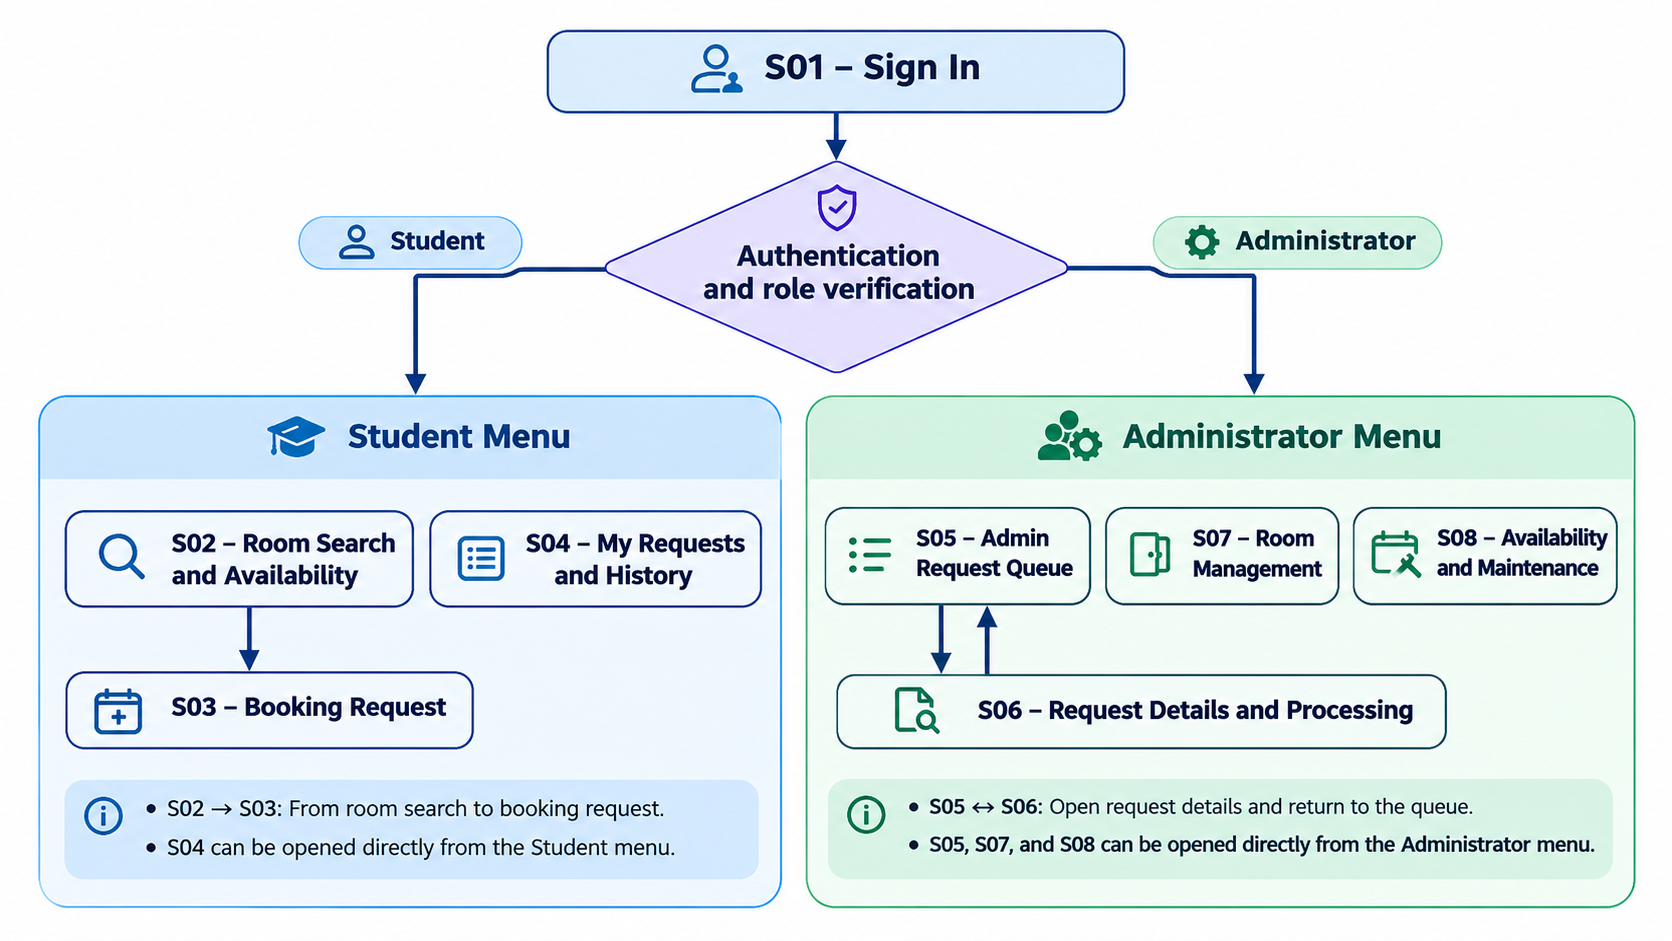
\includegraphics[width=\textwidth,height=0.72\textheight,keepaspectratio]{images/figures/image1.png}
\emph{\textbf{Figure \thefigure.} Proposed role-based navigation flow.}
\end{center}
\endgroup


\subsection{Screen Designs and Detailed
Specifications}\label{screen-designs-and-detailed-specifications}

The following subsections describe the eight screens using the
corresponding mockups from PA2. Detailed control specifications are
provided for S02, S03, S04, S06, S07, and S08. The interface labels
shown in the mockups are Vietnamese, consistent with the Room4U target
users.

\subsubsection{7.2.1. S01 -- Sign In}\label{s01-sign-in}

\textbf{Description:} This screen is the entry point for both Student
and Administrator users. It provides Email and Password fields and a
Sign In button. Users sign in with accounts provided by the system; no
public registration flow is shown. The screen includes Room4U branding
and a short explanation of the service. If authentication fails, an
error message is displayed so the user can check the credentials and try
again.

\textbf{Interaction and Error Handling:} Successful authentication is
followed by application-role verification and navigation to the
appropriate role-based home screen. Failed authentication displays a
generic credential error and allows the user to retry. Registration and
password recovery are outside the PA2 scope.

\begin{center}
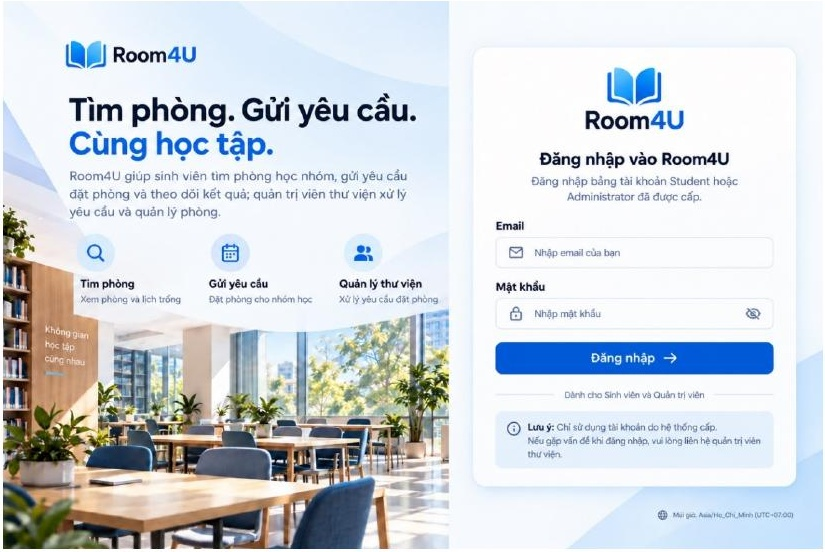
\includegraphics[width=\textwidth,height=0.72\textheight,keepaspectratio]{images/figures/image2.jpg}
\emph{\textbf{Figure 7.2.1.} S01 -- Sign In.}
\end{center}


\subsubsection{7.2.2. S02 -- Room Search and
Availability}\label{s02-room-search-and-availability}

\textbf{Description:} This flow helps students find a suitable meeting
room and check its schedule before submitting a booking request. It
consists of room-search results and a room-availability view.

Room Search: Students can search using the intended date, number of
people, and room requirements. Equipment filters use the equipmentCodes
catalogue defined in ADR-005. Multiple selected equipment codes are
combined using AND logic: a room is returned only when it has every
selected equipment item. Results are presented as room cards showing a
room image, room name, capacity, floor, equipment, current status, and
an action to inspect the room or its availability.

\textbf{Room Availability:} After selecting a room, students can view
its time-slot schedule for a selected date. The schedule distinguishes
available periods from approved bookings, maintenance periods, and other
unavailable periods so that students can choose a valid time before
opening the booking-request form.

\textbf{Control Specifications}

\small
\setlength{\tabcolsep}{3pt}
\renewcommand{\arraystretch}{1.15}
\begin{longtable}[]{@{}
  >{\raggedright\arraybackslash}p{0.15557200000000002\textwidth}
  >{\raggedright\arraybackslash}p{0.15557200000000002\textwidth}
  >{\raggedright\arraybackslash}p{0.317952\textwidth}
  >{\raggedright\arraybackslash}p{0.290904\textwidth}@{}}
\hline
\begin{minipage}[b]{\linewidth}\raggedright
\textbf{Control}
\end{minipage} & \begin{minipage}[b]{\linewidth}\raggedright
\textbf{Type}
\end{minipage} & \begin{minipage}[b]{\linewidth}\raggedright
\textbf{Description and Validation}
\end{minipage} & \begin{minipage}[b]{\linewidth}\raggedright
\textbf{Event Handling}
\end{minipage} \\
\hline
\endhead
\hline
\endlastfoot
\textbf{Date filter} & Date input & Selects the intended booking date;
must be a valid date. & Search refreshes room results and the
availability view for the selected date. \\
\textbf{Number of people} & Number input / filter & Used to filter rooms
by capacity. & Applying the filter updates the displayed room cards. \\
\textbf{Room requirements} & Checkbox filters & Filters rooms by the
selected equipmentCodes from the ADR-005 equipment catalogue. When
multiple codes are selected, AND logic applies: the room must contain
all selected equipment. An empty selection applies no equipment
restriction. & Changing equipment selections refreshes the search
results using the selected equipmentCodes. \\
\textbf{Room card} & Selectable card & Shows room image, name, capacity,
floor, equipment, and current status. & Selecting the card or
availability action opens the room-availability view. \\
\textbf{Availability schedule} & Calendar / time-slot view &
Distinguishes available, approved-booking, maintenance, and other
unavailable periods. & Selecting a valid time proceeds to the
booking-request form. \\
\end{longtable}
\normalsize

\textbf{Event and Error Handling:} If room-search criteria are invalid,
the interface should identify the relevant input. If room or schedule
data cannot be loaded, the system should display an error and allow
retry. A failed schedule load must not be represented as an empty/free
schedule. Pending requests do not reserve room capacity; availability is
determined by the applicable approved-booking and maintenance records.

\begin{center}
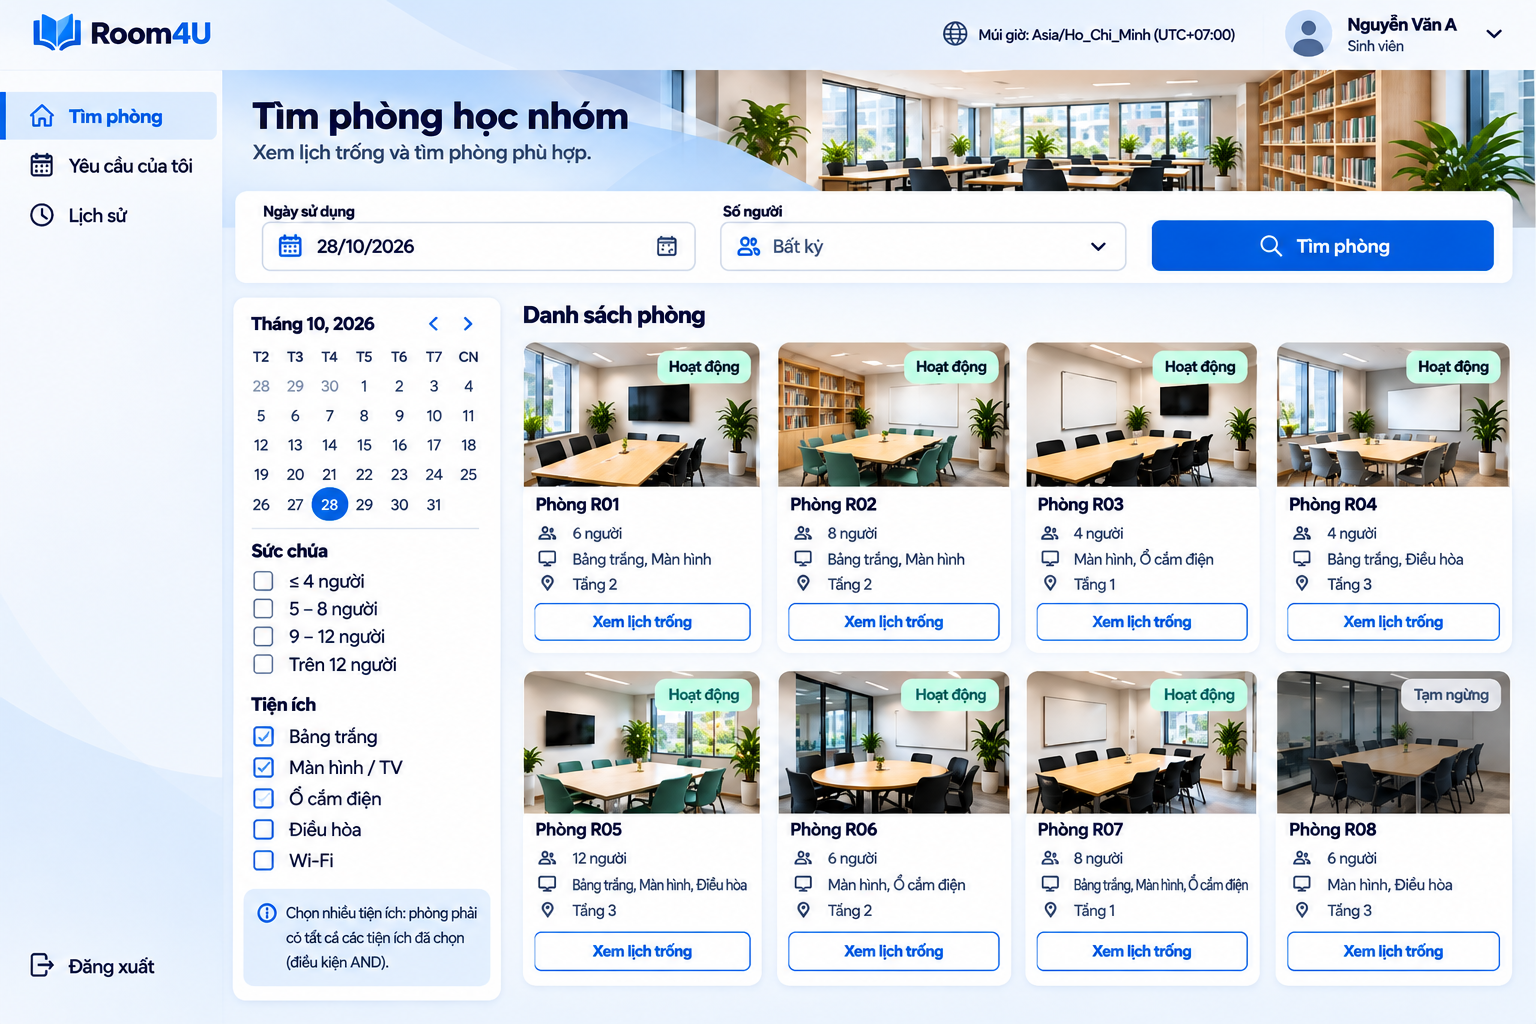
\includegraphics[width=\textwidth,height=0.72\textheight,keepaspectratio]{images/figures/image3.png}
\emph{\textbf{Figure 7.2.2.1.} S02.1 -- Room Search.}
\end{center}


\begin{center}
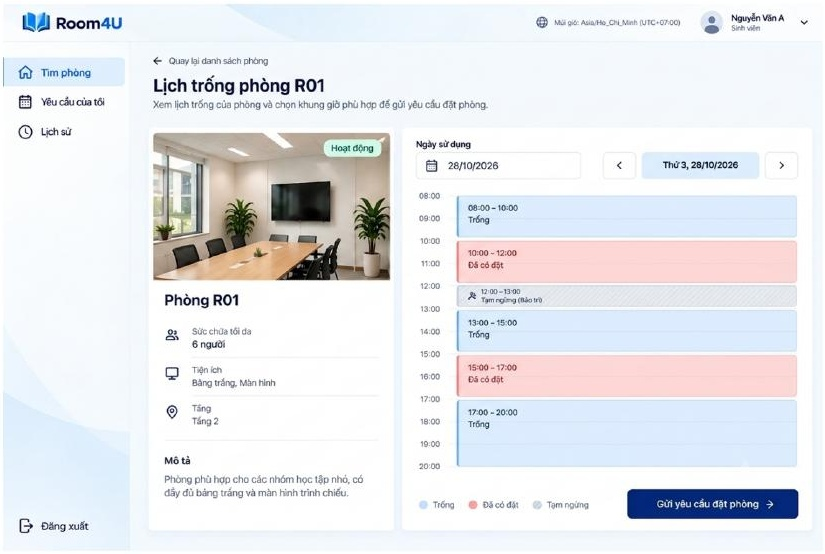
\includegraphics[width=\textwidth,height=0.72\textheight,keepaspectratio]{images/figures/image4.jpg}
\emph{\textbf{Figure 7.2.2.2.} S02.2 -- Room Availability.}
\end{center}


\subsubsection{7.2.3. S03 -- Booking Request}\label{s03-booking-request}

Description: This screen allows a student to submit a booking request
for the selected room. The form displays the room information and
collects the usage date, start time, duration, number of participants,
purpose of use, and an optional note. Purpose of use is a required
dropdown containing only the five purpose codes and Vietnamese labels
defined in ADR-005; arbitrary free text is not accepted. The selected
purpose code is submitted in the purpose API field. The available
duration options are 30, 60, 90, and 120 minutes. Start times must
follow 30-minute increments. The system calculates the end time from the
selected start time and duration. The entire booking must fall within
08:00--20:00 on the same calendar day. The start time must be later than
the current time and no more than seven days from the current time
(BR-04). The participant count must be an integer from 1 through the
selected room's current capacity. The optional note is
limited to 250 characters. The system validates the request against room
capacity, availability, and applicable booking rules.

\textbf{Control Specifications}

\small
\setlength{\tabcolsep}{3pt}
\renewcommand{\arraystretch}{1.15}
\begin{longtable}[]{@{}
  >{\raggedright\arraybackslash}p{0.15557200000000002\textwidth}
  >{\raggedright\arraybackslash}p{0.14885600000000002\textwidth}
  >{\raggedright\arraybackslash}p{0.33147600000000005\textwidth}
  >{\raggedright\arraybackslash}p{0.284096\textwidth}@{}}
\hline
\begin{minipage}[b]{\linewidth}\raggedright
\textbf{Control}
\end{minipage} & \begin{minipage}[b]{\linewidth}\raggedright
\textbf{Type}
\end{minipage} & \begin{minipage}[b]{\linewidth}\raggedright
\textbf{Description and Validation}
\end{minipage} & \begin{minipage}[b]{\linewidth}\raggedright
\textbf{Event Handling}
\end{minipage} \\
\hline
\endhead
\hline
\endlastfoot
\textbf{Selected room} & Read-only summary & Displays selected room
information and current capacity. & Change room returns to S02; no
request is submitted. \\
\textbf{Usage date and start time} & Date/time input & Start time must
be later than the current time, no more than seven days ahead (BR-04),
and aligned to a 30-minute increment. The complete booking interval must
remain within 08:00--20:00 on the same calendar day. & Client-side
validation assists the user; server performs authoritative validation at
submission. \\
\textbf{Duration} & Selection control & Only 30, 60, 90, and 120 minutes
are available. The calculated end time must not exceed 20:00 or cross
into another calendar day. & System calculates and displays the end
time; no independent end-time input is introduced. \\
\textbf{Number of participants} & Number input & Required integer from 1
through the selected room's current capacity. & Invalid
value displays field-level feedback. \\
\textbf{Purpose of use} & Required dropdown & Required selection from
the five values defined in ADR-005. The UI displays the corresponding
Vietnamese label and does not accept arbitrary text. The selected value
is submitted in the purpose API field. & The selected purpose value is
included in the submitted request under the purpose API field. \\
\textbf{Optional note} & Text area & Optional text area; maximum 250
characters. The value is stored in the note field. & The note value is
submitted as note; an empty value means no note was provided. \\
\textbf{Submit / confirmation} & Button and dialog & Student reviews the
booking information before submission. A submissionKey identifies the
logical submission and is retained when retrying the same unchanged
submission after an uncertain response or timeout. & On retry with
unchanged data, the frontend reuses the same submissionKey. If the API
reports that the request already exists, the UI displays that existing
request's actual status and details; it must not create
a duplicate or assume Pending. \\
\end{longtable}
\normalsize

Error Handling and Submission Retry: The system identifies missing or
invalid input and allows the student to correct it. If the room is no
longer available or another booking conflict exists, the request is not
accepted and the interface explains the conflict. A success message is
displayed only after the API confirms the result. If the response is
lost or times out and the outcome is uncertain, retrying the same
unchanged submission must reuse the original submissionKey; a timeout
alone must not cause the frontend to generate a new key. If the API
reports that a request with that key already exists, the interface
displays the existing request and its actual current status returned by
the API. It must not create another request or default the status to
Pending.

\begin{center}
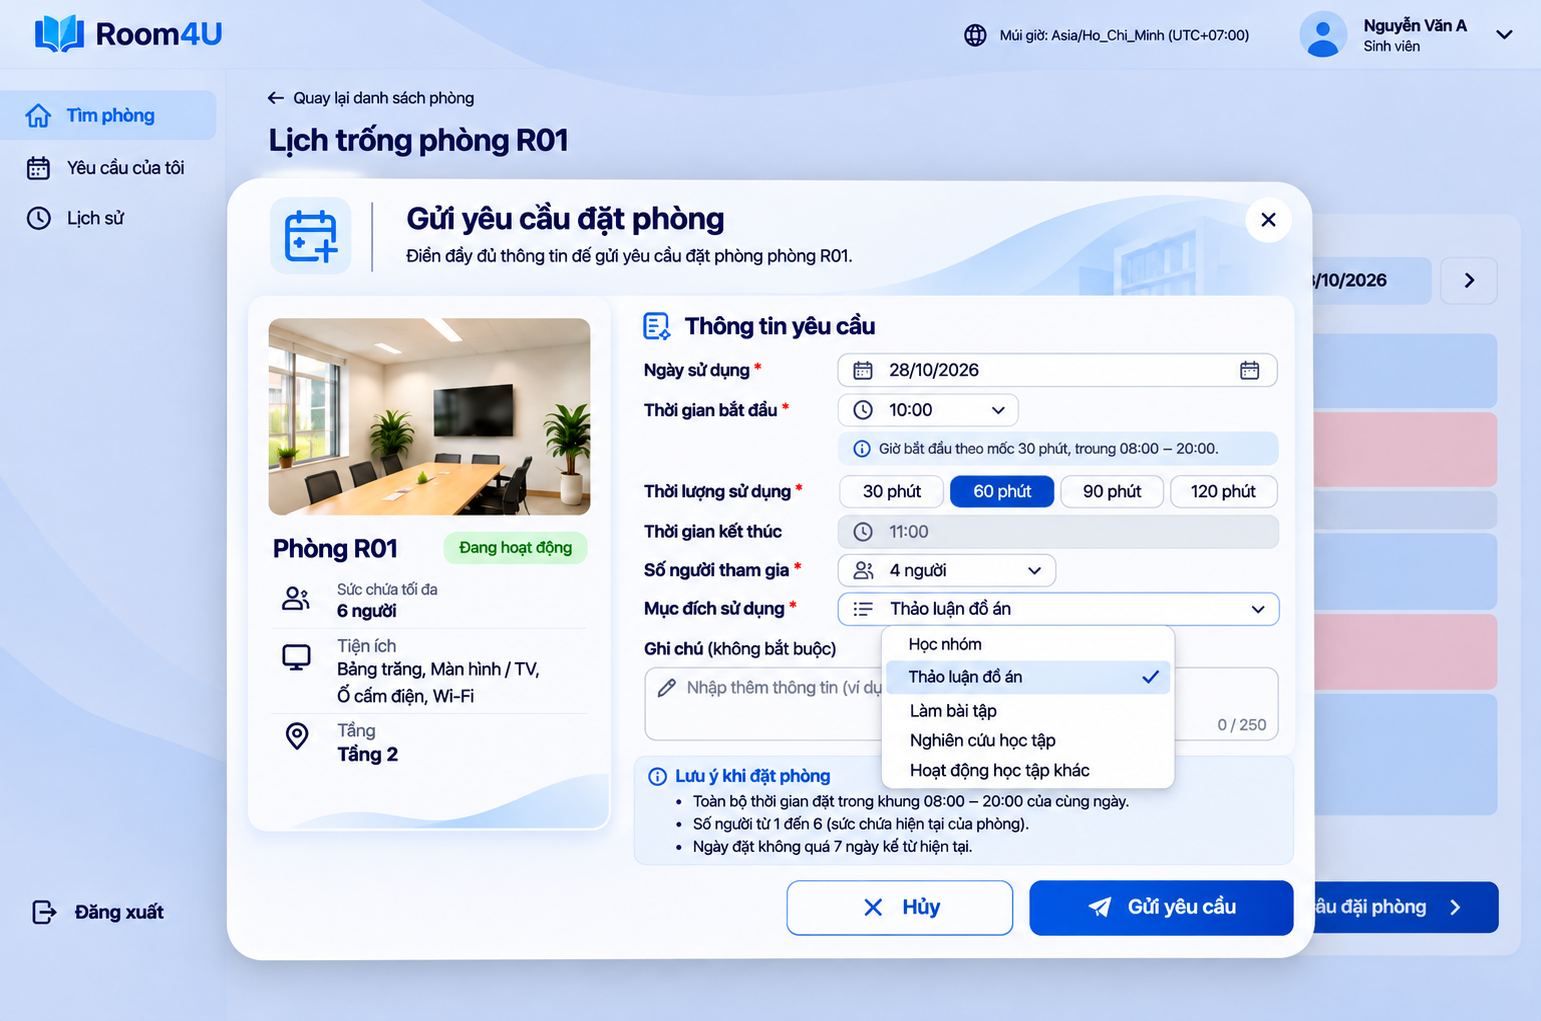
\includegraphics[width=\textwidth,height=0.72\textheight,keepaspectratio]{images/figures/image5.png}
\emph{\textbf{Figure 7.2.3.1.} S03 -- Booking Request form.}
\end{center}


\begin{center}
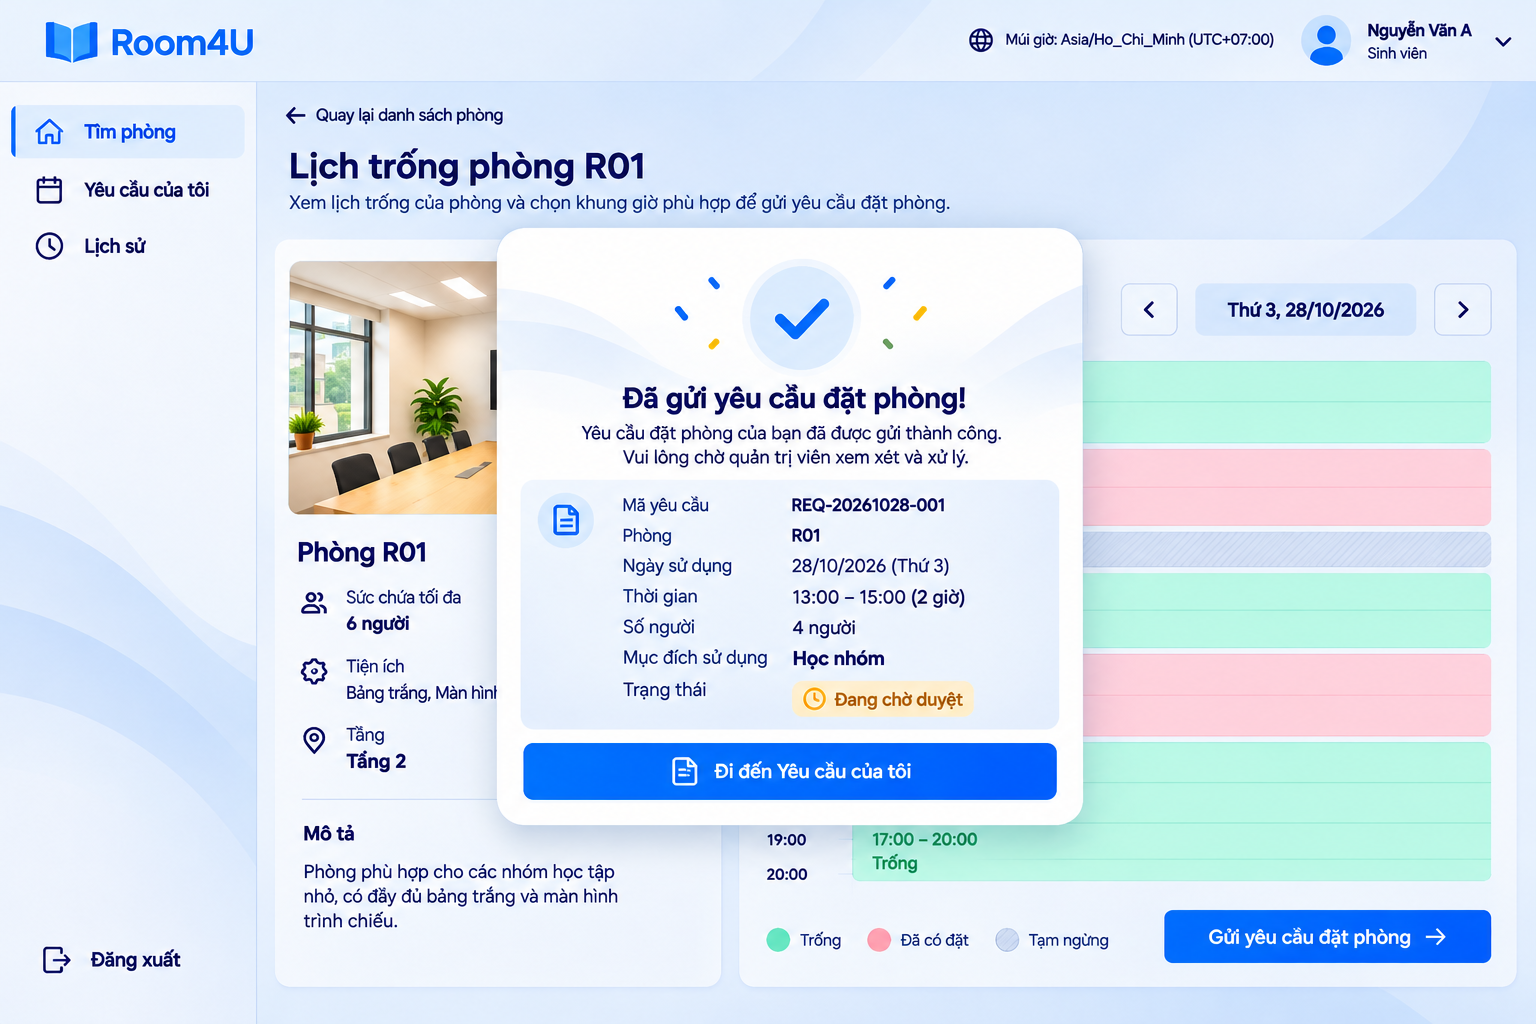
\includegraphics[width=\textwidth,height=0.72\textheight,keepaspectratio]{images/figures/image6.png}
\emph{Figure 7.2.3.2. S03 -- Successful Booking Request Submission.}
\end{center}


\subsubsection{7.2.4. S04 -- My Requests and
History}\label{s04-my-requests-and-history}

\textbf{Description:} This area allows students to monitor submitted
booking requests and review requests that have already been processed.
The active-request screen provides search and status filters. Each row
shows the request ID, room, usage date and time, purpose, current
status, and a View Details action. Students can open a request to
inspect its full information. A separate History screen lists previously
processed requests.

\subsubsection{S04.1 -- My Requests List}\label{s04.1-my-requests-list}

This screen displays the student's request list. Status
tabs help students narrow the results, while the search field supports
searching by request ID, room, or purpose. The table presents the
request ID, room, usage date and time, purpose, status, and a View
Details action. Pagination is provided when the results exceed one page.

\begin{center}
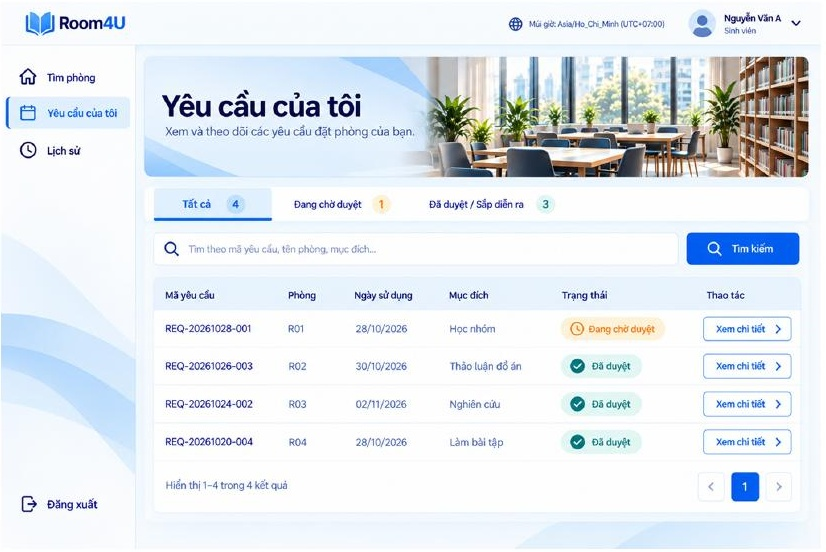
\includegraphics[width=\textwidth,height=0.72\textheight,keepaspectratio]{images/figures/image7.jpg}
\emph{\textbf{Figure 7.2.4.1.} S04.1 -- My Requests List.}
\end{center}


\subsubsection{S04.2 -- Booking Request Details
(Revised)}\label{s04.2-booking-request-details-revised}

This screen presents the full information for one selected request. It
includes the request ID and current status, requester information, room
information, booking information, purpose, and the optional note. The
section labeled ``Mô tả chi tiết yêu
cầu'' displays the content of the note field; it is not
a separate data field.

\begin{itemize}
\item
  \textbf{Requester Information:} Full name, student ID, email address,
  and phone number. These values are supplied from the database.
\item
  \textbf{Room Information:} Room code, room name, building, floor,
  capacity, and equipment. The building information is retained as
  ``Thư viện'' and the floor is retained
  as ``Tầng: 2''. No separate
  room-area/location line is displayed.
\item
  \textbf{Booking Information:} Exactly three evenly arranged
  information cards: ``Thời gian sử dụng'',
  ``Số người đặt'', and
  ``Mục đích sử dụng''.
\item
  Request Description: The purpose is displayed using the Vietnamese
  label mapped from the code stored in the purpose field returned by the
  API. The section labeled ``Mô tả chi tiết yêu
  cầu'' displays the note value. No separate
  detailed-description field exists. Students may mention a course name
  in the optional note; Room4U does not manage enrolled subjects.
\item
  Equipment Information: Equipment labels are resolved from the
  equipment codes returned by the API and displayed using the Vietnamese
  labels in ADR-005.
\item
  \textbf{Request Actions:} Cancel Request is available when the
  applicable request-status and booking-time conditions permit
  cancellation.
\end{itemize}

The ``Môn học liên quan'' field, its book
icon, and its sample value are removed. The ``Vị trí:
Tầng 2, khu A'' line and its location icon are removed.
Room codes such as A-01 and B-01 remain because they are room
identifiers, not area-management data.

\textbf{Control Specifications}

\small
\setlength{\tabcolsep}{3pt}
\renewcommand{\arraystretch}{1.15}
\begin{longtable}[]{@{}
  >{\raggedright\arraybackslash}p{0.15557200000000002\textwidth}
  >{\raggedright\arraybackslash}p{0.14885600000000002\textwidth}
  >{\raggedright\arraybackslash}p{0.33147600000000005\textwidth}
  >{\raggedright\arraybackslash}p{0.284096\textwidth}@{}}
\hline
\begin{minipage}[b]{\linewidth}\raggedright
\textbf{Control}
\end{minipage} & \begin{minipage}[b]{\linewidth}\raggedright
\textbf{Type}
\end{minipage} & \begin{minipage}[b]{\linewidth}\raggedright
\textbf{Description and Validation}
\end{minipage} & \begin{minipage}[b]{\linewidth}\raggedright
\textbf{Event Handling}
\end{minipage} \\
\hline
\endhead
\hline
\endlastfoot
\textbf{Owned request list} & List / compact table & Displays only the
authenticated student's requests and their textual
statuses. & Select opens the corresponding owned request detail; empty
state offers navigation to S02. \\
\textbf{Search} & Text input & Supports request ID, room, or purpose. &
Updates the displayed request list. \\
\textbf{Status filters} & Tabs / selection control & Filters by the
statuses shown in the PA2/PA3 design. & Selecting a status updates the
list without changing request records. \\
\textbf{Request details} & Read-only information & Shows request
ID/status; requester name, student ID, email, phone; room code/name,
building, floor, capacity, equipment; usage period, participant count,
purpose label resolved from the code stored in the purpose API field,
and the note displayed as ``Mô tả chi tiết yêu
cầu''. The note is not a separate field. No subject or
room-area field. & Selecting a request opens details; refresh retrieves
current information. \\
\textbf{Processing history} & Read-only event list & Shows request
events, actor/time, and applicable processing or cancellation reason. &
Refresh retrieves the current request state and history. \\
\textbf{Cancel Request} & Button + confirmation & Only for the
student's own eligible Pending or Approved request
before the scheduled start time. & Confirmation invokes UC-06;
cancel/close leaves the request unchanged. \\
\textbf{Conflict / load feedback} & Status message / retry & Must not
assume cancellation succeeded if the response is lost or uncertain. &
Refresh retrieves the actual request state before displaying the
result. \\
\end{longtable}
\normalsize

\textbf{Cancellation Interaction:} When a student selects Cancel Request
for an eligible request, the system asks for confirmation before
changing the request status. If cancellation is not allowed, the
interface explains why the action cannot proceed. Closing the dialog or
choosing not to continue leaves the request unchanged.

\textbf{History Function:} The History screen allows students to review
previously processed booking requests. It includes Rejected and
Cancelled requests, as well as Approved requests whose scheduled usage
time has passed. An Approved request retains its Approved status; the
interface may indicate that its scheduled time has passed rather than
changing the status to Completed. The history table shows the request
ID, room, usage date, purpose, status, and a View Details action. Search
and pagination help students locate older records.

\textbf{Logout Interaction:} The Log Out option is available in the left
navigation. Selecting it opens a confirmation dialog. Cancel closes the
dialog and keeps the student on the current page; Log Out ends the
session and returns the user to S01.

\begin{center}
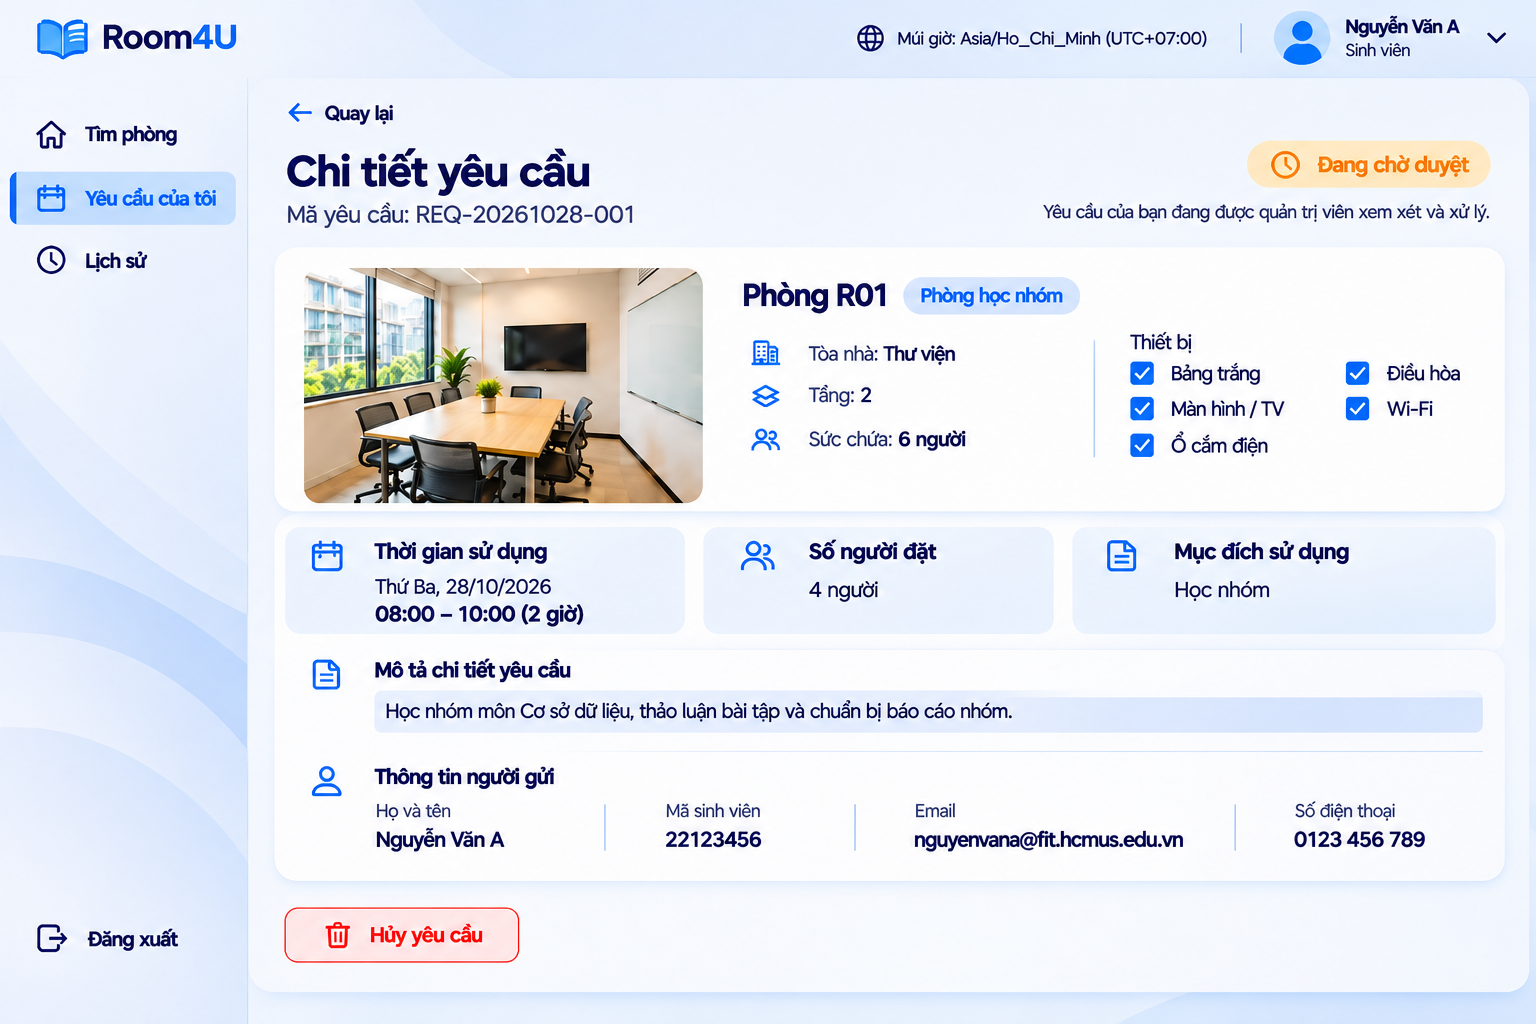
\includegraphics[width=\textwidth,height=0.72\textheight,keepaspectratio]{images/figures/image8.png}
\emph{\textbf{Figure 7.2.4.2.} S04.2 -- Booking Request Details (PA2 mockup
revised to remove subject and room-area fields).}
\end{center}


\begin{center}
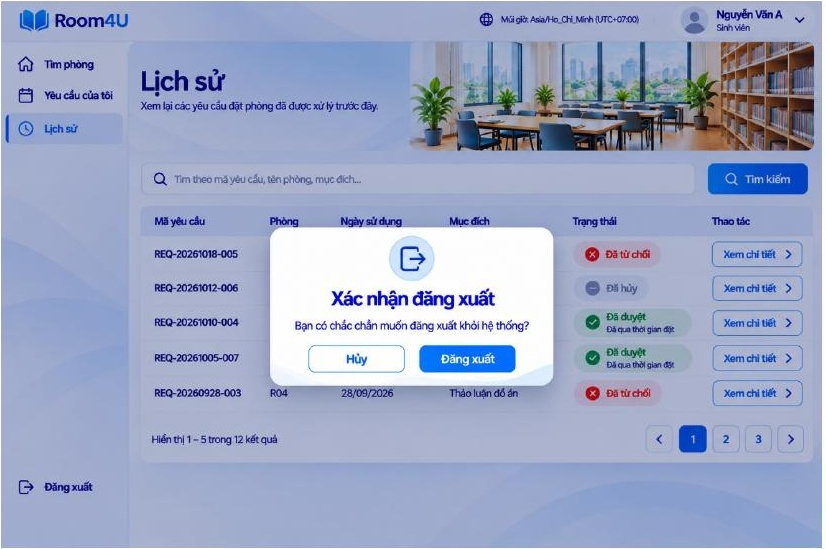
\includegraphics[width=\textwidth,height=0.72\textheight,keepaspectratio]{images/figures/image9.jpg}
\emph{\textbf{Figure 7.2.4.3.} S04 -- History page with Log Out
confirmation.}
\end{center}


\subsubsection{7.2.5. S05 -- Admin Request
Queue}\label{s05-admin-request-queue}

\textbf{Description:} This screen is the administrator's
request-management queue. It provides status categories for Pending,
Approved, Rejected, and Cancelled requests, together with a search field
and a submission-date filter. The request table displays key information
such as request ID, room, requested usage period, number of
participants, submission time, and current status. Administrators select
View Details to inspect and process an individual request.

\textbf{Interaction and Error Handling:} The queue is a read view.
Loading or filtering it does not process a request. Pending is the
default status filter. The Approved filter is required to find bookings
for UC-10. Selecting View Details opens S06. If no request matches the
filters, an empty-state message is displayed; if loading fails, the
administrator can retry.

\begin{center}
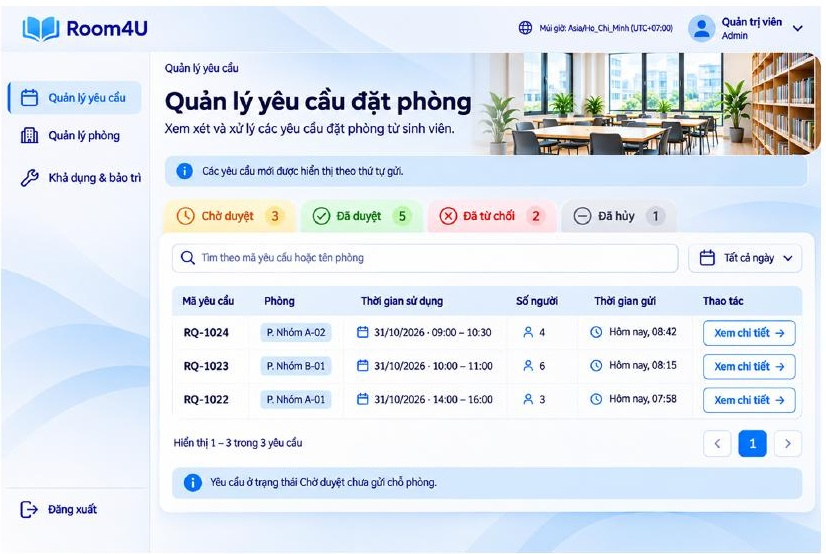
\includegraphics[width=\textwidth,height=0.72\textheight,keepaspectratio]{images/figures/image10.jpg}
\emph{\textbf{Figure 7.2.5.} S05 -- Admin Request Queue.}
\end{center}


\subsubsection{7.2.6. S06 -- Booking Request Details and
Processing}\label{s06-booking-request-details-and-processing}

\textbf{Description:} This screen presents the details and processing
controls for a selected booking request. Its layout changes according to
the request status. Common information includes booking details,
requester information, room information, the room schedule, and
request-processing history.

Pending Requests: Administrators review the requested date and time,
duration, number of participants, purpose, notes, requester details,
room capacity, equipment, and room availability. A Pending request can
be approved only if its scheduled start time has not been reached and
all current scheduling, room, and capacity checks pass. A Pending
request whose start time has arrived or passed must not be approved, but
it may still be rejected by providing a valid rejection reason. Before
approval, the system checks for scheduling conflicts. If the requested
period is no longer available, the interface displays a conflict message
and does not approve the request.

Approved, Rejected, and Cancelled Requests: Administrators can review
the booking information, current status, processing reason when
applicable, and request history. For an Approved request, the Cancel
Booking action is available only before its scheduled start time. The
administrator must enter a valid cancellation reason of 1--250
characters after leading and trailing whitespace are trimmed, and
explicitly confirm the action (BR-13). Rejected and Cancelled requests
are presented for review rather than as pending requests awaiting
approval.

\textbf{Control Specifications}

\small
\setlength{\tabcolsep}{3pt}
\renewcommand{\arraystretch}{1.15}
\begin{longtable}[]{@{}
  >{\raggedright\arraybackslash}p{0.15557200000000002\textwidth}
  >{\raggedright\arraybackslash}p{0.15557200000000002\textwidth}
  >{\raggedright\arraybackslash}p{0.317952\textwidth}
  >{\raggedright\arraybackslash}p{0.290904\textwidth}@{}}
\hline
\begin{minipage}[b]{\linewidth}\raggedright
\textbf{Control}
\end{minipage} & \begin{minipage}[b]{\linewidth}\raggedright
\textbf{Type}
\end{minipage} & \begin{minipage}[b]{\linewidth}\raggedright
\textbf{Description and Validation}
\end{minipage} & \begin{minipage}[b]{\linewidth}\raggedright
\textbf{Event Handling}
\end{minipage} \\
\hline
\endhead
\hline
\endlastfoot
\textbf{Current request details} & Read-only detail & Shows request
status, room/capacity, requester information, booking time, participant
count, and processing history. & Refresh current data before retrying an
action based on stale information. \\
\textbf{Approve} & Button + confirmation & Available only for a Pending
request whose scheduled start time has not been reached. Approval is
subject to current scheduling, room availability, and capacity checks. &
Successful approval updates status; a conflict prevents approval and
displays the cause. \\
\textbf{Reject reason} & Text area + confirmation & Required for
rejection; 1--250 characters after leading and trailing whitespace are
trimmed. A Pending request may still be rejected even when its scheduled
start time has arrived or passed. & Invalid reason is retained with
validation feedback; valid confirmation processes rejection. \\
\textbf{Cancel Booking} & Conditional button + reason & Available only
for an Approved request before its scheduled start time. A valid reason
of 1--250 characters after trimming is required, together with explicit
administrator confirmation (BR-13). & Confirmation processes
cancellation and updates the request to Cancelled. \\
\textbf{Conflict information} & Administrator information panel & Shows
the relevant conflict; does not automatically cancel or modify another
booking. & Administrator reviews the conflict and returns to the request
detail. \\
\end{longtable}
\normalsize

Error Handling: If the request is no longer Pending, approval or
rejection is not performed. A Pending request whose scheduled start time
has arrived or passed cannot be approved, but can still be rejected with
a valid reason. If the requested period conflicts with current
availability, the system displays the conflict and leaves the request
unchanged. For Approved requests, cancellation is allowed only before
the scheduled start time and requires a valid reason and explicit
confirmation. If cancellation is not permitted, the interface explains
why.

\begin{center}
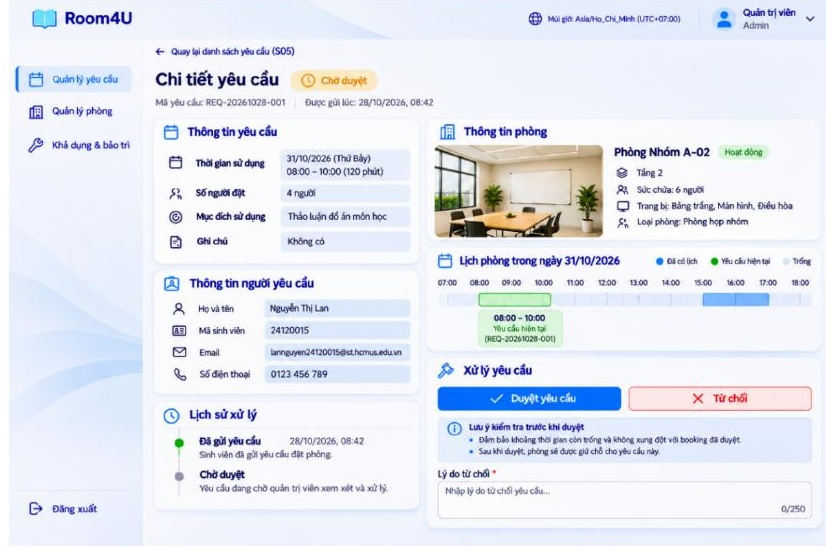
\includegraphics[width=\textwidth,height=0.72\textheight,keepaspectratio]{images/figures/image11.jpg}
\emph{\textbf{Figure 7.2.6.1.} S06.1 -- Pending Request Details.}
\end{center}


\begin{center}
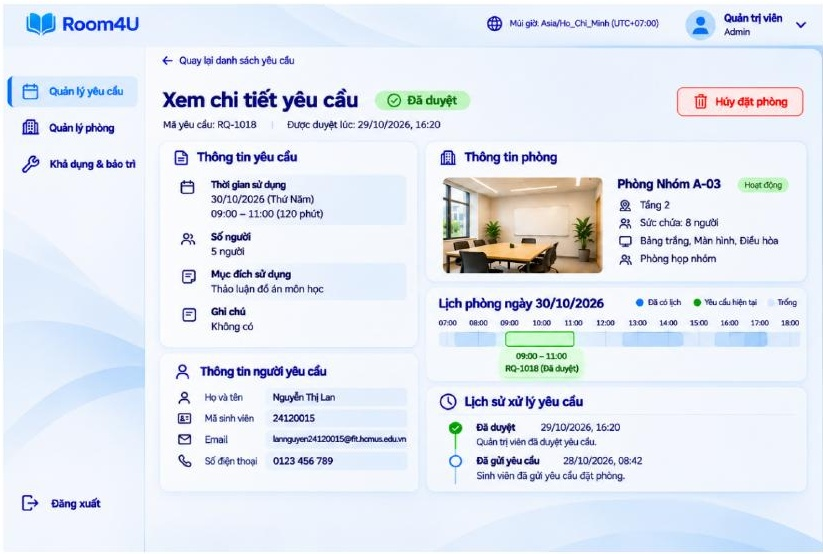
\includegraphics[width=\textwidth,height=0.72\textheight,keepaspectratio]{images/figures/image12.jpg}
\emph{\textbf{Figure 7.2.6.2.} S06.2 -- Approved Request Details and
Cancellation.}
\end{center}


\begin{center}
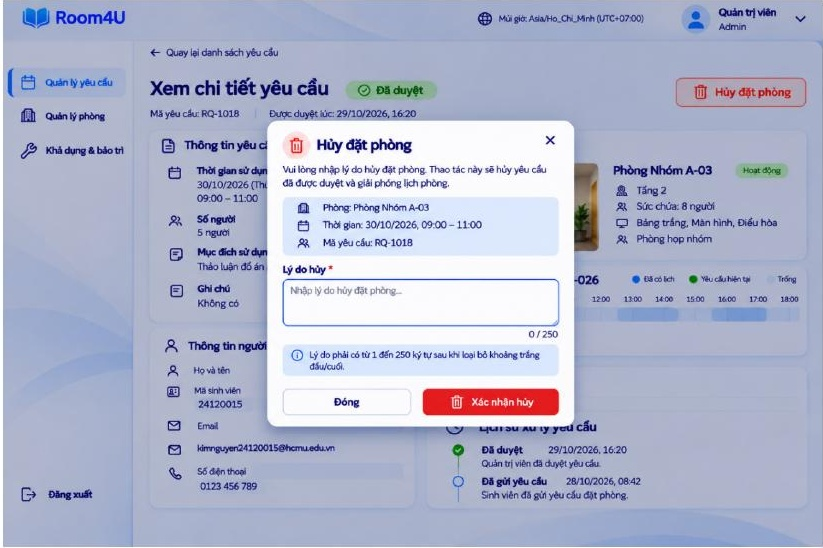
\includegraphics[width=\textwidth,height=0.72\textheight,keepaspectratio]{images/figures/image13.jpg}
\emph{\textbf{Figure 7.2.6.3.} S06.2 -- Approved Booking Cancellation
dialog.}
\end{center}


\subsubsection{7.2.7. S07 -- Room Management}\label{s07-room-management}

\textbf{Description:} This screen allows administrators to manage room
records and monitor each room's current status. It loads the room list
and summary from GET /admin/rooms. Summary cards show the total number of
rooms and mutually exclusive counts of Active, Under Maintenance, and
Suspended rooms. The API classifies every room using one server-selected
asOf: a suspended room is Suspended; an active room with an active
maintenance block satisfying startAt $\leq$ asOf $<$ endAt is Under
Maintenance; every other active room is Active. The same asOf is used
for the list and summary, and the summary always covers all rooms,
regardless of the current list filters. Administrators can search by
room code or name and filter the list by floor or display status. The
room table and detail panel show the room code, room name, floor,
capacity, equipment, description, and display status. After a successful
add, edit, suspend, or resume operation, S07 reloads both the list and
summary.

Room Creation: The Add Room dialog collects a unique room code, room
name, floor, capacity, equipment selections, an optional description, and
an optional selection of an existing room image. The room code must be unique without case sensitivity after
leading and trailing whitespace are removed. The room name is required
and must contain 1--80 characters after trimming leading and trailing
whitespace. Capacity must be an integer from 1 to 50. Equipment
selections come from the complete ADR-005 equipment catalogue, including
``Ổ cắm điện''. The frontend submits
selected equipment as an equipmentCodes array; an empty array means no
equipment is selected. The description is optional and limited to 250
characters. The selected image is submitted as photoRef; when blank, omitted
or null on creation, the default room image is used. After a valid
submission, a success dialog confirms that the new room has been added
and shows its key details.

Room Editing: The Edit Room dialog displays the selected
room's existing information for update. Administrators
can update the room code, name, floor, capacity, equipment, optional
description, and optional selection of an existing room image. The room name remains required and must contain 1--80
characters after trimming. The internal room ID remains unchanged. The
room code may be updated subject to the uniqueness rules in BR-14. When
the edit dialog opens, the frontend reads the room's
equipmentCodes from the API and preselects the matching checkboxes from
the complete ADR-005 catalogue. When saving, the frontend submits the
selected codes as an equipmentCodes array; an empty array means no
equipment is selected. Room4U revalidates the fields, including
room-code uniqueness, and checks the proposed capacity against current
future Approved bookings. When the edit dialog opens, it shows the
current photo. On update, omitting photoRef preserves the current image,
null clears the selection and uses the default image, and a valid
existing-image reference selects that image. The image-removal control
submits null. After a valid update, a success dialog confirms that the
room information has been updated.

\textbf{Suspend and Resume:} The room detail panel provides the
applicable room-status action. When a suspended room is resumed,
existing Approved bookings and maintenance schedules are preserved.
Resume restores the ability to receive new booking requests only for
time periods that remain valid; it does not cancel, modify, or overwrite
existing bookings or maintenance records.

\textbf{Control Specifications}

\small
\setlength{\tabcolsep}{3pt}
\renewcommand{\arraystretch}{1.15}
\begin{longtable}[]{@{}
  >{\raggedright\arraybackslash}p{0.15557200000000002\textwidth}
  >{\raggedright\arraybackslash}p{0.14885600000000002\textwidth}
  >{\raggedright\arraybackslash}p{0.33147600000000005\textwidth}
  >{\raggedright\arraybackslash}p{0.284096\textwidth}@{}}
\hline
\begin{minipage}[b]{\linewidth}\raggedright
\textbf{Control}
\end{minipage} & \begin{minipage}[b]{\linewidth}\raggedright
\textbf{Type}
\end{minipage} & \begin{minipage}[b]{\linewidth}\raggedright
\textbf{Description and Validation}
\end{minipage} & \begin{minipage}[b]{\linewidth}\raggedright
\textbf{Event Handling}
\end{minipage} \\
\hline
\endhead
\hline
\endlastfoot
\textbf{Room search} & Text input & Sends optional q to GET /admin/rooms; q matches room code or name without case sensitivity. & Refreshes the filtered room list and its total; summary counts remain unfiltered. \\
\textbf{Floor / status filters} & Selection controls & Sends optional floor and status values to GET /admin/rooms; status uses the API displayStatus values. & Applies filters before pagination without changing room records; keeps the all-room summary unchanged. \\
\textbf{Room details} & Read-only / editable fields & Displays room
code, name, floor, capacity, equipment, description, and status. &
Selecting a room opens its detail panel. \\
\textbf{Add / Edit Room} & Dialog + inputs & Unique case-insensitive
room code; required room name of 1--80 characters after trimming; floor;
integer capacity 1--50; equipmentCodes array from the complete ADR-005
catalogue; optional description $\leq$250 characters; optional image
reference photoRef. & Save validates fields and room-code uniqueness.
Create/update submits equipmentCodes; empty array means none. Edit
preselects equipment from the API and preserves the internal room ID.
Successful changes reload the room list and summary. \\
\textbf{Save} & Button & Checks proposed capacity against current future
Approved bookings. & Valid save updates room details; failure leaves
stored data unchanged. \\
\textbf{Suspend / Resume} & Contextual button + confirmation & Action
depends on current room status. & Updates room status under UC-12;
existing Approved bookings and maintenance schedules are preserved. \\
Equipment & Multi-select checkboxes & Uses all equipment options in
ADR-005, including Ổ cắm điện. Selected values are represented by
equipmentCodes; an empty array means no equipment is selected. &
Create/update submits the selected code array. Opening Edit Room
restores checkbox states from the API equipmentCodes. \\
\textbf{Room photo} & Optional existing-image selector & Optional image
reference submitted as photoRef. On create, blank, omitted or null uses the
default image. On update, omitted preserves the current image; null
clears it. & Edit opens with the current image; selecting a preloaded
image submits its reference, and the remove-image action submits null. \\
\end{longtable}
\normalsize

\begin{center}
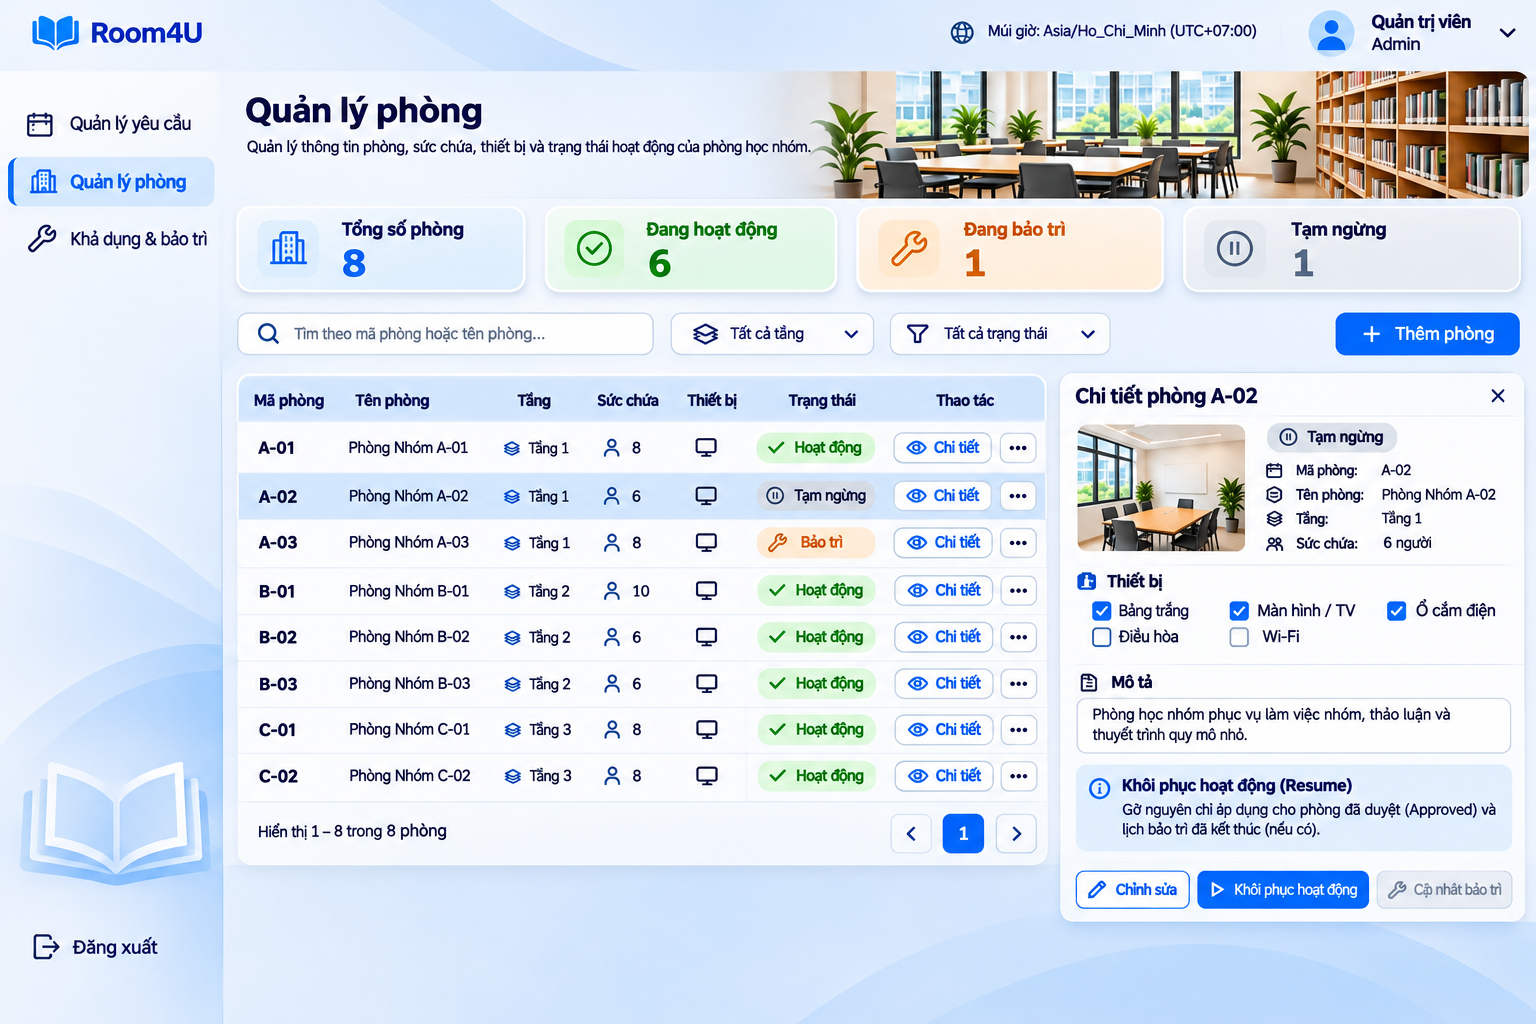
\includegraphics[width=\textwidth,height=0.72\textheight,keepaspectratio]{images/figures/image14.png}
\emph{\textbf{Figure 7.2.7.} S07 -- Room Management.}
\end{center}


\subsubsection{7.2.8. S08 -- Room Availability and
Maintenance}\label{s08-room-availability-and-maintenance}

\textbf{Description:} This screen allows administrators to inspect room
usage and manage maintenance schedules. The interface separates the
room-usage calendar from the maintenance schedule so that Approved
bookings and maintenance records can be reviewed without confusing their
meanings.

\textbf{Room Usage History:} Administrators can inspect room schedules
in the available calendar views and identify Approved bookings,
maintenance periods, and available time slots. The schedule is organized
by room and date to support availability checks.

Maintenance Schedule: Administrators can view existing maintenance
records, create a maintenance schedule, inspect its details, and remove
its effect when eligible. A maintenance record identifies the affected
room, start and end time, reason, and status. The maintenance reason is
required and must contain 1--250 characters after leading and trailing
whitespace are trimmed. The maintenance list provides view and remove
actions; an edit action is not included in the current UC-13 flow.

Maintenance Rules and Removal Flow: To create a maintenance schedule,
the administrator specifies the room, start time, end time, and reason.
The reason is mandatory and must contain 1--250 characters after
trimming leading and trailing whitespace. The end time must be later
than the start time. The system rejects creation if the requested period
overlaps an Approved booking or an active maintenance period.
Maintenance schedules are not subject to booking-specific restrictions:
the 08:00--20:00 operating window, booking-duration options, and
same-calendar-day requirement do not apply. Creating maintenance does
not automatically cancel or modify an Approved booking. To remove a
schedule's effect, the administrator selects a block
that is Active and has not started, reviews the information, and
confirms the action. On success, the system removes the
block's effect on availability, updates the room
schedule, and retains the maintenance record for reference. If the block
has already started or no longer meets the eligibility conditions, the
system displays an error and makes no change to the record.

When maintenance creation returns HTTP 409 with
error.code = SCHEDULE\_CONFLICT, S08 reads error.conflicts and retains
error.requestId as the response correlation identifier. Following SQ05,
if Approved bookings overlap, the API returns those conflicts first, each
with bookingRequestId, startAt and endAt. S08 displays the list and lets
the Administrator open each booking in S06. The Administrator may cancel
a booking only when UC-10 permits it; if it has started or is otherwise
ineligible, S08 instructs the Administrator to choose another time
window. The Administrator returns to S08 and retries after handling any
eligible booking separately. If there is no Approved-booking conflict
but an active maintenance block overlaps, S08 displays its
maintenanceBlockId and interval and instructs the Administrator to
choose another time window. No booking is cancelled automatically.

\textbf{Control Specifications}

\small
\setlength{\tabcolsep}{3pt}
\renewcommand{\arraystretch}{1.15}
\begin{longtable}[]{@{}
  >{\raggedright\arraybackslash}p{0.15557200000000002\textwidth}
  >{\raggedright\arraybackslash}p{0.14885600000000002\textwidth}
  >{\raggedright\arraybackslash}p{0.33147600000000005\textwidth}
  >{\raggedright\arraybackslash}p{0.284096\textwidth}@{}}
\hline
\begin{minipage}[b]{\linewidth}\raggedright
\textbf{Control}
\end{minipage} & \begin{minipage}[b]{\linewidth}\raggedright
\textbf{Type}
\end{minipage} & \begin{minipage}[b]{\linewidth}\raggedright
\textbf{Description and Validation}
\end{minipage} & \begin{minipage}[b]{\linewidth}\raggedright
\textbf{Event Handling}
\end{minipage} \\
\hline
\endhead
\hline
\endlastfoot
\textbf{Room usage calendar} & Calendar & Displays room schedules by
room and date; distinguishes Approved bookings, maintenance, and
available periods. & Changing room/date/view refreshes schedule
information. \\
\textbf{Maintenance interval} & Start/end date and time & End time must
be later than start time; interval is checked against Approved bookings
and active maintenance. Booking-only restrictions (08:00--20:00, booking
duration, and same-day requirement) do not apply. & Invalid interval
displays validation; conflict rejects creation. \\
\textbf{Maintenance reason} & Text area & Required text area; 1--250
characters after leading and trailing whitespace are trimmed. & A valid
reason is stored with the maintenance record; invalid or blank input is
rejected. \\
\textbf{Create maintenance} & Button + confirmation & Creates a record
only when no prohibited overlap exists. & On 409 SCHEDULE\_CONFLICT,
shows error.conflicts. Approved-booking conflicts include booking ID
and interval and link to S06; cancellation is offered only when UC-10
allows it. If a booking has started or an active maintenance block is
the conflict, instructs the Administrator to choose another time.
Successful creation updates the schedule and maintenance list. \\
\textbf{Maintenance list} & List / table & Shows affected room,
start/end time, reason, and status; supports view and eligible removal.
& Selecting a record opens its details. \\
\textbf{Remove maintenance} & Button + confirmation & Only an Active
block that has not started can be removed. & Successful removal
deactivates the block's effect but retains the record;
unsuccessful removal leaves it unchanged. \\
\end{longtable}
\normalsize

\begin{center}
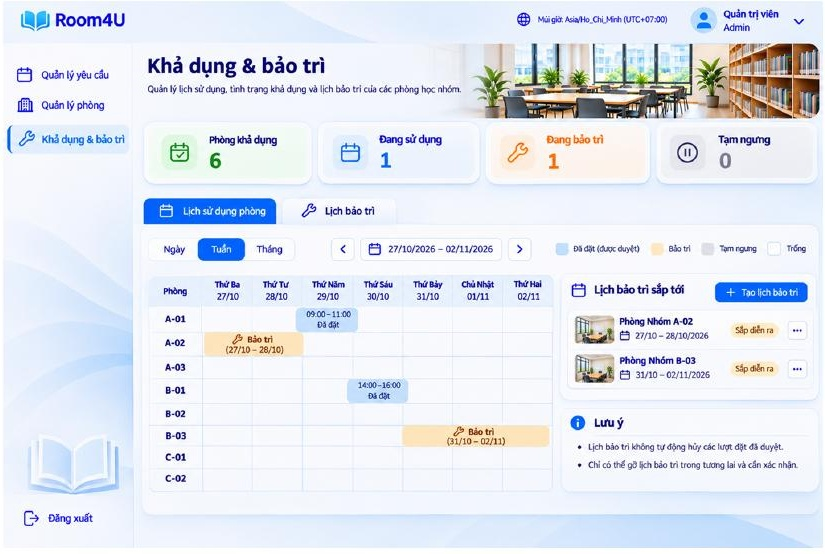
\includegraphics[width=\textwidth,height=0.72\textheight,keepaspectratio]{images/figures/image15.jpg}
\emph{\textbf{Figure 7.2.8.1.} S08.1 -- Room Usage History.}
\end{center}


\begin{center}
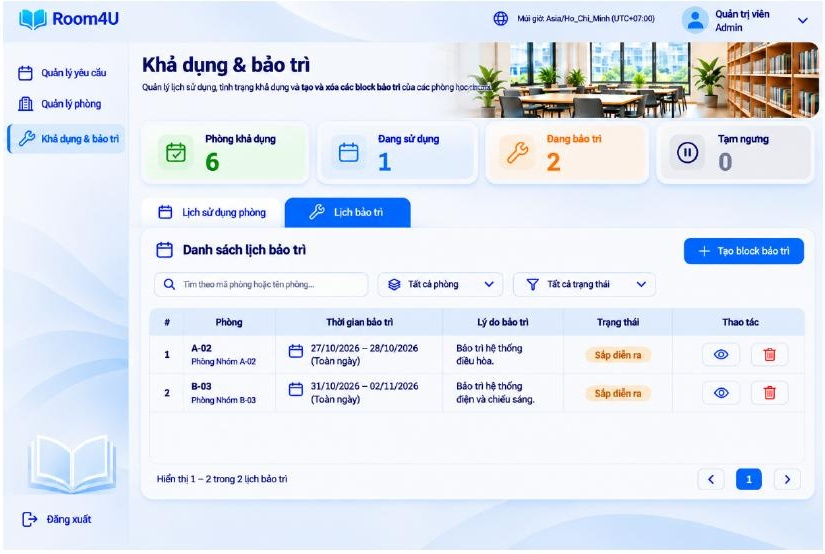
\includegraphics[width=\textwidth,height=0.72\textheight,keepaspectratio]{images/figures/image16.jpg}
\emph{\textbf{Figure 7.2.8.2.} S08.2 -- Maintenance Schedule.}
\end{center}


\subsubsection{7.2.9. UI-to-API Data Mapping}\label{ui-to-api-data-mapping}

The following mapping defines how the affected UI controls correspond to
API/database fields. Field names follow the API contract; purpose and
equipment codes follow the catalogues in ADR-005. Vietnamese labels are
presentation values and do not replace the stored codes.

\small
\setlength{\tabcolsep}{3pt}
\renewcommand{\arraystretch}{1.15}
\begin{longtable}[]{@{}
  >{\raggedright\arraybackslash}p{0.23\textwidth}
  >{\raggedright\arraybackslash}p{0.23\textwidth}
  >{\raggedright\arraybackslash}p{0.23\textwidth}
  >{\raggedright\arraybackslash}p{0.23\textwidth}@{}}
\hline
\begin{minipage}[b]{\linewidth}\raggedright
\textbf{Screen}
\end{minipage} & \begin{minipage}[b]{\linewidth}\raggedright
\textbf{UI control}
\end{minipage} & \begin{minipage}[b]{\linewidth}\raggedright
\textbf{API/database field}
\end{minipage} & \begin{minipage}[b]{\linewidth}\raggedright
\textbf{Data handling}
\end{minipage} \\
\hline
\endhead
\hline
\endlastfoot
S02 & Equipment filters & equipmentCodes & Optional array of equipment
codes (catalogue in ADR-005). Multiple selections use AND logic; an
empty selection applies no equipment filter. \\
S03 & Purpose of use & purpose & Required string purpose code from ADR-005;
submit the code, display its Vietnamese label, and store it in
booking\_requests.purpose. \\
S03 & Optional note & note & Optional string, maximum 250 characters; trim input and normalize blank to NULL. \\
S03 & Submission retry & submissionKey & Required UUID key for one
logical submission; reuse it only when retrying the same unchanged
submission after timeout or uncertain response. \\
S04 & Purpose display & purpose & Read the code from the purpose field
returned by the API (stored in booking\_requests.purpose) and resolve it
to the corresponding Vietnamese display label. \\
S04 & Mô tả chi tiết yêu cầu & note & Display the note value; this is
not a separate field. \\
S07 & Equipment checkboxes & equipmentCodes & Array of codes from ADR-005; required on create, optional on update (omitted means preserve), and an empty array means none selected. Edit Room restores values from API equipmentCodes. \\
S07 & Room list and summary & items, total, summary, asOf,
displayStatus & GET /admin/rooms returns the filtered page and total plus
an all-room summary. One server asOf classifies the list and summary;
suspended takes precedence over active maintenance, then active. \\
S07 & Search and filters & q, floor, status, page, pageSize & Optional
query and pagination inputs to GET /admin/rooms; q matches room code/name
case-insensitively. Filter before pagination and sort by code then ID. \\
S07 & Optional room image & photoRef & Create: blank, omitted or null uses the
default. Update: omission preserves, null clears, and a valid existing
image reference selects. The remove-image action sends null. \\
\end{longtable}
\normalsize

\subsection{Responsive Layout and
Accessibility}\label{responsive-layout-and-accessibility}

\subsubsection{7.3.1. Responsive Layout}\label{responsive-layout}

Room4U uses a desktop-first layout while adapting its interface to
smaller mobile screens. The same business rules and available operations
are retained; only the presentation and arrangement of controls change.

\small
\setlength{\tabcolsep}{3pt}
\renewcommand{\arraystretch}{1.15}
\begin{longtable}[]{@{}
  >{\raggedright\arraybackslash}p{0.169096\textwidth}
  >{\raggedright\arraybackslash}p{0.372048\textwidth}
  >{\raggedright\arraybackslash}p{0.378856\textwidth}@{}}
\hline
\begin{minipage}[b]{\linewidth}\raggedright
\textbf{Interface Element}
\end{minipage} & \begin{minipage}[b]{\linewidth}\raggedright
\textbf{Desktop Layout}
\end{minipage} & \begin{minipage}[b]{\linewidth}\raggedright
\textbf{Mobile Layout}
\end{minipage} \\
\hline
\endhead
\hline
\endlastfoot
\textbf{Header} & Room4U branding, account information, and navigation
controls. & Compact header to preserve screen space. \\
\textbf{Sidebar} & Vertical navigation items. & Compact or collapsible
navigation. \\
\textbf{Room cards} & Multiple room cards in a grid. & Cards stacked
vertically. \\
\textbf{Booking form} & Structured form layout with grouped fields. &
Fields stacked vertically without changing duration-based booking
input. \\
\textbf{Request tables} & Tabular request information. & Compact cards
or responsive list to avoid page-level horizontal scrolling. \\
\textbf{Availability calendar} & Schedule with space for time-slot
information. & Simplified or horizontally manageable schedule. \\
\textbf{Dialogs} & Confirmation and result dialogs over the current
screen. & Dialog width adapts to viewport while keeping actions
readable. \\
\end{longtable}
\normalsize

Proposed verification viewport sizes are Desktop 1366 × 768 pixels and
Mobile 390 × 844 pixels. The layout should avoid fixed-width page
containers that cause horizontal scrolling. The PA2 mockups provide the
desktop visual baseline; the PA3 mobile layout is a responsive proposal
and must be verified during implementation.

\subsubsection{7.3.2. Accessibility
Considerations}\label{accessibility-considerations}

\small
\setlength{\tabcolsep}{3pt}
\renewcommand{\arraystretch}{1.15}
\begin{longtable}[]{@{}
  >{\raggedright\arraybackslash}p{0.16238\textwidth}
  >{\raggedright\arraybackslash}p{0.39909600000000006\textwidth}
  >{\raggedright\arraybackslash}p{0.358524\textwidth}@{}}
\hline
\begin{minipage}[b]{\linewidth}\raggedright
\textbf{Checklist Item}
\end{minipage} & \begin{minipage}[b]{\linewidth}\raggedright
\textbf{Proposed Implementation}
\end{minipage} & \begin{minipage}[b]{\linewidth}\raggedright
\textbf{Verification Required}
\end{minipage} \\
\hline
\endhead
\hline
\endlastfoot
\textbf{Contrast and meaning} & Text contrast ≥4.5:1; status meaning is
conveyed by text labels, not color alone. & Measure actual implemented
colors; do not claim compliance from wireframes. \\
\textbf{Keyboard access} & Native buttons/links, logical tab order,
visible focus, and dialog focus restoration. & Walk through sign-in,
search, submit, cancel, and approve. \\
\textbf{Labels and errors} & Persistent labels; field-error
associations; status region; preserve safe values. & Verify announced
errors, confirmation dismissal, and retry behavior. \\
\textbf{Responsive layout} & Stack cards/forms; avoid fixed-width page;
mobile list cards instead of wide tables. & Test Chrome/Edge at 390×844
and 1366×768; no horizontal page scroll. \\
\textbf{Usability} & Show that Pending is not confirmed; display
room/capacity/time context. & Run the actual PA2 four-evaluator task; do
not invent participant outcomes. \\
\textbf{Localization} & Vietnamese labels and reason/error messages;
visible Asia/Ho\_Chi\_Minh time zone. & Review S01--S08 strings and
date/time conversions. \\
\end{longtable}
\normalsize

\subsubsection{7.3.3. User Feedback and Error
Communication}\label{user-feedback-and-error-communication}

\begin{itemize}
\item
  Display success feedback only after the system confirms that an
  operation has completed.
\item
  Identify missing or invalid input and explain how the user can correct
  it.
\item
  Explain scheduling conflicts and show relevant current information
  without modifying conflicting records automatically.
\item
  Use confirmation dialogs for important operations, including booking
  submission, cancellation, approval, rejection, room
  suspension/resumption, and maintenance removal where applicable.
\item
  Preserve valid input after known validation or conflict failures so
  users can correct the request.
\item
  Clearly distinguish Pending from Approved; a Pending request is
  awaiting administrator review and is not a confirmed reservation.
\end{itemize}

\subsubsection{7.3.4. Usability and
Localization}\label{usability-and-localization}

The interface should show sufficient context for users to make correct
decisions. Before submitting a booking request, students should be able
to review the selected room, room capacity, usage date, start time,
duration, and calculated end time. Before administrative actions,
administrators should be able to inspect the current request or room
state.

The interface uses Vietnamese labels and messages to maintain
consistency with the target users and NFR-12. Dates and times use the
Asia/Ho\_Chi\_Minh time zone where applicable.

The usability evaluation should verify that users can complete the
following main tasks:

\begin{enumerate}
\def\labelenumi{\arabic{enumi}.}
\item
  Sign in using a provided account.
\item
  Search for a suitable meeting room.
\item
  Inspect room availability.
\item
  Submit a booking request.
\item
  Review request status and history.
\item
  Cancel an eligible booking request.
\item
  Process a booking request as an administrator.
\item
  Manage room information and maintenance schedules.
\end{enumerate}

The evaluation must follow the actual PA2 evaluation procedure and
record real observations. No participant outcomes or usability results
are assumed in this design document.


\section{Traceability Update}
This matrix replaces PA2 planned design topics with concrete identifiers in the current proposed PA3 design. The identifiers refer to artifacts present in this draft, not an accepted implementation. PA4 and PA5 verification remains planned. PA2 Section 6 supplies the requirement definitions and original PA1/D01--D08 source mapping; this design does not silently alter that source.

Coverage spans 27 functional requirements, 12 non-functional requirements, and 16 business rules (55 unique entries). A screen represents a user-facing realization rather than proof of backend enforcement. M01 protects authenticated operations. Commands that modify an existing room or its schedule acquire the room guard through C08.

\subsection{Functional Requirements}
\begingroup
\small
\setstretch{1.0}
\setlength{\tabcolsep}{2pt}
\renewcommand{\arraystretch}{1.1}
\begin{longtable}{|>{\raggedright\arraybackslash}p{0.07\textwidth}|>{\raggedright\arraybackslash}p{0.25\textwidth}|>{\raggedright\arraybackslash}p{0.09\textwidth}|>{\raggedright\arraybackslash}p{0.40\textwidth}|>{\raggedright\arraybackslash}p{0.12\textwidth}|}
\hline
\shortstack{\textbf{Req.}\\\textbf{ID}} & \textbf{Component, class, or sequence} & \textbf{Screen} & \textbf{Data or design element} & \textbf{Planned verification} \\
\hline
\endfirsthead
\hline
\shortstack{\textbf{Req.}\\\textbf{ID}} & \textbf{Component, class, or sequence} & \textbf{Screen} & \textbf{Data or design element} & \textbf{Planned verification} \\
\hline
\endhead
\hline
\endfoot
\hline
\endlastfoot
FR-01 & M01; C07; C12 & S01 & ADR-003; \texttt{users.firebase\_uid} & AC-01 \\ \hline
FR-02 & M01; C07 & S01--S08 & 401 guard; no-store private responses & AC-02 \\ \hline
FR-03 & M01; C07; M02 & S01--S08 & Server role map; route role table & AC-02 \\ \hline
FR-04 & M03; C14; C04 & S04 & \texttt{booking\_requests.owner\_id} equals the authenticated application user ID & AC-02; AC-08 \\ \hline
FR-05 & CT1 session adapter & S02--S08 & Clear SDK session and private DTOs & AC-03 \\ \hline
FR-06 & M03; C14 & S02 & \texttt{rooms} and \texttt{room\_equipment} safe DTO (\texttt{equipmentCodes} and display descriptions); placeholder photo; ADR-005 & AC-04 \\ \hline
FR-07 & M03; C14 & S02 & \texttt{rooms} capacity filter; local-date window & AC-04 \\ \hline
FR-08 & M03; C14; DB01 & S02 & \texttt{room\_occupancy}; Pending absent & AC-05 \\ \hline
FR-09 & M03; C14 & S02 & State label; identity-free calendar DTO & AC-05; AC-02 \\ \hline
FR-10 & M06; C03; SQ01 & S03 & ADR-004; ADR-005; room lock, eligibility policy, categorized purpose, and note ($\leq 250$ characters) & AC-06; AC-07 \\ \hline
FR-11 & M04; C04; SQ01 & S03; S04 & \texttt{booking\_requests} with categorized purpose and note ($\leq 250$ characters), plus creation event; no occupancy; ADR-005 & AC-06 \\ \hline
FR-12 & M03; C14 & S04 & Role-scoped detail (purpose, note, permitted requester information) and ordered \texttt{booking\_events}; ADR-005 & AC-08 \\ \hline
FR-13 & M04; C01; SQ03 & S04 & Cancellation ChangeSet and release & AC-09 \\ \hline
FR-14 & M03; C14 & S05; S06 & Default Pending and Approved filter & AC-10; queue/filter inspection \\ \hline
FR-15 & M04; C04; SQ02 & S06 & C03 policy; atomic approval ChangeSet & AC-10; AC-11 \\ \hline
FR-16 & M07; C08; SQ02; SQ05 & S06; S07; S08 & ADR-002; shared exclusion and room guard & AC-11; AC-12; NFR-03 method \\ \hline
FR-17 & M04; C01; C04 & S06; S04 & Pending $\rightarrow$ Rejected; reason event & AC-13 \\ \hline
FR-18 & M04; C01; C04 & S06; S04 & Administrator cancellation with reason and release & AC-14 \\ \hline
FR-19 & M04; C08 & S04; S06 & Append-only \texttt{booking\_events} in command transaction & AC-06; AC-08; AC-10; AC-13--14 \\ \hline
FR-20 & M05; C02; C05; C09; C14 & S07 & Atomic room/equipment save; GET /admin/rooms filtered list, stable order, displayStatus and unfiltered summary & AC-15 \\ \hline
FR-21 & M05; C05; SQ04 & S07 & Room guard; future Approved maximum; atomic \texttt{room\_equipment} update in one transaction; ADR-005 & AC-15; capacity/approval race design \\ \hline
FR-22 & M05; C05; U06 & S07 & State command under room guard & AC-16 \\ \hline
FR-23 & M05; C05; U06 & S07 & Resume without releasing occupancy & AC-16 \\ \hline
FR-24 & M05; C06; SQ05 & S08 & \texttt{maintenance\_blocks} and occupancy & AC-17 \\ \hline
FR-25 & M05; C06; SQ05 & S08; S06 & SCHEDULE\_CONFLICT DTO; Approved-booking conflicts first, explicit UC-10 eligibility handoff; maintenance-block conflict otherwise & AC-12; AC-17 \\ \hline
FR-26 & M05; C06; C10; U06 & S08 & Retained removed block; delete projection & AC-18 \\ \hline
FR-27 & M03; M05; C14 & S02; S07; S08 & Reread committed data after mutation; S07 refreshes list and summary & AC-15--18 \\ \hline
\end{longtable}
\endgroup

\subsection{Non-Functional Requirements}
\begingroup
\small
\setstretch{1.0}
\setlength{\tabcolsep}{2pt}
\renewcommand{\arraystretch}{1.1}
\begin{longtable}{|>{\raggedright\arraybackslash}p{0.07\textwidth}|>{\raggedright\arraybackslash}p{0.22\textwidth}|>{\raggedright\arraybackslash}p{0.12\textwidth}|>{\raggedright\arraybackslash}p{0.36\textwidth}|>{\raggedright\arraybackslash}p{0.16\textwidth}|}
\hline
\textbf{Req.} & \textbf{Design realization} & \textbf{Screen} & \textbf{Mechanism} & \textbf{Planned verification} \\
\hline
\endfirsthead
\hline
\textbf{Req.} & \textbf{Design realization} & \textbf{Screen} & \textbf{Mechanism} & \textbf{Planned verification} \\
\hline
\endhead
\hline
\endfoot
\hline
\endlastfoot
NFR-01 & M03; C14; query indexes & S02; S04 & Paged reads and bounded DTOs; reference workload and dataset as defined in PA2 Section 6.2; measurement planned for PA4 & PA2 Section 6.2 NFR-01 load method \\ \hline
NFR-02 & M01; C07; M02 & All private screens & 401/403 role and owner enforcement & PA2 Section 6.2 NFR-02 negative matrix \\ \hline
NFR-03 & M07; C08; ADR-002 & S06; S07; S08 & Room guard, exclusion, and rollback & PA2 Section 6.2 NFR-03 race trials \\ \hline
NFR-04 & CT1 semantic controls & S01--S08 & Labels, focus, error association, and contrast & PA2 Section 6.2 NFR-04 walkthrough \\ \hline
NFR-05 & CT1 request journey & S02--S04 & Visible Pending explanation and short form & PA2 Section 6.2 NFR-05 real evaluator task \\ \hline
NFR-06 & M01; A04 deployment & All screens & HTTPS, secrets outside repository, no token logging & PA2 Section 6.2 NFR-06 inspection \\ \hline
NFR-07 & CT1 responsive layout & S01--S08 & 390/1366 widths; no unavailable control & PA2 Section 6.2 NFR-07 browser smoke \\ \hline
NFR-08 & A04 backup procedure & N/A operational & Restricted backup and timed restore inventory & PA2 Section 6.2 NFR-08 restore drill \\ \hline
NFR-09 & M07; C08; ADR-002 & S03--S08 & Same-client transaction; no partial source/event & PA2 Section 6.2 NFR-09 failure injection \\ \hline
NFR-10 & \texttt{booking\_events}; C08 & S04; S06 & Immutable booking events and stable ordering & PA2 Section 6.2 NFR-10 event inspection \\ \hline
NFR-11 & M02; C03; CT1 errors & S03; S06--S08 & FieldErrors, preserved non-sensitive values & PA2 Section 6.2 NFR-11 boundary cases \\ \hline
NFR-12 & CT1 i18n; ADR-004 & S01--S08 & Vietnamese labels and visible local zone & PA2 Section 6.2 NFR-12 inventory \\ \hline
\end{longtable}
\endgroup

\subsection{Business Rules}
\begingroup
\small
\setstretch{1.0}
\setlength{\tabcolsep}{2pt}
\renewcommand{\arraystretch}{1.1}
\begin{longtable}{|>{\raggedright\arraybackslash}p{0.07\textwidth}|>{\raggedright\arraybackslash}p{0.20\textwidth}|>{\raggedright\arraybackslash}p{0.12\textwidth}|>{\raggedright\arraybackslash}p{0.36\textwidth}|>{\raggedright\arraybackslash}p{0.18\textwidth}|}
\hline
\textbf{Rule} & \textbf{Design realization} & \textbf{Screen} & \textbf{Mechanism} & \textbf{Planned verification} \\
\hline
\endfirsthead
\hline
\textbf{Rule} & \textbf{Design realization} & \textbf{Screen} & \textbf{Mechanism} & \textbf{Planned verification} \\
\hline
\endhead
\hline
\endfoot
\hline
\endlastfoot
BR-01 & M01; C07; C04 & S01; S03 & Seeded roles; one request owner and room & AC-01; AC-06 \\ \hline
BR-02 & M06; C03 & S03; S06 & Local opening-hour check & AC-07 \\ \hline
BR-03 & M06; C03; ADR-004 & S03; S06 & Start increment and permitted duration list & AC-07 plus discrete-duration cases \\ \hline
BR-04 & M06; C03; C08 & S03; S06 & Decision clock after room lock & AC-07; AC-11 \\ \hline
BR-05 & C02; C03; C05; SQ04 & S02; S03; S06; S07 & Current capacity; future booking safety & AC-04; AC-07; AC-15 \\ \hline
BR-06 & C03; \texttt{room\_occupancy} & S02; S03; S06; S08 & Half-open \texttt{tstzrange} [start, end) & AC-07; AC-11; AC-17 \\ \hline
BR-07 & C04; DB01 & S02; S03; S06 & Only Approved bookings and active maintenance occupy & AC-05; AC-06; AC-11 \\ \hline
BR-08 & C08; ADR-002; SQ02 & S06; S08 & Atomic current-data approval & AC-11; AC-12 \\ \hline
BR-09 & C01; U05 & S03; S04; S06 & Four-state transition guards & AC-06; AC-09--14 \\ \hline
BR-10 & C01; C04; SQ03 & S04; S06 & Before-start cancellation; late Pending rejection & AC-09; AC-13; AC-14 \\ \hline
BR-11 & C05; U06 & S03; S06; S07 & Suspension gate; no occupancy removed & AC-16 \\ \hline
BR-12 & M02 command DTOs; C01 & S03; S04; S06 & No direct room/time edit or admin impersonation & AC-14; API route inspection \\ \hline
BR-13 & C01; C06; C10 & S06; S08 & Trim reason; maintenance time rules separate & AC-13; AC-14; AC-17 \\ \hline
BR-14 & C02; C05; SQ04 & S07 & Unique normalized room code and safe edit & AC-15 \\ \hline
BR-15 & C06; SQ05; DB01 & S06; S08 & Explicit cancellation; retained removed block & AC-12; AC-17; AC-18 \\ \hline
BR-16 & C14; \texttt{booking\_events} & S02; S04; S05; S06 & Owner/admin detail; safe shared DTO & AC-02; AC-05; AC-08 \\ \hline
\end{longtable}
\endgroup

\textbf{Scope and verification note:} History retention scopes remain strictly separated. NFR-10 maps exclusively to immutable, append-only booking lifecycle events (\texttt{booking\_events}), whereas maintenance record retention is traced independently through FR-26, BR-15, and AC-18. Removed records remain soft-retained in \texttt{maintenance\_blocks}, while only the active \texttt{room\_occupancy} projection is deleted; this does not silently expand NFR-10. For PA4 test design, capacity-edit race conditions and all discrete duration boundaries (30, 60, 90, and 120 minutes) must be instantiated as concrete test cases. No test IDs or passing results are claimed in this design baseline.

\clearpage

\section{Changes to the Requirements Since the Previous Baseline}
This section records UI/input-rule refinements and technical design realizations agreed upon since formal approval of the Room4U Software Requirements Specification (SRS), Version 1.0 (PA2 baseline).

\textbf{Distinction between requirement scope and design realization:} The core functional and business policies established in the PA2 SRS v1.0 baseline remain intact: duration-based booking input; the four request lifecycle states (Pending, Approved, Rejected, and Cancelled); non-blocking Pending requests, with occupancy reserved only upon approval; and soft-retained \texttt{maintenance\_blocks} records after removal. Adding database columns or tables, such as user profile attributes or \texttt{room\_equipment}, to support fields already represented in UI screens, or adopting ADR-001 through ADR-005, represents a concrete technical realization or input-contract refinement rather than a new functional requirement or a silent rewrite of existing FR/BR definitions.

\begingroup
\footnotesize
\setstretch{1.0}
\setlength{\tabcolsep}{2pt}
\renewcommand{\arraystretch}{1.1}
\begin{longtable}{|>{\raggedright\arraybackslash}p{0.07\textwidth}|>{\raggedright\arraybackslash}p{0.14\textwidth}|>{\raggedright\arraybackslash}p{0.29\textwidth}|>{\raggedright\arraybackslash}p{0.24\textwidth}|>{\raggedright\arraybackslash}p{0.20\textwidth}|}
\hline
\textbf{Item} & \textbf{Category} & \textbf{Nature of refinement / decision} & \textbf{Rationale} & \textbf{Affected items} \\
\hline
\endfirsthead
\hline
\textbf{Item} & \textbf{Category} & \textbf{Nature of refinement / decision} & \textbf{Rationale} & \textbf{Affected items} \\
\hline
\endhead
\hline
\endfoot
\hline
\endlastfoot
DR-01 & Technical design realization & Room-level lock guard (C08) paired with a shared \texttt{room\_occupancy} projection (\texttt{tstzrange} exclusion). & Makes existing concurrency, double-booking prevention, and safe capacity-edit requirements deterministic and executable at the database level. & ADR-002; FR-15--16, FR-21, FR-24--26; NFR-03, NFR-09; BR-06, BR-08. No new user operation. \\ \hline
DR-02 & Technical design realization & Idempotency submission key and explicit replay response handling. & Guarantees one booking request and one initial \texttt{booking\_events} record when a client retries a logical submission after network interruption. & FR-11, FR-19; NFR-09; SQ01. Aligns API and PA4 retry-test expectations. \\ \hline
DR-03 & Technical design realization & Concrete REST API DTO contracts, structured error codes (\texttt{FieldErrors}), and relational storage schemas, including the S07 administrative room-list/summary contract and S08 maintenance-conflict DTO. & Establishes unambiguous contracts across the web interface (CT1), domain policies, and PostgreSQL persistence without changing PA2 business rules. & Sections 4--8; FR-20, FR-24--27; S07, S08; NFR-11. Design detail, not a new requirement. \\ \hline
DR-04 & UI/input-rule refinement (ADR-005) & Standardizes purpose selection as a fixed category-code list, stored as normalized codes in \texttt{booking\_requests} and mapped to localized Vietnamese UI labels; the note remains optional and is capped at 250 characters. & Eliminates free-text ambiguity for booking purposes while keeping validation uniform across frontend forms and backend command DTOs. & ADR-005; FR-10--12; S03, S04, S06; \texttt{booking\_requests} schema. Preserves existing eligibility rules. \\ \hline
DR-05 & Technical design realization (ADR-005) & Extends the \texttt{users} table with profile fields to store and display requester identity details in authorized views. & Supports displaying permitted user information already expected by the UI without creating a separate user-management feature. & ADR-005; FR-01, FR-04, FR-12; BR-16; S04, S06; \texttt{users} schema. \\ \hline
DR-06 & UI/input-rule refinement (ADR-005) & Removes the standalone Related course field from screen S04 (Request Detail) and removes room area/zone metadata while retaining floor information. & Streamlines request details and room metadata to align the UI with the agreed Room4U data model and avoid redundant input fields. & ADR-005; FR-06, FR-12; S02, S04, S07; rooms and \texttt{booking\_requests} UI/DTO contracts. \\ \hline
DR-07 & UI/input-rule and data refinement (ADR-005) & Standardizes room amenities through the normalized \texttt{room\_equipment} table, with multi-select checkboxes on room management/search screens and multi-amenity filtering using strict AND semantics. & Replaces unstructured facility text with consistent equipment codes (\texttt{equipmentCodes}) and human-readable labels, ensuring search results match all selected amenities. & ADR-005; FR-06--07, FR-20--21; S02, S07; \texttt{room\_equipment} schema (AC-04, AC-15). \\ \hline
CR Status & Baseline governance & Active design refinements DR-01--DR-07 are recorded; no formal PA2 FR/BR rewrite has been approved. The S07 list/summary and S08 conflict response are PA3 API/UI design details supporting existing screens and use cases; they do not add or change requirements. Other post-PA2 updates remain ADR-005 UI/input-contract refinements and ADR-001--ADR-005 technical realizations. & Avoids conflating UI field cleanups, API contract detail and schema realizations with formal requirement changes while keeping an explicit record of agreed adjustments. & Any future change to core PA2 rules, such as switching booking input from duration to explicit end time, must follow formal change control across PA2 SRS v1.0, UC-04/UC-14, S03, AC scenarios, and PA3. \\ \hline
\end{longtable}
\endgroup

\clearpage

\section{AI Usage Log}

This section is required in every PA under the course GenAI policy. List each significant use of AI tools. Write ``No AI tools were used'' if none. Undisclosed AI use is treated as an academic integrity violation.

\begingroup
\small
\setstretch{1.0}
\setlength{\tabcolsep}{3pt}
\renewcommand{\arraystretch}{1.1}
\begin{longtable}{|>{\raggedright\arraybackslash}p{0.05\textwidth}|>{\raggedright\arraybackslash}p{0.22\textwidth}|>{\raggedright\arraybackslash}p{0.16\textwidth}|>{\raggedright\arraybackslash}p{0.20\textwidth}|>{\raggedright\arraybackslash}p{0.28\textwidth}|}
\hline
\textbf{\#} & \textbf{Member} & \textbf{Tool} & \textbf{Task / purpose} & \textbf{How the output was verified and changed} \\ \hline
\endfirsthead
\hline
\textbf{\#} & \textbf{Member} & \textbf{Tool} & \textbf{Task / purpose} & \textbf{How the output was verified and changed} \\ \hline
\endhead
\hline
\endfoot
\hline
\endlastfoot
1 & Nguyễn Kim Ngân & ChatGPT & Assisted in preparing Section 7 -- UI/UX Design, including organizing design documentation, describing UI screens, and improving the clarity and consistency of the content. & Reviewed the generated content against the project requirements, existing UI/UX designs, and related documentation. Corrected wording, updated details to match the actual Room4U design, and retained only relevant content. \\ \hline
2 & Nguyễn Kim Ngân & ChatGPT & Assisted in assembling and formatting the PA3 report, including converting and revising documentation into LaTeX. & Checked the generated LaTeX against the report template, verified section structure and image paths, and compiled the document to identify and correct formatting or compilation errors. \\ \hline
3 & Nguyễn Thành Long & Gemini & Assisted in drafting and reviewing project requirements and business rules, checking grammar, and preparing the change form for the project since PA2. & Reviewed the generated content and LaTeX for accuracy and consistency, cross-checked it with the team, and revised it based on team feedback. \\ \hline
4 & Trần Thiên Phúc & ChatGPT & Reviewed the PA3 PDF layout in Sections 3, 4, 6, and 7. ChatGPT flagged HTTP/JSON and SQL blocks split across pages, API routes displaying \texttt{allowbreak}, a cramped table, and an outdated ERD missing \texttt{room\_equipment}; it also drafted a prompt for LaTeX revisions. & A follow-up ChatGPT review compared the revised PDF with the earlier version. It confirmed that the room-search route displayed correctly, the HTTP/JSON and SQL examples were formatted as code blocks, and the updated ERD contained all seven tables, including room_equipment. \\ \hline
5 & Trần Thiên Phúc & ChatGPT & Reviewed group PR updates against earlier feedback, checked consistency among descriptions, diagrams, and traceability tables, and drafted PR feedback. Examples: Lại Minh Thông's Section 5 and Nguyễn Thành Long's Sections 1, 8, and 9. & The AI-assisted review checked the revised documents against earlier feedback. For Section 5, it cross-checked the diagrams with the class specifications and written explanations. The resulting comments were provided as drafts for my review.\\ \hline
6 & Lại Minh Thông & Claude & Used Claude to turn my design descriptions into code for generating the Section 5 diagrams, complete details in the class specifications and diagrams, apply changes requested during the team review, and clarify the wording. & Checked that the diagrams, class specifications, and explanations were consistent with one another and with the use cases. Rewrote or removed inaccurate or unclear output; the team reviewer also checked the AI-assisted content before it was retained. \\ \hline
7 & Lại Minh Thông & ChatGPT & Used ChatGPT to help write and format the LaTeX for Section 5, including integrating the diagrams, class specifications, and explanatory text into the report. & Compiled and reviewed the rendered document, checked the figure paths and table formatting, and corrected the LaTeX output to match the approved Section 5 content. \\ \hline
\end{longtable}
\endgroup


\clearpage

%% Items that require confirmation from the project team.

\section*{Items Pending Team Confirmation}
\addcontentsline{toc}{section}{Items Pending Team Confirmation}

\begin{itemize}
  \item \textbf{[Phuc and Ngân to confirm]} the S07 API contract for reading the room list, applying floor and status filters, and returning total and per-status room counts.
  \item \textbf{[Phuc to confirm]} whether \texttt{docs/design/data/schema.sql} is included in the editable source package intended for submission.
  \item \textbf{[Phuc to confirm]} the exact source titles and locations for the team's PA1 and accepted PA2 documents so the project references can match the original documents.
\end{itemize}

\clearpage

% References cited in the PA3 design.

\section*{References}
\addcontentsline{toc}{section}{References}

\begin{description}[leftmargin=1.1cm,style=nextline]
  \item [P1] Room4U Project Assignment 1 (PA1), submitted by team T03.
  \item [P2] Room4U Software Requirements Specification (SRS), Version 1.0 (PA2).
  \item [R1] PostgreSQL Documentation, \emph{Explicit Locking}. \url{https://www.postgresql.org/docs/current/explicit-locking.html}
  \item [R2] PostgreSQL Documentation, \emph{Range Types}. \url{https://www.postgresql.org/docs/current/rangetypes.html}
  \item [R5] PostgreSQL Documentation, \emph{Transaction Isolation}. \url{https://www.postgresql.org/docs/current/transaction-iso.html}
\end{description}

% ==================================================
% END OF DOCUMENT
% ==================================================

\end{document}
